%_____________________________________________________________________________
%=============================================================================
% main.tex v8 (31-05-2015) \ldots dibuat oleh Lionov - Informatika FTIS UNPAR
% 
% Ini adalah file utama (main.tex), berisi perintah-perintah yang khusus 
% dibuat untuk template ini
%
% 			JANGAN MENGUBAH APAPUN DI DALAM FILE INI,
%			KECUALI ANDA TAHU APA YANG ANDA LAKUKAN !!!
%
% Jika ada tambahan perintah, dapat anda tuliskan di tempat yang telah disediakan 
% di baris 310 pada file ini
% Jika daftar tabel tidak digunakan, anda harus menghapus (beri komentar) secara
% manual di baris 485
%
% Bug, kritik, saran: silahkan kirimkan via email ke lionov@unpar.ac.id
%
% Perubahan pada versi 8 (31-05-2015):
%	- penambahan default data untuk beberapa keterangan dan digunakan sebagai 
%	  template dengan tanda << & >> . Data yang diubah defaultnya adalah: nama skripsi
%	  nama prodi, beserta bahasa inggrisnya.
%   - Keywords dan kata kunci di abstrak ditambahkan noindent + perbaikan lainnya
%   - Perbaikan untuk halaman tidak kosong tanpa nomor halaman romawi
%
% Perubahan pada versi sebelumnya :
%	versi 7 (27-05-2014)
%	- penambahan perintah \raggedbottom untuk menghilangkan area kosong akibat 
%	  penempatan gambar yang tidak sempurna
%	versi 6 (10-11-2013)
%	- perbaikan pada abstract dengan paragraf lebih dari satu: perbaikan vertical spacing
%	- perbaikan pada tampilan bab dan lampiran: tidak perlu menuliskan apapun untuk 
%	  menampilkan semuanya (di data.tex) atau -1 jika tidak ada lampiran
%	- halaman bernomor genap untuk halaman romawi sudah dimunculkan
%	- Kurikulum 2013 : perubahan nama buku skripsi 
%	versi 5 (21-10-2012)
%	- halaman terakhir setiap bab tidak ada headernya jika kosong
%	versi 4 (06-08-2012)
% 	- penggabungan main.tex, depan.tex dan setup.tex menjadi main.tex
% 	- menambahkan keterangan di lampiran untuk kode program 
% 	- ukuran font dapat diubah langsung di tiap lampiran
% 	versi 3 (09-07-2012): 
%	- Tidak ada di file ini
% 	versi 2 :
% 	- "Daftar Referensi" tidak perlu diubah secara manual (tidak perlu mengubah file bahasai.ldf)
% 	- Bahasa Indonesia dari abstract adalah abstrak (secara otomatis), bukan ringkasan
% 	- Spasi pada buku dokumen final adalah onehalfspacing
%
% to do : - hilangkan secara otomatis daftar tabel/gambar jika tidak digunakan
%         - (IT) aturan penulisan algoritma untuk IT (pakai algo.sty ?)
%=============================================================================

%=============================================================================
% setup.tex v2 (08-07-2012)
% Perubahan pada versi 2:
% - Menambahkan perintah untuk judulINA dan judulENG
% - Menghapus \usepackage{microtype}, yang pada beberapa kasus menjadi masalah
%=============================================================================
% depan.tex v2 (09-07-2012)
% Perubahan pada versi 2:
% - Menambahkan halaman depan dalam bahasa inggris
%=============================================================================

%setup.tex
\documentclass[11pt,a4paper,twoside,openright,notitlepage]{report} 

\usepackage[bahasa]{babel} %bahasa indonesia
\usepackage[T1]{fontenc}  %encoding
% \usepackage{mathptmx}
% \usepackage{venturisold}
% \usepackage{helvet}
% \usepackage{fouriernc} 
\usepackage{abstract} %manipulasi abstract
\usepackage{chappg} % format daftar isi 
\usepackage{color} %warna
\usepackage{etoolbox} %untuk programming if-then
\usepackage{fancyhdr} %format header & footer
\usepackage{float} %penempatan gambar di tempat yg seharusnya
\usepackage[inner=2.5cm,outer=2cm,top=2.5cm,bottom=2.5cm]{geometry} %margin
\usepackage{graphicx} %gambar
\usepackage{listings} %source code
\usepackage{lscape} %landscape untuk source code
\usepackage{multicol} %multiple column
\usepackage{ifthen} % if then
\usepackage[pagewise]{lineno} %line numbering
\usepackage{lipsum} % untuk testing
\usepackage{titlesec} %judul header
\usepackage{tocbibind} %daftar isi, gambar, tabel dll
\usepackage{tocloft} % format daftar isi 
\usepackage{setspace} %line spacing
\usepackage{xstring} %manipulasi string
\usepackage[plainpages=false,pdfpagelabels,unicode]{hyperref} %\autoref, \phantomsection & link 
\usepackage{emptypage}

\let\abstractname\Abstrak

\titleformat{\chapter}[display] {\Large\bfseries\centering}{\MakeUppercase{\chaptertitlename} \thechapter}{15pt}{\Large\MakeUppercase}

\renewcommand{\cftchapfont}{\scshape \bfseries}

\renewcommand{\cfttoctitlefont}{\hfill\Large\bfseries\MakeUppercase}
\renewcommand{\cftaftertoctitle}{\hfill}
\renewcommand{\cftloftitlefont}{\hfill\Large\bfseries\MakeUppercase}
\renewcommand{\cftafterloftitle}{\hfill}
\renewcommand{\cftlottitlefont}{\hfill\Large\bfseries\MakeUppercase}
\renewcommand{\cftafterlottitle}{\hfill}

% Tidak perlu ada kata "Bab", "Gambar" atau "Tabel" di daftar 
% \renewcommand{\cftchappresnum}{{\bf \scshape Bab} } 
% \renewcommand{\cftchapnumwidth}{1.5cm}
% \renewcommand{\cftfigpresnum}{{Gambar\ }} 
% \renewcommand{\cftfignumwidth}{2.5cm}
% \renewcommand{\cfttabpresnum}{{Tabel\ }} 
% \renewcommand{\cfttabnumwidth}{2cm}

\newcommand{\apptoc}{
	% Hapus kata "Lampiran" dari daftar isi
	%\addtocontents{toc}{\protect\renewcommand{\protect\cftchappresnum}{\bf \scshape Lampiran\  }}%
	%\addtocontents{toc}{\protect\renewcommand{\protect\cftchapnumwidth}{2.75cm}}
	\addtocontents{toc}{\protect\renewcommand{\protect\cftchappresnum}{\bf \scshape}}%	

}

\newcommand{\vnama}{Jane Doe}
\newcommand{\vlnama}{John Doe}
\newcommand{\vnpm}{1992700001}
\newcommand{\vprodiINA}{SAINS}
\newcommand{\vprodiENG}{SCIENCE}
\newcommand{\vstaINA}{UJIAN}
\newcommand{\vstaENG}{EXAM}
%\newcommand{\vjudul}{Judul Skripsi/Tugas Akhir}
\newcommand{\vpembu}{Plato}
\newcommand{\vpembs}{Euclid}
\newcommand{\vpengi}{Plato}
\newcommand{\vpengii}{Euclid}
\newcommand{\vtanggal}{1}
\newcommand{\vbulan}{Januari}
\newcommand{\vtahun}{1970}
\newcommand{\vmode}{final}
\newcommand{\vspacing}{double}
\newcommand{\vlineno}{yes}
\newcommand{\vkunciina}{Skripsi, Tugas Akhir}
\newcommand{\vkuncieng}{Undergraduate Thesis, Final Project}
\newcommand{\vkajur}{Jack Doe}
\newcommand{\vkajurmat}{Jack Doe}
\newcommand{\vkajurfis}{Jack Doe}
\newcommand{\vkajurtif}{Jack Doe}

\newcommand{\namanpm}[2]{
	\renewcommand{\vstaINA}{<<SKRIPSI/TUGAS AKHIR>>}
	\renewcommand{\vprodiINA}{<<MATEMATIKA/FISIKA/TEKNIK INFORMATIKA>>}
	\renewcommand{\vstaENG}{<<FINAL PROJECT/UNDERGRADUATE THESIS>>}
	\renewcommand{\vprodiENG}{<<MATHEMATICS/PHYSICS/INFORMATICS>>}
	\renewcommand{\vnama}{\uppercase{#1}} \renewcommand{\vlnama}{#1} \hypersetup{pdfauthor={#2 - #1}}
	\renewcommand{\vnpm}{#2} \hypersetup{pdfcreator={#2}} \StrChar{\vnpm}{6}[\vprodiN]
	\ifdefstring{\vprodiN}{1}{
		\renewcommand{\vprodiINA}{MATEMATIKA} \renewcommand{\vprodiENG}{MATHEMATICS} 
		\renewcommand{\vstaINA}{SKRIPSI} \renewcommand{\vstaENG}{FINAL PROJECT} \renewcommand{\vkajur}{\vkajurmat}}{}
	\ifdefstring{\vprodiN}{2}{
		\renewcommand{\vprodiINA}{FISIKA} \renewcommand{\vprodiENG}{PHYSICS} 
		\renewcommand{\vstaINA}{TUGAS AKHIR} \renewcommand{\vstaENG}{FINAL PROJECT} \renewcommand{\vkajur}{\vkajurfis}}{}
	\ifdefstring{\vprodiN}{3}{
		\renewcommand{\vprodiINA}{TEKNIK INFORMATIKA} \renewcommand{\vprodiENG}{INFORMATICS} 
		\renewcommand{\vstaINA}{SKRIPSI} \renewcommand{\vstaENG}{UNDERGRADUATE THESIS} \renewcommand{\vkajur}{\vkajurtif}}{}}

%\newcommand{\judul}[1]{\renewcommand{\vjudul}{\uppercase{#1}}\hypersetup{pdftitle={#1}, pdfsubject={#1}}}
\newcommand{\pembimbing}[2]{\renewcommand{\vpembu}{#1}\renewcommand{\vpembs}{#2}}
\newcommand{\penguji}[2]{\renewcommand{\vpengi}{#1}\renewcommand{\vpengii}{#2}}
\newcommand{\kajur}[3]{\renewcommand{\vkajurmat}{#1}\renewcommand{\vkajurfis}{#2}\renewcommand{\vkajurtif}{#3}}
\renewcommand{\vbulan}{<<bulan>>}
\newcommand{\tanggal}[3]{\renewcommand{\vtanggal}{#1}\renewcommand{\vtahun}{#3}
	\newcommand{\vcbulan}{#2}
	\ifdefstring{\vcbulan}{1}{\renewcommand{\vbulan}{Januari}}{}
	\ifdefstring{\vcbulan}{2}{\renewcommand{\vbulan}{Februari}}{}
	\ifdefstring{\vcbulan}{3}{\renewcommand{\vbulan}{Maret}}{}
	\ifdefstring{\vcbulan}{4}{\renewcommand{\vbulan}{April}}{}
	\ifdefstring{\vcbulan}{5}{\renewcommand{\vbulan}{Mei}}{}
	\ifdefstring{\vcbulan}{6}{\renewcommand{\vbulan}{Juni}}{}
	\ifdefstring{\vcbulan}{7}{\renewcommand{\vbulan}{Juli}}{}
	\ifdefstring{\vcbulan}{8}{\renewcommand{\vbulan}{Agustus}}{}
	\ifdefstring{\vcbulan}{9}{\renewcommand{\vbulan}{September}}{}
	\ifdefstring{\vcbulan}{10}{\renewcommand{\vbulan}{Oktober}}{}
	\ifdefstring{\vcbulan}{11}{\renewcommand{\vbulan}{November}}{}
	\ifdefstring{\vcbulan}{12}{\renewcommand{\vbulan}{Desember}}{}	
}

\newcommand{\judulINA}[1]{\newcommand{\vjudulINA}{\uppercase{#1}}\hypersetup{pdftitle={#1},pdfsubject={#1}}}
\newcommand{\judulENG}[1]{\newcommand{\vjudulENG}{\uppercase{#1}}\hypersetup{pdftitle={#1},pdfsubject={#1}}}
\newcommand{\abstrakINA}[1]{\newcommand{\vabstrakina}{#1}}
\newcommand{\abstrakENG}[1]{\newcommand{\vabstrakeng}{#1}}
\newcommand{\kunciINA}[1]{\renewcommand{\vkunciina}{#1} \hypersetup{pdfkeywords={#1}}}
\newcommand{\kunciENG}[1]{\renewcommand{\vkuncieng}{#1}}
\newcommand{\untuk}[1]{\newcommand{\vuntuk}{#1}}
\newcommand{\prakata}[1]{\newcommand{\vprakata}{#1}}
\newcommand{\mode}[1]{\renewcommand{\vmode}{#1}}
\newcommand{\linespacing}[1]{\renewcommand{\vspacing}{#1}}
\newcommand{\linenumber}[1]{\renewcommand{\vlineno}{#1}}

\newcommand{\bab}[1]{\newcommand{\vbab}{#1}}
\newcommand{\lampiran}[1]{\renewcommand{\vlmp}{#1}}

\newcommand{\vpilbab}{0}
\newcommand{\vbaba}{0}\newcommand{\vbabb}{0}\newcommand{\vbabc}{0}
\newcommand{\vbabd}{0}\newcommand{\vbabe}{0}\newcommand{\vbabf}{0}
\newcommand{\vbabg}{0}\newcommand{\vbabh}{0}\newcommand{\vbabi}{0}
\newcommand{\vpillmp}{0}
\newcommand{\vlmpa}{0}\newcommand{\vlmpb}{0}\newcommand{\vlmpc}{0}
\newcommand{\vlmpd}{0}\newcommand{\vlmpe}{0}\newcommand{\vlmpf}{0}
\newcommand{\vlmpg}{0}\newcommand{\vlmph}{0}\newcommand{\vlmpi}{0}
\newcommand{\vlmp}{x}

%	\ifdefempty{#1}{\bab{1,2,3,4,5,6,7,8,9} \tampilbab{\vbab}}{
\newcommand{\tampilbab}[1]{
	\ifdefempty{#1}{
		\renewcommand{\vbaba}{1}\renewcommand{\vbabb}{1}\renewcommand{\vbabc}{1}
		\renewcommand{\vbabd}{1}\renewcommand{\vbabe}{1}\renewcommand{\vbabf}{1}
		\renewcommand{\vbabg}{1}\renewcommand{\vbabh}{1}\renewcommand{\vbabi}{1}}{
	\renewcommand{\do}[1]{
		\renewcommand{\vpilbab}{##1}
		\ifdefstring{\vpilbab}{1}{\renewcommand{\vbaba}{1}}{}
		\ifdefstring{\vpilbab}{2}{\renewcommand{\vbabb}{1}}{}
		\ifdefstring{\vpilbab}{3}{\renewcommand{\vbabc}{1}}{}
		\ifdefstring{\vpilbab}{4}{\renewcommand{\vbabd}{1}}{}
		\ifdefstring{\vpilbab}{5}{\renewcommand{\vbabe}{1}}{}
		\ifdefstring{\vpilbab}{6}{\renewcommand{\vbabf}{1}}{}
		\ifdefstring{\vpilbab}{7}{\renewcommand{\vbabg}{1}}{}
		\ifdefstring{\vpilbab}{8}{\renewcommand{\vbabh}{1}}{}
		\ifdefstring{\vpilbab}{9}{\renewcommand{\vbabi}{1}}{}
	}
	\expandafter\docsvlist\expandafter{#1}
	}
}

\newcommand{\tampillmp}[1]{
	\ifdefempty{#1}{
		\renewcommand{\vlmpa}{1}\renewcommand{\vlmpb}{1}\renewcommand{\vlmpc}{1}
		\renewcommand{\vlmpd}{1}\renewcommand{\vlmpe}{1}\renewcommand{\vlmpf}{1}
		\renewcommand{\vlmpg}{1}\renewcommand{\vlmph}{1}\renewcommand{\vlmpi}{1}}{
	\ifdefstring{#1}{-1}{ }{
		\renewcommand{\do}[1]{ 
			\renewcommand{\vpillmp}{##1}
			\ifdefstring{\vpillmp}{A}{\renewcommand{\vlmpa}{1}}{}
			\ifdefstring{\vpillmp}{B}{\renewcommand{\vlmpb}{1}}{}
			\ifdefstring{\vpillmp}{C}{\renewcommand{\vlmpc}{1}}{}
			\ifdefstring{\vpillmp}{D}{\renewcommand{\vlmpd}{1}}{}
			\ifdefstring{\vpillmp}{E}{\renewcommand{\vlmpe}{1}}{}
			\ifdefstring{\vpillmp}{F}{\renewcommand{\vlmpf}{1}}{}
			\ifdefstring{\vpillmp}{G}{\renewcommand{\vlmpg}{1}}{}
			\ifdefstring{\vpillmp}{H}{\renewcommand{\vlmph}{1}}{}
			\ifdefstring{\vpillmp}{I}{\renewcommand{\vlmpi}{1}}{}}
		}
	\expandafter\docsvlist\expandafter{#1}
	}
}

\newcommand{\appspacing}{
	\ifdefstring{\vspacing}{single}{\singlespacing}{}
	\ifdefstring{\vspacing}{onehalf}{\onehalfspacing}{}
	\ifdefstring{\vspacing}{double}{\doublespacing}{}
	\ifdefstring{\vmode}{final}{\onehalfspacing}{}
}

\newcommand{\appline}{
	\ifdefstring{\vmode}{final}{\renewcommand{\vlineno}{no}}{}
	\ifdefstring{\vlineno}{yes}{\linenumbers \def\linenumberfont{\normalfont\tiny\sffamily}}{}
	\ifdefstring{\vlineno}{no}{\lstset{numbers=left, stepnumber=1, numbersep=5pt}}{}
	
}

\newcommand{\appmargin}{
	\ifdefstring{\vmode}{final}{}{\newgeometry{inner=3cm,outer=2.75cm,top=2cm,bottom=2cm}}
}

\renewcommand{\abstractnamefont}{\bf \MakeUppercase}

\makeatletter
\def\headrule{{%
  \if@fancyplain\let\headrulewidth\plainheadrulewidth\fi
  \hrule\@height\footrulewidth\@width\headwidth\vskip2pt%
  \hrule\@height\headrulewidth\@width\headwidth\vskip-\headrulewidth\vskip-4pt
}}
\def\footrule{}

\def\cleardoublepage{
	\clearpage
	\if@twoside \ifodd\c@page
	\else
		\hbox{}
		\vspace{\fill}
		\thispagestyle{empty}
		\newpage
	\if@twocolumn\hbox{}\newpage\fi\fi\fi}
\makeatother

\renewcommand{\headrulewidth}{1.25pt}
\renewcommand{\footrulewidth}{0.25pt}

\setlength{\headheight}{15pt}
\fancyhead[LE,RO]{\thepage}
\fancyhead[RE]{\small{\textsc{\nouppercase{\leftmark}}}}
\fancyhead[LO]{\small{\textsc{\nouppercase{\rightmark}}}}
\fancyfoot{}

\hypersetup{unicode=true,colorlinks=true,linkcolor=blue,citecolor=green,filecolor=magenta, urlcolor=cyan}

\lstset{basicstyle=\tiny, commentstyle=\color{blue}}
\lstset{frame=leftline, tabsize=4, breaklines=true}

%=============================================================================

%tambahkan perintah yang anda butuhkan di sini :

%=============================================================================
%end setup.tex

%_____________________________________________________________________________
%=============================================================================
% data.tex v7 (30-11-2015) \ldots dibuat oleh Lionov - Informatika FTIS UNPAR
%
% Perubahan pada versi 7 (30-11-2015)
%	- Perubahan nomor bagian karena penyisipan Bagian V
%	- Penambahan Bagian V : pengaturan kemunculan daftar gambar dan/atau tabel 
%	  dipindahkan dari main.tex
%	- Penambahan Bagian XV : tempat untuk menambahkan perintah yang dibuat 
%	  sendiri, dipindahkan dari main.tex
%	- Penambahan Bagian 0 : perintah bagi yang caption daftar isi tidak bisa
%	  ke bagian tengah
%
% Perubahan pada versi sebelumnya dapat dilihat di bagian akhir file ini
%_____________________________________________________________________________
%=============================================================================

%=============================================================================
% 								PETUNJUK
%=============================================================================
% Ini adalah file data (data.tex)
% Masukkan ke dalam file ini, data-data yang diperlukan oleh template ini
% Cara memasukkan data dijelaskan di setiap bagian
% Data yang WAJIB dan HARUS diisi dengan baik dan benar adalah SELURUHNYA !!
% Hilangkan tanda << dan >> jika anda menemukannya
%=============================================================================

%_____________________________________________________________________________
%=============================================================================
% 								BAGIAN 0
%=============================================================================
% PERHATIAN!! PERHATIAN!! Bagian ini hanya ada untuk sementara saja
% Jika "DAFTAR ISI" tidak bisa berada di bagian tengah halaman, isi dengan XXX
% jika sudah benar posisinya, biarkan kosong (i.e. \daftarIsiError{ })
%=============================================================================
\daftarIsiError{ }
%=============================================================================

%_____________________________________________________________________________
%=============================================================================
% 								BAGIAN I
%=============================================================================
% Tambahkan package2 lain yang anda butuhkan di sini
%=============================================================================
\usepackage{booktabs} 
\usepackage[table]{xcolor}
\usepackage{longtable}
\usepackage{amsmath}
\usepackage{todo}
%=============================================================================

%_____________________________________________________________________________
%=============================================================================
% 								BAGIAN II
%=============================================================================
% Mode dokumen: menetukan halaman depan dari dokumen, apakah harus mengandung 
% prakata/pernyataan/abstrak dll (termasuk daftar gambar/tabel/isi) ?
% - kosong : tidak ada halaman depan sama sekali (untuk dokumen yang 
%            dipergunakan pada proses bimbingan)
% - cover : cover saja tanpa daftar isi, gambar dan tabel
% - sidang : cover, daftar isi, gambar, tabel (IT: UTS-UAS Seminar 
%			 dan UTS TA)
% - sidang_akhir : mode sidang + abstrak + abstract
% - final : seluruh halaman awal dokumen (untuk cetak final)
% Jika tidak ingin mencetak daftar tabel/gambar (misalkan karena tidak ada 
% isinya), edit manual di baris 439 dan 440 pada file main.tex
%=============================================================================
% \mode{kosong}
% \mode{cover}
% \mode{sidang}
\mode{sidang_akhir}
%\mode{final} 
%=============================================================================

%_____________________________________________________________________________
%=============================================================================
% 								BAGIAN III
%=============================================================================
% Line numbering: penomoran setiap baris, otomatis di-reset setiap berganti
% halaman
% - yes: setiap baris diberi nomor
% - no : baris tidak diberi nomor, otomatis untuk mode final
%=============================================================================
\linenumber{yes}
%=============================================================================

%_____________________________________________________________________________
%=============================================================================
% 								BAGIAN IV
%=============================================================================
% Linespacing: jarak antara baris 
% - single: opsi yang disediakan untuk bimbingan, jika pembimbing tidak
%            keberatan (untuk menghemat kertas)
% - onehalf: default dan wajib (dan otomatis) jika ingin mencetak dokumen
%            final/untuk sidang.
% - double : jarak yang lebih lebar lagi, jika pembimbing berniat memberi 
%            catatan yg banyak di antara baris (dianjurkan untuk bimbingan)
%=============================================================================
\linespacing{single}
%\linespacing{onehalf}
%\linespacing{double}
%=============================================================================

%_____________________________________________________________________________
%=============================================================================
% 								BAGIAN V
%=============================================================================
% Tidak semua skripsi memuat gambar dan/atau tabel. Untuk skripsi yang seperti
% itu, tidak diperlukan Daftar Gambar dan Daftar Tabel. Sayangnya hal ini 
% sulit dilakukan secara manual karena membutuhkan kedisiplinan pengguna 
% template.  
% Jika tidak akan menampilkan Daftar Gambar/Tabel, isi dengan NO. Jika ingin
% menampilkan, kosongkan parameter (i.e. \gambar{ }, \tabel{ })
%=============================================================================
\gambar{ }
\tabel{ }
%=============================================================================

%_____________________________________________________________________________
%=============================================================================
% 								BAGIAN VI
%=============================================================================
% Bab yang akan dicetak: isi dengan angka 1,2,3 s.d 9, sehingga bisa digunakan
% untuk mencetak hanya 1 atau beberapa bab saja
% Jika lebih dari 1 bab, pisahkan dengan ',', bab akan dicetak terurut sesuai 
% urutan bab (e.g. \bab{1,2,3}).
% Untuk mencetak seluruh bab, kosongkan parameter (i.e. \bab{ })  
% Catatan: Jika ingin menambahkan bab ke-10 dan seterusnya, harus dilakukan 
% secara manual
%=============================================================================
\bab{ }
%=============================================================================

%_____________________________________________________________________________
%=============================================================================
% 								BAGIAN VII
%=============================================================================
% Lampiran yang akan dicetak: isi dengan huruf A,B,C s.d I, sehingga bisa 
% digunakan untuk mencetak hanya 1 atau beberapa lampiran saja
% Jika lebih dari 1 lampiran, pisahkan dengan ',', lampiran akan dicetak 
% terurut sesuai urutan lampiran (e.g. \bab{A,B,C}).
% Jika tidak ingin mencetak lampiran apapun, isi dengan -1 (i.e. \lampiran{-1})
% Untuk mencetak seluruh mapiran, kosongkan parameter (i.e. \lampiran{ })  
% Catatan: Jika ingin menambahkan lampiran ke-J dan seterusnya, harus 
% dilakukan secara manual
%=============================================================================
\lampiran{ }
%=============================================================================

%_____________________________________________________________________________
%=============================================================================
% 								BAGIAN VIII
%=============================================================================
% Data diri dan skripsi/tugas akhir
% - namanpm: Nama dan NPM anda, penggunaan huruf besar untuk nama harus benar
%			 dan gunakan 10 digit npm UNPAR, PASTIKAN BAHWA BENAR !!!
%			 (e.g. \namanpm{Jane Doe}{1992710001}
% - judul : Dalam bahasa Indonesia, perhatikan penggunaan huruf besar, judul
%			tidak menggunakan huruf besar seluruhnya !!! 
% - tanggal : isi dengan {tangga}{bulan}{tahun} dalam angka numerik, jangan 
%			  menuliskan kata (e.g. AGUSTUS) dalam isian bulan
%			  Tanggal ini adalah tanggal dimana anda akan melaksanakan sidang 
%			  ujian akhir skripsi/tugas akhir
% - pembimbing: isi dengan pembimbing anda, lihat daftar dosen di file dosen.tex
%				jika pembimbing hanya 1, kosongkan parameter kedua 
%				(e.g. \pembimbing{\JND}{  } ) , \JND adalah kode dosen
% - penguji : isi dengan para penguji anda, lihat daftar dosen di file dosen.tex
%				(e.g. \penguji{\JHD}{\JCD} ) , \JND dan \JCD adalah kode dosen
% !!Lihat singkatan pembimbing dan penguji anda di file dosen.tex
%=============================================================================
\namanpm{Wilianto Indrawan}{2012730007}	%hilangkan tanda << & >>
\tanggal{<<tanggal>>}{<<bulan>>}{2016}			%hilangkan tanda << & >>
\pembimbing{\vsm}{<<pembimbing pendamping/2>>} %hilangkan tanda << & >>    
\penguji{<<penguji 1>>}{<<penguji 2>>} 				%hilangkan tanda << & >>
%=============================================================================

%_____________________________________________________________________________
%=============================================================================
% 								BAGIAN IX
%=============================================================================
% Judul dan title : judul bhs indonesia dan inggris
% - judulINA: judul dalam bahasa indonesia
% - judulENG: title in english
% PERHATIAN: - langsung mulai setelah '{' awal, jangan mulai menulis di baris 
%			   bawahnya
%			 - Gunakan \texorpdfstring{\\}{} untuk pindah ke baris baru
%			 - Judul TIDAK ditulis dengan menggunakan huruf besar seluruhnya !!
%			 - Gunakan perintah \texorpdfstring{\\}{} untuk baris baru
%=============================================================================
\judulINA{Sistem Kecerdasan Bisnis Pada Sistem Terdistribusi Hadoop, Studi Kasus: Teks Sosial Media Twitter \& Instagram}
\judulENG{Business Intelligence System on Hadoop Distributed System, Case Studies: Social Media Text Twitter \& Instagram}
%_____________________________________________________________________________
%=============================================================================
% 								BAGIAN X
%=============================================================================
% Abstrak dan abstract : abstrak bhs indonesia dan inggris
% - abstrakINA: abstrak bahasa indonesia
% - abstrakENG: abstract in english
% PERHATIAN: langsung mulai setelah '{' awal, jangan mulai menulis di baris 
%			 bawahnya
%=============================================================================
\abstrakINA{Sosial media saat ini sudah menjadi bagian dari kehidupan masyarakat. Hal-hal dalam kehidupan sehari-hari banyak dibagikan melalui sosial media, seperti makanan yang dimakan, lokasi yang sedang dikunjungi, dan banyak hal lainnya yang dibagikan di sana. Saat ini sosial media dapat dianggap sebagai sumber informasi yang paling terkini dan paling jujur, karena ditulis langsung oleh penggunanya secara bebas. Oleh karena itu, informasi yang tersimpan di sosial media sangatlah berharga, sehingga perlu dimanfaatkan semaksimal mungkin untuk kepentingan organisasi. Salah satunya adalah mencari tren lokasi wisata yang sedang populer. Dua sosial media yang cukup banyak digunakan saat ini adalah Twitter dan Instagram.

Data mentah yang terdapat di dalam sosial media cukup besar dan perlu diproses dengan cepat, sehingga diperlukan sebuah sistem terdistribusi yang dapat mengolah data dari Twitter dan Instagram dengan cepat. Salah satu sistem terdistribusi yang populer saat ini adalah Apache Hadoop. Setelah data mentah diproses maka diperlukan sebuah sistem kecerdasan bisnis yang dapat digunakan untuk membuat laporan dan menganalisa trennya. 

Pada penelitian ini akan dibangun sistem kecerdasan bisnis pada Apache Hadoop dan diintegrasikan dengan perangkat lunak ekosistem Hadoop seperti Apache Hive dan Sqoop, serta perangkat lunak Pentaho Data Integration. Sistem kecerdasan bisnis yang akan dibuat mencangkup proses awal pengambilan data sosial media yang relevan dari Twitter dan Instagram, pra pengolahan terhadap data tersebut, hingga menghasilkan laporan-laporan yang dapat dianalisis dalam bentuk tabel, grafik dan juga peta. Pada proses pengintegrasiannya akan digunakan Pentaho Data Integration.
}
\abstrakENG{Now social media is a part of people. A lot of things in our daily life are shared at social media, such as foods, destinations and many more. Social media can be considered the most up to date dan the most truthful information source, because it is written directly by the users independently. Because of that, the information at social media is very valuable, so it need to be used maximally for organization needs. One of them is for looking for trend of popular tourist location. Two social media which much used today are that Twitter and Instagram.

Raw data at social media is big enough and needs to be process quickly, so it need a distributed system which can process the data from Twitter and Instagram quickly. One of the popular distributed system today is Apache Hadoop. After the raw data has processed, it need a business intelligence system to make reports and analyzes the trend.

In this research, we will be built a business intelligence system on Apache Hadoop and will be integrated with applications, such as Apache Hive, Sqoop and Pentaho Data Integration. The business intelligence system covers relevant data collection from Twitter and Instagram, pre-process the data and generates reports which could be analyzed in the form of table, chart and map. Pentaho Data Integration will be used for integrating processes.
} 
%=============================================================================

%_____________________________________________________________________________
%=============================================================================
% 								BAGIAN XI
%=============================================================================
% Kata-kata kunci dan keywords : diletakkan di bawah abstrak (ina dan eng)
% - kunciINA: kata-kata kunci dalam bahasa indonesia
% - kunciENG: keywords in english
%=============================================================================
\kunciINA{Kecerdasan Bisnis, Hadoop, Hive, Sqoop, Pentaho Data Integration, Twitter Streaming, Instagram Crawling}
\kunciENG{Business Intelligence, Hadoop, Hive, Sqoop, Pentaho Data Integration, Twitter Streaming, Instagram Crawling}
%=============================================================================

%_____________________________________________________________________________
%=============================================================================
% 								BAGIAN XII
%=============================================================================
% Persembahan : kepada siapa anda mempersembahkan skripsi ini ...
%=============================================================================
\untuk{<<kepada siapa anda mempersembahkan skripsi ini\ldots?>>}
%=============================================================================

%_____________________________________________________________________________
%=============================================================================
% 								BAGIAN XIII
%=============================================================================
% Kata Pengantar: tempat anda menuliskan kata pengantar dan ucapan terima 
% kasih kepada yang telah membantu anda bla bla bla ....  
%=============================================================================
\prakata{\lipsum[3]}
%=============================================================================

%_____________________________________________________________________________
%=============================================================================
% 								BAGIAN XIV
%=============================================================================
% Tambahkan hyphen (pemenggalan kata) yang anda butuhkan di sini 
%=============================================================================
\hyphenation{ma-te-ma-ti-ka}
\hyphenation{fi-si-ka}
\hyphenation{tek-nik}
\hyphenation{in-for-ma-ti-ka}
%=============================================================================

%_____________________________________________________________________________
%=============================================================================
% 								BAGIAN XV
%=============================================================================
% Tambahkan perintah yang anda buat sendiri di sini 
%=============================================================================
\newcommand{\vtemplateauthor}{lionov}
%=============================================================================

%=============================================================================
% Perubahan pada versi 6 (13-04-2015)
% 	- Perubahan untuk data-data ``template" menjadi lebih generik dan 
%	  menggunakan tanda << dan >>
% Perubahan pada versi 5 (10-11-2013)
% 	- Perbaikan pada memasukkan bab : tidak perlu menuliskan apapun untuk 
%	  memasukkan seluruh bab (bagian V)
% 	- Perbaikan pada memasukkan lampiran : tidak perlu menuliskan apapun untuk
%	  memasukkan seluruh lampiran atau -1 jika tidak memasukkan apapun
% Perubahan pada versi 4 (21-10-2012)
%	- Data dosen dipindah ke dosen.tex agar jika ada perubahan/update data 
%	  dosen, mahasiswa tidak perlu mengubah data.tex
%	- Perubahan pada keterangan dosen	
% Perubahan pada versi 3 (06-08-2012)
% 	- Perubahan pada beberapa keterangan 
% Perubahan pada versi 2 (09-07-2012):
% 	- Menambahkan data judul dalam bahasa inggris
% 	- Membuat bagian khusus untuk judul (bagian VIII)
% 	- Perbaikan pada gelar dosen
% Versi 1 (08-11-2011)
%=============================================================================
%_____________________________________________________________________________
%=============================================================================
% dosen.tex v4 (01-03-2014) \ldots dibuat oleh Lionov - Informatika FTIS UNPAR
%
% Perubahan pada versi 4 (01-03-2014)
% 	- Perubahan ketua jurusan teknik informatika menjadi TAB
%	- Penambahan dosen jurusan informatika (Lucky)
%
% Perubahan pada versi 3 (10-11-2013)
% 	- Perubahan ketua jurusan teknik informatika menjadi MAR
%	- Penambahan dosen jurusan informatika (Joanna, Wahyu)
%	- Penghapusan dosen informatika (Lucky, Dharu)
%
% Perubahan pada versi sebelumnya
% 	versi 2 (25-02-2013)
% 	- Tambahan catatan untuk mhs T. Inf. terkait dosen yg tidak bisa menjadi pemb.
% 	- Update data gelar untuk Taufik (MAT)
% 	- Penambahan baru (Farica-Fisika, Husnul-T.Informatika)
% 	- Dosen keluar atau tidak menjadi pembimbing lagi (Nisa, Ghifary)
%
% 	versi 1 (21-10-2012)
% 	- Data dosen dipindah dari data.tex agar jika ada perubahan/update data dosen
%     mahasiswa tidak perlu mengubah data.tex
% 	- Beberapa dosen Informatika yang tidak boleh menjadi pembimbing digantikan OSS
% 	- Update data gelar untuk Maria (MAT)
% 	- Penambahan baru (Flaviana-Fisika, Elok-Fisika)
% 	- Dosen keluar atau tidak menjadi pembimbing lagi (Monika, David)
%_____________________________________________________________________________
%=============================================================================
% Data dosen dan kajur FTIS - JANGAN MENGUBAH APAPUN DI BAGIAN INI, KECUALI
% untuk mengubah kajur (jika kajur telah berganti orang) atau menambahkan 
% pembimbing anda yang tidak/belum tercantum pada daftar ini atau 
% memperbaiki penulisan gelar jika penguji anda meminta
% perintah: \kajur{1}{2}{3} 1: Matematika 2: Fisika 3: Teknik Informatika
%_____________________________________________________________________________
%=============================================================================
% CATATAN UNTUK MAHASISWA TEKNIK INFORMATIKA :
% dosen yang ditandai * :
% - jika menjadi penguji, tetap, hapus komentar (tanda % & *) agar dapat digunakan
% - jika menjadi pembimbing, ganti dengan (prioritas):
%   1. OSS
%   2. CEN
%   3. TAB
%   mis : jika OSS menjadi penguji, ganti dengan CEN, dst
%_____________________________________________________________________________

\kajur{\FJP}{\PNG}{\TAB}

%dummy person
\newcommand{\JND}{Jane Doe} 
\newcommand{\JHD}{John Doe}
\newcommand{\JCD}{Jack Doe}

% Dosen-dosen Program Studi Matematika
\newcommand{\JDL}{Dr. J. Dharma Lesmono}
\newcommand{\FAR}{Farah Kristiani, M.Si.}
\newcommand{\ERW}{Erwinna Chendra, M.Si.}
\newcommand{\FJP}{Dr. Ferry Jaya Permana}
\newcommand{\AGS}{Agus Sukmana, M.Sc.}
\newcommand{\WSB}{M. Wono Setya Budhi, Ph.D}
\newcommand{\LIM}{Liem Chin, M.Si.}
\newcommand{\HAR}{Y.E. Hariman Sanoe, M.Si.}
\newcommand{\IWS}{Iwan Sugiarto, M.Si.}
\newcommand{\IVM}{Ivonne Martin, M.Sc.}
\newcommand{\OWN}{Livia Owen, M.Si.}
\newcommand{\BNY}{Benny Yong, M.Si.}
\newcommand{\TFK}{Taufik Limansyah, M.T.}
\newcommand{\MRA}{Maria Anestasia, M.Si.}

% Dosen-dosen Program Studi Fisika
\newcommand{\PCT}{Paulus Cahyono Tjiang, Ph.D.}
\newcommand{\BSB}{Prof. B. Suprapto Brotosiswojo, Ph.D.}
\newcommand{\RUS}{Dr. Aloysius Rusli}
\newcommand{\KMG}{Kian Ming, S.Si.}
\newcommand{\SHS}{Sylvia Hastuti Sutanto, Ph.D.}
\newcommand{\JVS}{Janto Vincent Sulungbudi, S.Si.}
\newcommand{\FLA}{Flaviana, S.Si.}
\newcommand{\PNG}{Philips N. Gunawidjaja, Ph.D.}
\newcommand{\ELK}{Elok Fidiani, M.Sc.}
\newcommand{\FEY}{Farica E. Yosafat, M.T.}

% Dosen-dosen Program Studi Teknik Informatika
\newcommand{\CEN}{Dr. rer. nat. Cecilia Esti Nugraheni}
\newcommand{\VSM}{Dr. Veronica Sri Moertini}
\newcommand{\RDL}{Rosa De Lima, M.T.}
\newcommand{\TAB}{Thomas Anung Basuki, Ph.D.}
\newcommand{\LNV}{Lionov, M.Sc.}
\newcommand{\OSS}{Dr. Oerip S. Santoso}
% * \newcommand{\MAR}{Mariskha Tri Aditia, PDEng}
\newcommand{\LCA}{Luciana Abednego, M.T.}
\newcommand{\ELH}{Elisati Hulu, M.T.}
% * \newcommand{\CAN}{Chandra Wijaya, M.T.}
\newcommand{\GDK}{Gede Karya, M.T.}
\newcommand{\NIS}{Nico Saputro, M.T.}
% * \newcommand{\JNH}{Joanna Helga, M.Sc.}
% * \newcommand{\WHY}{Wahyu Pratomo, M.T.}
% * \newcommand{\VER}{Verliyantina, M.T.} 
% * \newcommand{\PAS}{Pascal Alfadian, M.Com.} 
% * \newcommand{\HUS}{Husnul Hakim, M.T.} 
\newcommand{\LAD}{Lucky Adhie, M.T.}

\begin{document}

\raggedbottom

\def\bibname{Daftar Referensi}
\def\abstractname{Abstrak}

\pagestyle{empty}

%depan.tex
\ifdefstring{\vmode}{kosong}{}{

\pagenumbering{roman}

%cover INA
\begin{center}
	{\Large\bf \vstaINA \\} 	\vspace{1.5cm}
	{\Large \bf \vjudulINA \\} \vspace{2.5cm}
	
\includegraphics[scale=0.4]{Gambar/logo-unpar}\\ \vspace{1cm}
	{\Large \bf \vnama \\} \vspace{0.5cm}
	{\Large \bf NPM: \vnpm \\}
	\vfill
	\Large{ \textbf { 
		PROGRAM STUDI \vprodiINA \\
		FAKULTAS TEKNOLOGI INFORMASI DAN SAINS\\
		UNIVERSITAS KATOLIK PARAHYANGAN\\
		\vtahun 
	}}
\end{center}
\cleardoublepage

%cover ENG
\begin{center}
	{\Large\bf \vstaENG \\} 	\vspace{1.5cm}
	{\Large \bf \vjudulENG \\} \vspace{2.5cm}
	
\includegraphics[scale=0.4]{Gambar/logo-unpar}\\ \vspace{1cm}
	{\Large \bf \vnama \\} \vspace{0.5cm}
	{\Large \bf NPM: \vnpm \\}
	\vfill
	\Large{ \textbf { 
		DEPARTMENT OF \vprodiENG \\
		FACULTY OF INFORMATION TECHNOLOGY AND SCIENCES\\
		PARAHYANGAN CATHOLIC UNIVERSITY\\
		\vtahun 
	}}
\end{center}
\cleardoublepage


% Lembar pengesahan
\ifdefstring{\vmode}{final}{
\begin{center}
	{\Large\bf LEMBAR PENGESAHAN \\} 	\vspace{1.5cm}
	{\Large \bf \vjudulINA \\} 			\vspace{1cm}
	{\Large \bf \vnama \\}				\vspace{0.5cm}
	{\Large \bf NPM: \vnpm \\}			\vspace{1.5cm}
	\large{ \bfseries{
		\begin{centering} 
			Bandung, \vtanggal\ \vbulan\ \vtahun \\ \vspace{0.25cm} Menyetujui,\\
			\vspace{0.75cm}
			\ifdefempty{\vpembs}
					{\centering Pembimbing Tunggal\\ \vspace{2cm} \vpembu\\}
					{ 	\begin{minipage}[b]{0.46\linewidth}
							\centering Pembimbing Utama \\ \vspace{2.25cm} \vpembu \\
						\end{minipage} \hspace{0.5cm}
						\begin{minipage}[b]{0.46\linewidth}
							\centering Pembimbing Pendamping \\	\vspace{2.25cm} \vpembs \\
						\end{minipage}	
					}
		\end{centering}
		\vspace{1.25cm}
		\begin{centering}	
			\begin{minipage}[b]{0.46\linewidth}
				\centering Ketua Tim Penguji \\ \vspace{2.25cm} \vpengi \\
			\end{minipage} \hspace{0.5cm}
			\begin{minipage}[b]{0.46\linewidth}
				\centering Anggota Tim Penguji \\ \vspace{2.25cm} \vpengii 
			\end{minipage}
		\end{centering}
		\vspace{1.5cm} \\
		\centering Mengetahui,\\ \vspace{0.5cm}	
		Ketua Program Studi \\ \vspace{2.25cm} \vkajur\\
	}}			
\end{center}
\cleardoublepage

% Lembar Pernyataan
\vspace*{4cm}
{\Large\bf \centering PERNYATAAN\\} \vspace{1cm}
\noindent
Dengan ini saya yang bertandatangan di bawah ini menyatakan bahwa \MakeLowercase{\vstaINA} dengan judul:  \vspace{0.5cm}
\begin{center}
	{\large \bf \vjudulINA \\}
\end{center}
\vspace{0.75cm}
adalah benar-benar karya saya sendiri, dan saya tidak melakukan penjiplakan atau pengutipan dengan cara-cara yang tidak sesuai dengan etika keilmuan yang berlaku dalam masyarakat keilmuan.
			
Atas pernyataan ini, saya siap menanggung segala risiko dan sanksi yang dijatuhkan kepada saya, apabila di kemudian hari ditemukan adanya pelanggaran terhadap etika keilmuan dalam karya saya, atau jika ada tuntutan formal atau non-formal dari pihak lain berkaitan dengan keaslian karya saya ini.\\
\vspace{0.25cm}

\begin{flushright}	
	Dinyatakan di Bandung,\\
	Tanggal \vtanggal\ \vbulan\ \vtahun \\ \vspace{0.5cm}
	\begin{tabular}{|p{1.75cm}|}
		\hline
		\\ Meterai \\ \\  
		\hline
	\end{tabular}\\
	\vspace{0.5cm} 
	\vlnama \\
	NPM: \vnpm
\end{flushright}
 \cleardoublepage
}{}

% Abstrak & Abstract
\ifthenelse{{\equal{\vmode}{sidang_akhir}}\or{\equal{\vmode}{final}}}{
\ifdefempty{\vabstrakina}{}
	  { \vspace*{4cm}
		\begin{abstract}
			%\noindent \normalsize{\onehalfspacing{\vabstrakina \vspace*{1cm}\\
			\noindent \normalsize{\vabstrakina \vspace*{1cm} 
			
			{\noindent \bfseries Kata-kata kunci:\ } \vkunciina}
		\end{abstract}
  		\cleardoublepage
	  }
\ifdefempty{\vabstrakeng}{}
	  { \def\abstractname{Abstract}
		\vspace*{4cm}
		\begin{abstract}
			%\noindent \normalsize{\onehalfspacing{\vabstrakeng \vspace*{1cm}\\
			\noindent \normalsize{\vabstrakeng \vspace*{1cm} 
			
			{\noindent \bfseries Keywords:\ } \vkuncieng}
		\end{abstract}			
 		\cleardoublepage
	  }
}{}

% Lembar persembahan
\ifdefstring{\vmode}{final}{
\ifdefempty{\vuntuk}{}
	  { \vspace*{5cm}
		\begin{quote}
			\em \raggedleft \Large{\vuntuk} 
		\end{quote}
 		\cleardoublepage
	  }

\pagestyle{plain}
	
% Kata pengantar
\ifdefempty{\vprakata}{}
	  {	\chapter*{Kata Pengantar}
		\label{ch:prakata}
		\addcontentsline{toc}{chapter}{Kata Pengantar}
		\vprakata \vspace{0.25cm}
		\begin{flushright}	
			Bandung,\ \vbulan\ \vtahun \\ \vspace{1cm}
			Penulis \\
		\end{flushright}
		\cleardoublepage		
	  }
}{}

\ifthenelse{{\equal{\vmode}{kosong}}\or{\equal{\vmode}{cover}}}{}
	{ \tableofcontents \newpage 	% Daftar isi
	  \listoffigures \newpage 	% Daftar gambar
	  \listoftables \newpage 		% Daftar tabel
	}
	\cleardoublepage
%	\cleardoublepagewithpagenumber 
}  

%end depan.tex
\clearpage
\pagenumbering{arabic}

\appmargin
\appspacing
\appline

\pagestyle{fancy}

\tampilbab{\vbab}
\ifdefstring{\vbaba}{1}{\chapter{Pendahuluan}
\label{chap:pendahuluan}

\section{Latar Belakang}
\label{sec:latar_belakang}
Pada saat ini, sosial media telah menjadi alat komunikasi yang sangat populer di kalangan pengguna internet. Setiap harinya jutaan orang saling berinteraksi satu sama lain melalui sosial media. Para pengguna sosial media terkadang menulis pesan tentang kehidupan pribadi, opini tentang berbagai topik dan pembahasan isu-isu yang sedang terjadi. Salah satu sosial media yang banyak digunakan oleh masyarakat adalah Twitter. Twitter adalah sosial media yang hanya memungkinkan pengguna menulis sebanyak 140 karakter saja, hal ini yang menyebabkan para pengguna sering menggunakan singkatan kata dan ejaan kata yang salah.

Pesan yang dibuat oleh para pengguna sosial media tentu saja dapat sangat bermanfaat bagi pemilik usaha, salah satunya di bidang pariwisata. Para pemilik usaha di bidang pariwisata dapat mengetahui tren wisata yang sedang terjadi di suatu wilayah. Selain itu mereka  juga dapat mempelajari pendapat masyarakat tentang suatu daerah wisata melalui pesan yang dibuat secara personal di sosial media. Pendapat negatif maupun positif yang didapatkan tentunya akan sangat bermanfaat bagi perusahaan untuk menunjang pengambilan keputusan. Namun pesan yang diperoleh dari sosial media jumlahnya sangat banyak dan berkembang dengan sangat cepat. Oleh karena itu pemrosesan pesan dari sosial media secara manual akan menyulitkan pemilik usaha untuk mendapatkan pengetahuan berharga yang mereka butuhkan untuk keperluan bisnis.

Pada skripsi ini akan dilakukan penelitian untuk membuat sistem yang dapat menganalisis pesan yang tidak terstruktur dari sosial media Twitter. Setelah itu sistem akan memasukan hasil analisisnya ke dalam sistem kecerdasan bisnis. Data terstruktur yang tersimpan di sistem kecerdasan bisnis akan memudahkan pemilik usaha untuk mempelajari hasil analisis pesan dan dapat melihat data dari suatu dimensi tertentu sesuai kriteria yang diperlukan. 

Sistem ini akan dibuat pada sistem terdistribusi Hadoop, karena besarnya jumlah dan ukuran pesan (\textit{big data}) yang diperoleh dari sosial media Twitter. Di dalam Hadoop terdapat dua bagian utama, yaitu MapReduce dan Hadoop Distributed File System (HDFS). MapReduce adalah model pemrograman rilisan Google yang ditujukan untuk memproses data berukuran raksasa secara terdistribusi dan paralel dalam \textit{cluster} yang terdiri atas ribuan komputer. HDFS adalah sebuah file sistem terdistribusi yang dirancang untuk berjalan di beberapa perangkat keras.

\section{Rumusan Masalah}
\label{sec:rumusan_masalah}
Berdasarkan latar belakang di atas, maka permasalahan yang muncul dapat dirumuskan ke dalam poin-poin berikut ini.
\begin{enumerate}
	\item Bagaimana pemanfaatan analisis data media sosial Twitter untuk menunjang pengambilan keputusan di bidang usaha pariwisata?
	\item Bagaimana mengembangkan teknik-teknik analisis \textit{big data} media sosial di dalam sistem terdistribusi Hadoop?
	\item Bagaimana membuat sistem kecerdasan bisnis yang dapat menunjang pengambilan keputusan di bidang usaha pariwisata?
	\item Bagaimana melakukan eksperimen untuk menguji performa sistem yang dibuat?
\end{enumerate}

\section{Tujuan}
\label{sec:tujuan}
Berdasarkan rumusan masalah di atas, maka tujuan dari topik skripsi ini adalah 
\begin{enumerate}
	\item membangun sistem untuk menganalisis pesan teks dari sosial media Twitter dengan memanfaatkan MapReduce di lingkungan sistem terdistribusi Hadoop
	\item membangun sistem kecerdasan bisnis yang dapat mengolah data hasil analisis menjadi data yang berguna dalam pengambilan keuputusan
\end{enumerate}

\section{Batasan Masalah}
\label{sec:batasan_masalah}
Agar penelitian skripsi ini tidak keluar dari pokok permasalahan yang dirumuskan, maka ruang lingkup pembahasan dibatasi pada:
\begin{enumerate}
	\item Teks yang dianalisis hanya teks yang berbahasa Indonesia saja. 
	\item Teks yang dianalisis diambil dari Twitter pada jangka waktu dan kata kunci tertentu.
\end{enumerate}

\section{Metodologi Penelitian}
\label{sec:metodologi_penelitian}
Dalam penelitian ini, dilakukan beberapa metode untuk memperoleh data atau informasi dalam menyelesaikan permasalahan yang muncul. Metode yang dilakukan tersebut antara lain:
\begin{enumerate}
	\item Studi pustaka yang dilakukan dengan cara mempelajari literatur-literatur baik buku, jurnal, artikel ilmiah, maupun artikel di website yang berkaitan dengan  \textit{text mining} dan Hadoop.
	\item Menganalisis pemanfaatan data sosial media yang berguna untuk menunjang pengambilan keputusan di bidang usaha pariwisata.
	\item Melakukan teknik-tenik pra pengolahan data.
	\item Merancang sistem untuk menganalisis data sosial media Twitter di dalam sistem terdistribusi Hadoop.
	\item Merancang sistem kecerdasan bisnis untuk menyimpan data hasil analisis.
	\item Melakukan eksperimen untuk menguji performa sistem yang dibuat.
	\item Menarik kesimpulan dan memberikan saran sesuai dengan penelitian yang telah dilakukan. 
\end{enumerate}

\section{Sistematika Pembahasan}
\label{sec:sistematika_pembahasan}
Sistematika penulisan skripsi ini dibagi menjadi x bab yaitu :\\
 \\
Bab 1 Pendahuluan\\ 
Bab1 berisi latar belakang, rumusan masalah, tujuan, batasan masalah, metodologi penelitian, dan sistematika pembahasan.
\\\\
Bab 2 Dasar Teori\\
Bab 2 berisi teori-teori yang akan mendukung pembahasan pada bab selanjutnya, seperti sosial media twitter, data mining, text mining, kecerdasan bisnis, sistem terdistribusi Hadoop dan Hive. 
\\\\
Bab 3 Analsis dan Eksperimen\\
Bab 3 berisi analisis domain masalah, analisis basis data, analisis review, analisis struktur data dan algoritma, dan pemodelan diagram use case.
\\\\
Bab 4 Perancangan\\
Bab 5 Implementasi dan Pengujian\\
Bab 6 Kesimpulan dan Saran berisi kesimpulan dari keseluruhan bab serta saran.\\
}{}
\ifdefstring{\vbabb}{1}{\chapter{Dasar Teori}
\label{chap:dasar_teori}
	
\section{Kecerdasan Bisnis}
\label{sec:kecerdasan_bisnis}
Kecerdasan bisnis dapat diartikan sebagai suatu kumpulan metode, proses, teori, arsitektur dan teknologi yang dapat mengubah data menjadi informasi yang bermanfaat dan memiliki nilai yang berguna dalam kepentingan bisnis. Sistem kecerdasan bisnis dapat dimanfaatkan untuk proses identifikasi informasi yang berjumlah sangat banyak untuk kepentingan pengembangan peluang-peluang bisnis baru. Dengan menemukan peluang-peluang bisnis baru dan mengimplementasikan strategi yang efektif, maka sebuah perusahan dapat mendapatkan keuntungan dari sisi daya saing dan stabilitas jangka panjang.

Sistem kecerdasan bisnis dapat menyediakan data di masa lalu dan saat ini. Data yang ditampilkan dapat berupa laporan, statistik, dll. Selain itu data data yang ditampilkan dapat dilihat berdasarkan suatu dimensi tertentu, misal berdasarkan dimensi waktu, pelanggan, dll. Kecerdasan bisnis menghasilkan suatu pengetahuan yang berisi tentang kebutuhan pelanggan, keputusan konsumen dalam melakukan proses bisnis, kondisi di perusahaan, dan tren ekonomi, teknologi serta tren budaya yang terjadi saat ini. Oleh karena itu, pengetahuan yang dihasilkan ini akan menjadi bagian penting dari perencanaan organisasi dan pengambilan keputusan untuk memahami keadaan konsumen atau persaingan yang terjadi saat ini.

%harus ada tambahan sentimen analisisnya

\subsection{Arsitektur Kecerdasan Bisnis}
\label{sec:arsitektur_kecerdasan_bisnis}

Dalam membangun sebuah sistem kecerdasan bisnis diperlukan masukan dari berbagai sumber data. Data-data yang terkumpul dari berbagai sumber tentunya memiliki format dan bentuk yang berbeda, sehingga diperlukan proses-proses pembersihan data untuk menghasilkan data yang baik dan siap diolah lebih lanjut. Data yang sudah dibersihkan kemudian akan dikumpulkan dalam sebuah \textit{data warehouse}. Di dalam data warehouse data-data yang terkumpul dapat dipecah kembali menjadi beberapa OLAP Cubes yang dapat ditampilkan secara visual kepada pengguna ataupun berupa laporan berharga yang dapat diolah lebih lanjut.

\begin{figure}
	\centering
	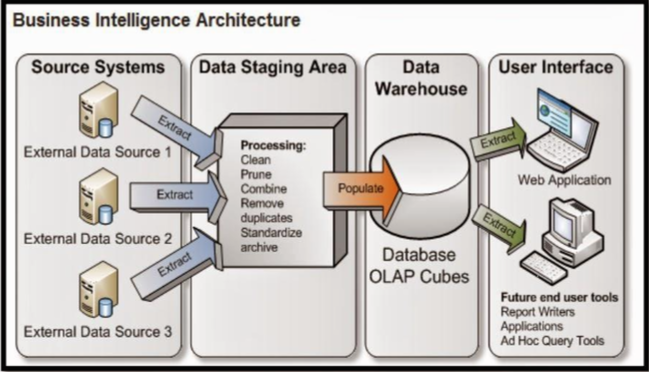
\includegraphics[scale=0.5]{Gambar/arsitektur-kecerdasan-bisnis.png}
	\caption[Arsitektur Kecerdasan Bisnis]{Arsitektur Kecerdasan Bisnis} 
	\label{fig:arsitektur_kecerdasan_bisnis_fig}
\end{figure}

Berdasarkan Gambar \ref{fig:arsitektur_kecerdasan_bisnis_fig} sistem kecerdasan bisnis terdiri dari empat tahap, yaitu:

\begin{enumerate}
	\item \textbf{Source Systems}\\
	\textit{Source systems} merupakan sumber data yang akan disimpan dan dimanfaatkan di sistem kecerdasaan bisnis. Data yang menjadi masukan sangat bermacam-macam. Data dapat berupa data terstruktur seperti basis data relasional, data excel, dan lain-lain. Data juga dapat berupa data yang tidak terstruktur seperti file teks, pesan dari sosial media, gambar, video dan lain-lain.
	
	\item \textbf{Data Staging Area}\\
	Data yang didapat dari berbagai sumber dengan format dan bentuk yang berbagai macam mengakibatkan perlunya pra pengolahan data terlebih dahulu agar mendapatkan data yang sesuai dan siap dimasukan ke dalam \textit{data warehouse}. Pra pengolahan data ini dilakukan di tempat penampungan data sementara yang biasanya disebut \textit{staging area}. Proses pra pengolahan data di \textit{staging area} terdiri dari ETCL (\textit{Extract Trasnform Cleaning and Load}).
		\begin{itemize}
			\item \textit{Extract} adalah proses pemilihan data-data yang dirasa perlu untuk diolah dan dianalisis. Proses \textit{Extract} ini diperlukan karena sumber data yang digunakan dapat sangat banyak dan besar namun tidak seluruh data tersebut dapat dimanfaatkan, sehingga diperlukan pemilihan data-data yang diperlukan saja agar dapat bermanfaat dan menghemat waktu pemrosesan.
			\item \textit{Transform} adalah proses mengubah bentuk data yang sudah ada ke dalam bentuk yang standar sesuai dengan kebutuhan di \textit{data warehouse}. Proses \textit{transform} ini diperlukan karena data yang diambil dari berbagai sumber kemungkinan memiliki standarisasi yang berbeda pula.
			\item \textit{Cleaning} adalah proses pembersihan data-data yang didapat agar hasil keluaran dari sistem kecerdasan bisnis yang dibuat dapat lebih baik kualitasnya.
			\item \textit{Load} adalah proses mengirimkan data-data hasil pembersihan ke dalam \textit{data warehouse}.
		\end{itemize}
	
	\item \textbf{Data Warehouse}
		
	
	\item \textbf{User Interface}
\end{enumerate} 


\subsection{Sentimen Analisis dalam Sistem Kecerdasan Bisnis}
\label{sec:sentimen_analisis}
Sentimen analisis mengacu pada bidang yang luas dari pengolahan bahasa alami, komputasi linguistik dan text mining yang bertujuan menganalisis pendapat, sentimen, evaluasi, sikap, penilaian dan emosi seseorang apakah pembicara atau penulis berkenaan dengan suatu topik, produk, layanan, organisasi, individu, ataupun kegiatan tertentu. \cite{liu2012sentiment} Hasil dari sentimen analisis berupa kelompok teks dengan nilai sentimen positif, netral atau negatif pada suatu objek tertentu.

\section{Sosial Media Twitter}
\label{sec:twitter}
Twitter adalah sebuah situs web yang dimiliki dan dioperasikan oleh Twitter Inc.. Twitter menawarkan jaringan sosial mikroblog dengan panjang pesan maksimal hingga 140 karakter, yang biasanya disebut Tweet. Melalui mikroblog Twitter, pengguna dapat memperbarui status terbaru tentang hal yang sedang mereka pikirkan ataupun berpendapat tentang suatu objek atau fenomena tertentu. Pesan yang dibuat pengguna akan tampil secara langsung dan dapat dilihat seluruh dunia melalui website Twitter atau berbagai aplikasi eksternal lainnya. Untuk menghemat karakter pada sebuah tweet biasanya pengguna menuliskan singkatan, bahasa slang atau emoticon dalam mengkomunikasikan pesannya. 

Pengguna Twitter dapat mengelompokan tweetnya dengan menggunakan hastags - kata atau frasa yang diawali dengan tanda "\#". Selain itu pengguna juga dapat menunjuk pengguna lainnya dengan menuliskan username mereka diawali dengan tanda "@". Setiap tweet yang dibuat dapat dibalas ataupun di tweet ulang (re-tweet) oleh pengguna lainnya.

\subsection{Twitter Streaming API}
\label{sec:twitter_streaming_api}
Twitter menyediakan Streaming API yang memudahkan pengembang aplikasi untuk mendapatkan tweet-tweet yang dibuat pengguna Twitter secara realtime. Streaming API yang tersedia memiliki beberapa jenis sesuai dengan kegunaannya, yaitu:

\begin{enumerate}
	\item \textbf{Public Streams}: Untuk melakukan streaming pada data publik secara realtime. Cocok untuk digunakan pada pencarian tweet berdasarkan user atau topik tertentu dan data mining.
	\item \textbf{User Streams}: Untuk melakukan streaming pada single-user, hasil streaming terdiri dari data-data yang berkaitan dengan kegiatan single-user.
	\item	\textbf{Site Streams}: Merupakan versi multi-user dari User Streams. Site Streams dimaksudkan untuk server yang harus terhubung ke Twitter atas nama banyak pengguna.
\end{enumerate}

\begin{figure}
\centering
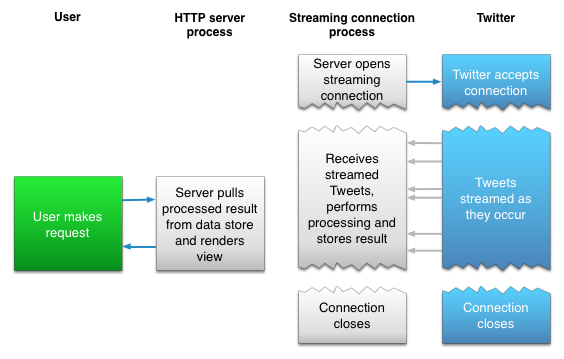
\includegraphics[scale=0.5]{Gambar/streaming-intro-2_1.png}
\caption[Proses Twitter Streaming API]{Proses Twitter Streaming API \cite{TwitterApi:2015}} 
\end{figure}

\section{Data Mining}
\label{sec:data_mining}
\subsection{Pengertian Data Mining}
Saat ini pertumbuhan informasi berkembang sangat cepat setiap harinya. Jutaan bahkan milyaran data dari proses bisnis, sosial, sains, dan hampir setiap aspek kehidupan kita dituangkan ke dalam berbagai perangkat penyimpanan data. Pertumbuhan data yang pesat dan penyimpanan dalam basis data yang besar dan banyak telah melampaui kemampuan manusia dalam memahami isi dari data tertsebut. Oleh karena itu data mining sangat diperlukan dalam menggali informasi atau pola yang terdapat di dalam tumpukan data yang sangat besar. Data-data yang akan ditambang dapat berasal dari basis data relasional, data warehouse, transactional database, advanced database system, flat file, data stream, text or multimedia. \cite{han2011data} 

\subsection{Proses \textit{Knowledge Discovery}}
Proses \textit{Knowledge Discovery} adalah proses pencarian pengetahuan pada data dapat berupa informasi atau pola. Dalam proses \textit{Knowledge Discovery} perlu dilakukan langkah-langkah seperti berikut.

\begin{enumerate}
	\item Data cleaning \\Proses pembersihan data yang kotor dan tidak konsisten.
	\item Data integration \\Proses untuk menyatukan data-data dari berbagai sumber lainnya.
	\item Data selection \\Proses pemilihan data yang relevan dengan analisis yang diambil dari basis data.
	\item Data transformation \\Proses perubahan data ke dalam bentuk yang sesuai untuk proses penambangan dengan melakukan ringkasan atau agregasi operasi.
	\item Data mining \\Proses dimana metode-metode diterapkan untuk mendapatkan informasi atau pola yang berguna.
	\item Pattern evaluation \\Proses melakukan evaluasi pada pola atau informasi yang diperoleh.
	\item Knowledge presentation \\Proses memvisualisasi pola atau informasi yang digunakan untuk menyajikan hasil penambangan kepada pengguna.
\end{enumerate}


\begin{figure}
\centering
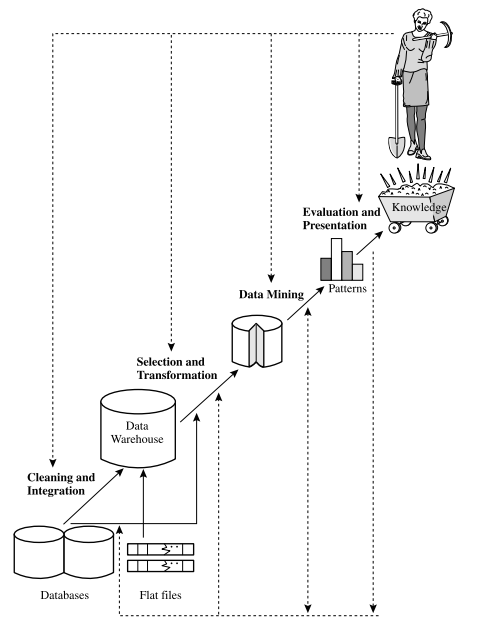
\includegraphics[scale=0.5]{Gambar/data-mini-process.png}
\caption[Step dalam melakukan Proses \textit{Knowledge Discovery}]{Step dalam melakukan Proses \textit{Knowledge Discovery} \cite{han2011data}} 
\end{figure}


\subsection{Teknik-Teknik Data Mining}
\begin{enumerate}
	\item \textit{Classification} (Pengklasifikasian)
	\textit{Classification} adalah proses menemukan fitur-fitur yang sama pada sebuah himpunan data di dalam basis data dan mengklasifikasikannya ke dalam kelas-kelas sesuai model klasifikasi yang ditetapkan. Proses \textit{Classification} terdiri dari dua langkah yaitu langkah pembelajaran (model klasifikasi dibangun) dan langkah klasifikasi (model digunakan untuk memprediksi kelas untuk data yang diberikan). Classification dikenal pula sebagai supervised learning di mana kelas-kelas telah didefinisikan sebelumnya.
	\item \textit{Clustering} (Pengelompokan)
	\textit{Clustering} adalah proses pengelompokan satu set benda-benda ke dalam kelas objek yang sama. Sebuah \textit{Cluster} adalah kumpulan objek data yang mirip satu sama lain dalam Cluster yang sama dan berbeda dengan benda-benda di cluster lain. Clustering dikenal juga sebagai unsupervised learning dimana kelas-kelas tidak diketahui sebelumnya. Clustering juga disebut segmentasi data dalam beberapa aplikasi karena mengelompokkan data set yang besar menjadi kelompok-kelompok yang memiliki kesamaan. 
	\item \textit{Regression} (Regresi)
	Regression hampir mirip dengan pengklasifikasian. Akan tetapi, Regression menggunakan nilai yang ada untuk memperkirakan nilai yang akan muncul kemudian. Cara untuk mengetahui ketepatan dari pengklasifikasian adalah dengan menggunakan \textit{wait} and \textit{see}.
\end{enumerate}

\section{Text Mining}
\label{sec:text_mining}

\subsection{Pengertian Text Mining}
Text mining adalah salah satu bidang khusus dari data mining. Text mining dapat didefinisikan sebagai suatu proses menggali informasi dimana seorang user berinteraksi dengan sekumpulan text menggunakan tools analisis yang merupakan komponen-komponen dalam data mining yang salah satunya adalah kategorisasi. \cite{feldman2006j} Tujuan dari text mining adalah untuk mendapatkan informasi yang berguna dari sekumpulan text. Sumber data yang digunakan pada text mining adalah kumpulan text yang memiliki format yang tidak terstruktur atau minimal semi terstruktur. Adapun tugas khusus dari text mining antara lain yaitu pengkategorisasian text (\textit{text categorization}) dan pengelompokan text (\textit{text clustering}).

Permasalahan yang dihadapi pada text mining sama dengan permasalahan yang terdapat pada data mining, yaitu jumlah data yang besar, dimensi yang tinggi, data dan struktur yang terus berubah, dan data \textit{noise}. Perbedaan di antara keduanya adalah pada data yang digunakan. Pada data mining, data yang digunakan adalah data terstruktur, sedangkan pada text mining, data yang digunakan pada umumnya adalah data tidak terstruktur atau minimal semiterstruktur. Hal ini menyebabkan adanya tantangan tambahan pada text mining yaitu struktur text yang kompleks dan tidak lengkap, arti yang tidak jelas serta tidak umum, dan bahasa yang berbeda-beda.

\subsection{Proses Text Mining}
\begin{figure}
\centering
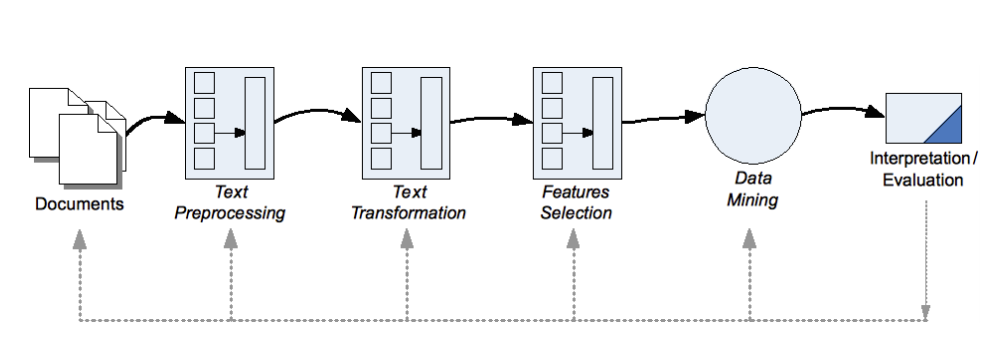
\includegraphics[scale=0.5]{Gambar/proses-text-mining.png}
\caption[Proses Text Mining]{Proses Text Mining.\\Sumber: http://lecturer.ukdw.ac.id/budsus/pdf/textwebmining/TextMining\_Kuliah.pdf} 
\end{figure}

Proses-proses yang umumnya dilakukan dalam melakukan Text Mining adalah

\begin{enumerate}
	\item Text Preprocessing\\
	Tahap text preprocessing adalah tahap awal dari text mining. Tahap ini mencakup semua rutinitas, dan proses untuk mempersiapkan data yang akan digunakan pada operasi \textit{knowledge discovery} sistem text mining. \cite{feldman2007text}. Biasanya pada proses ini text akan diubah ke dalam huruf kecil lalu terjadi pembuangan delimiter-delimiter seperti tanda baca.
	
	\item Text Transformation\\
	Pada tahap ini teks akan diubah bentuknya sesuai dengan kebutuhan proses penambangan.
	
	\item Feature Selection\\
	Tahap seleksi fitur (feature selection) bertujuan untuk mengurangi dimensi dari suatu kumpulan teks, atau dengan kata lain menghapus kata-kata yang dianggap tidak penting atau tidak menggambarkan isi dokumen sehingga proses pengklasifikasian lebih efektif dan akurat. \cite{manalu2014analisis}. Pada tahap ini tindakan yang dilakukan adalah menghilangkan \textit{stopword} (\textit{stopword removal}) dan \textit{stemming} terhadap kata yang berimbuhan.\cite{berry2010text}
	
	\textit{Stopword} adalah kosakata yang bukan merupakan ciri dari suatu teks. Misalnya "di", "oleh", "pada", "selama", "sebab" dan lain sebagainya. Sebelum proses \textit{stopword removal} dilakukan, harus dibuat daftar stopword (stoplist). Jika termasuk di dalam stoplist maka kata-kata tersebut akan dihapus dari deskripsi sehingga kata-kata yang tersisa di dalam deskripsi dianggap sebagai kata-kata yang mencirikan isi dari suatu dokumen atau keywords. Daftar kata stopword di penelitian ini bersumber dari Tala (2003) \cite{tala2003study}.
	
	Setelah melalui proses \textit{stopword removal} langkah berikutnya adalah proses \textit{stemming}. \textit{Stemming} adalah proses pemetaan dan penguraian berbagai bentuk (variants) dari suatu kata menjadi bentuk kata dasarnya (stem) \cite{tala2003study}. Tujuan dari proses ini adalah untuk menghilangkan imbuhan-imbuhan baik itu berupa prefiks, sufiks, maupun konfiks yang ada pada setiap kata. \cite{manalu2014analisis} Dengan adanya proses stemming ini maka dimensi data akan berkurang sehingga data dapat diproses dengan lebih cepat dan akurat.
\end{enumerate}

\section{Hadoop}
\label{sec:hadoop}

\subsection{Pengertian Hadoop}
\label{sec:pengertian_hadoop}
Apache Hadoop adalah sebuah \textit{framework opensource} yang memungkinkan untuk memproses set data yang besar secara terdistribusi di \textit{cluster} komputer menggunakan model pemrograman yang sederhana. Hadoop dirancang untuk mendeteksi dan menangani kegagalan pada lapisan aplikasi, sehingga memberikan layanan yang \textit{highly-available} pada sekelompok komputer yang masing-masingnya mungkin rentan terhadap kegagalan. Hal tersebut lebih baik dibanding hanya mengandalkan perangkat keras untuk memberikan \textit{high-availability}.

Hadoop bekerja dengan menggunakan penyimpanan terdistribusi dan mentransfer kode program bukan datanya. Hadoop menghindari langkah transmisi yang mahal ketika bekerja dengan kumpulan data besar. Selain itu, redundansi data pada Hadoop memungkinkan Hadoop untuk memulihkan \textit{single node} yang gagal. Anda akan mendapatkan kemudahan membuat program dengan Hadoop menggunakan MapReduce \textit{framework}. Yang juga tak kalah penting adalah Anda tidak perlu khawatir tentang cara melakukan partisi data, menentukan node yang akan melakukan tugas, atau menangani komunikasi antar node. Hadoop menangani ini untuk Anda, sehingga Anda dapat fokus pada apa yang paling penting bagi data Anda dan apa yang ingin Anda lakukan dengan itu.

\subsection{Komponen Utama Hadoop}
\label{sec:komponen_utama_hadoop}
\begin{figure}
	\centering
	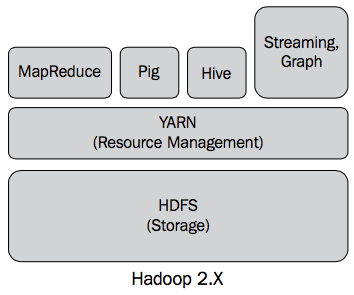
\includegraphics[scale=0.5]{Gambar/hadoop-architecture.png}
	\caption[Arsitektur Komponen Hadoop]{Arsitektur Komponen Hadoop.\cite{holmes2012hadoop}} 
	\label{fig:komponen_utama_hadoop}
\end{figure}

Gambar \ref{fig:komponen_utama_hadoop} menjelas tentang arsitektur Hadoop. Terdapat HDFS, YARN dan MapReduce yang menjadi komponen dasar pembentuk Hadoop. Di bagian atasnya terdapat ekosistem lainnya yang dapat berjalan di atas Hadoop.

\subsubsection{Hadoop Distributed File System (HDFS)}
HDFS adalah sebuah file sistem yang didesain untuk memproses data distribusi skala besar di dalam framwork seperti MapReduce. HDFS dapat menyimpan sebuat data set sebesar 100TB sebagai sebuah single file.\cite{Lam:2010:HA:1965594} HDFS bisa bersifat single node atau multiple node. HDFS bukan native File System seperti layaknya EXT3, EXT4, FAT atau NTFS. HDFS ada pada layer di atasnya.

HDFS menyimpan suatu data dengan cara membelahnya menjadi potongan-potongan data yang berukuran 64 MB, dan potongan-potongan data ini kemudian disimpan tersebar dalam komputer-komputer yang membentuk clusternya. Potongan-potongan data tersebut dalam HDFS disebut block, dan ukurannya tidak terpaku harus 64 MB. Ukuran block dapat diatur sesuai kebutuhan 128MB, 256MB ataupun 1GB.

Walaupun data disimpan secara tersebar, dari kacamata pengguna, data tetap terlihat seperti halnya kita mengakses file pada satu komputer. File yang secara fisik disimpan tersebar dalam banyak komputer itu pun dapat diperlakukan layaknya memperlakukan file dalam satu komputer.

Sebagai distributed file system, HDFS memiliki komponen-komponen utama berupa NameNode dan DataNode seperti yang digambarkan pada Gambar \ref{fig:fig:hadoop-cluster}. NameNode adalah sebuah komputer yang bertindak sebagai master, sedangkan DataNode adalah komputer-komputer dalam Hadoop Cluster yang bertugas sebagai slaves. NameNode bertanggungjawab menyimpan informasi tentang penempatan block-block data dalam Hadoop Cluster. Ia memiliki JobTracker yang bertanggungjawab mengorganisir dan mengontrol block-block data yang disimpan tersebar dalam komputer-komputer yang menyusun Hadoop Cluster. Sedangkan DataNode dilengkapi dengan TaskTracker bertugas menyimpan block-block data yang dialamatkan kepadanya, dan secara berkala melaporkan kondisinya kepada NameNode. Laporan berkala DataNode kepada NameNode ini disebut Heartbeat. Berdasarkan Heartbeat ini NameNode dapat mengetahui dan menguasai kondisi cluster secara keseluruhan. Sebagai balasan atas Heartbeat dari DataNode, NameNode akan mengirimkan perintah kepada DataNode. Apabila terjadi kerusakan pada NameNode, maka Secondary NameNode akan langsung aktif dan bertugas sebagai pengganti NameNode.

Jadi, dalam HDFS, NameNode adalah bos yang mengatur dan mengendalikan Hadoop Cluster. Sedangkan, DataNode adalah pekerja yang bertugas menyimpan data dan melaksanakan perintah dari NameNode.

\begin{figure}
	\centering
	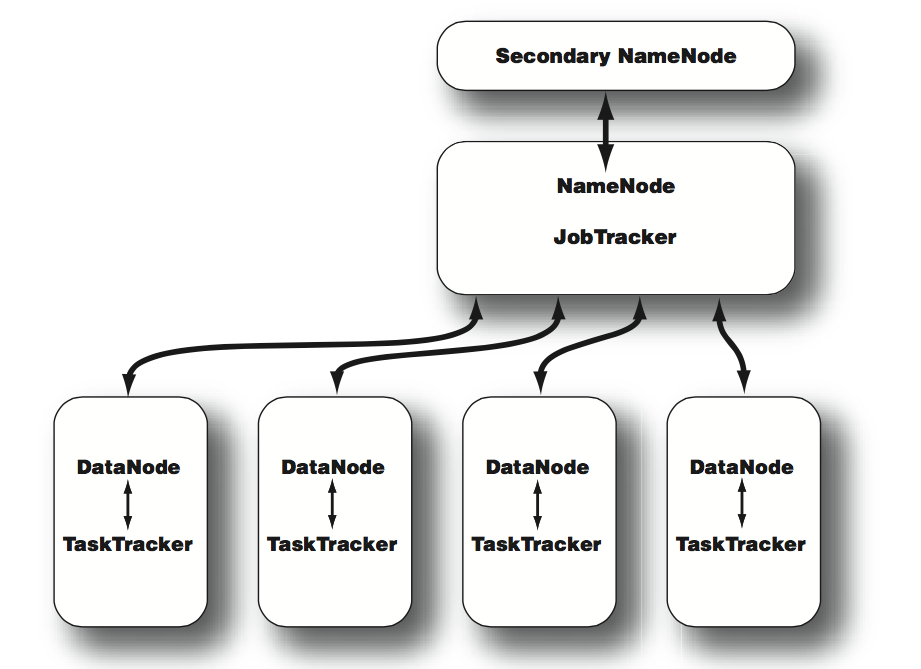
\includegraphics[scale=0.3]{Gambar/hadoop-cluster.png}
	\caption[Hadoop Cluster]{Hadoop Cluster.\cite{Lam:2010:HA:1965594}}
	\label{fig:hadoop-cluster}
\end{figure}
	
\subsubsection{Hadoop MapReduce}
\label{sec:hadoop_mapreduce}
MapReduce adalah sebuah model pemrosesan data\cite{Lam:2010:HA:1965594}. MapReduce ditujukan untuk memproses data berukuran raksasa secara terdistribusi dan paralel dalam cluster yang terdiri atas banyak komputer. Dalam memproses data, secara garis besar MapReduce dapat dibagi dalam dua proses yaitu proses \textit{Map} dan proses \textit{Reduce}. Kedua jenis proses ini didistribusikan ke setiap komputer nodes dalam suatu cluster (kelompok komputer yang saling terhubung) dan berjalan secara paralel tanpa saling bergantung satu dengan yang lainnya. Proses \textit{Map} bertugas untuk mengumpulkan informasi dari potongan-potongan data yang terdistribusi dalam tiap komputer dalam \textit{cluster}. Hasilnya diserahkan kepada proses \textit{Reduce} untuk diproses lebih lanjut. Hasil proses Reduce merupakan hasil akhir yang dikirim ke pengguna. \cite{Dean:2008:MSD:1327452.1327492}

MapReduce menggunakan tipe data \textit{list} dan \textit{(key/value) pairs} sebagai data primitif utamanya. \textit{Keys} dan \textit{values} biasanya berupa integer atau string tapi bisa juga menggunakan \textit{dummy value} atau objek data lainnya. Oleh karena itu fungsi \textit{map} dan \textit{reduce} harus bisa menangani berbagai data tersebut.

Di dalam \textit{framework} MapReduce, aplikasi ditulis dengan memspesifikasikan \textit{mapper} dan \textit{reducer}. Berikut adalah contoh lengkap aliran data yang terjadi pada MapReduce.

\begin{table}
	\centering
	\begin{tabular}{l | c | c}
		 & Input & Output \\
	 	\hline
		map & <k1, v1> & list(<k2, v2>) \\
		reduce & <k3, list(v2)> & list(<k3, v3>) \\ 
		\label{tab:mapreduce_process}
	\end{tabular}	
	\caption{Input dan Output pada MapReduce}
\end{table}	

\begin{enumerate}
	\item Masukan data ke dalam aplikasi harus terstruktur dalam bentuk \textit{lists} dari \textit{(key/value) pairs}, list(<k1, v1>). Dalam pengaplikasiannya input dapat dibuat seperti contoh berikut, list(<String filename, String filecontent>) atau list(<Integer messageid, String message>).
	\item Setelah masukan diterima maka proses mapper akan dijalankan. Proses mapper akan membagi masukan \textit{lists} dari \textit{(key/value) pairs} menjadi masing-masing \textit{(key/value) pairs}, <k1, v1>. \textit{Mapper} mengubah setiap <k1, v1> dan memasangkannya menjadi list(<k2, v2>) secara acak. Pada contoh kasus penghitung kata, mapper mendapatkan masukan berupa list(<String filename, String filecontent>), kemudian \textit{list} dipecah menjadi <String filename, String filecontent> \textit{pairs}. Teks yang terdapat pada filecontent dihitung satu per satu yang akan menghasilkan keluaran berupa <String word, Integer count>, contoh: <"hello", 1>, <"hello", 2>, <"world", 1>. 
	\item Seluruh keluaran yang dihasilkan dari proses Mapper dikumpulkan dan menjadi sebuah \textit{list of <k2, v2> pairs} raksasa. Semua pasangan yang memiliki nilai k2 yang sama akan dikelompokan menjadi satu pasangan baru yaitu <k2, list(v2)>. Kemudian \textit{framework} akan menjalakan fungsi \textit{reducer} untuk memproses masing-masing pasangan baru menjadi list(<k3, v3>). Pada contoh kasus penghitung kata, misal ada pasangan <"hello", 1> sebanyak dua buah, maka reducer akan memprosesnya menjadi <"hello", list(1,1)> dan keluaran yang dihasilkan oleh reducer akan menjadi <"hello", 2>. Hasil dari masing-masing pasangan akan disatukan kembali dalam bentuk list, misal list(<"hello", 2>, <"world", 1>).
\end{enumerate} 

Gambar \ref{fig:mapper_works} menggambarkan cara kerja Map pada HDFS. 
\begin{enumerate}
	\item Masukan data berukuran besar dari pesan, log, sensor, dsb ke dalam HDFS yang dibagi ke dalam beberapa block data, kemudian dibagi ke dalam \textit{record-record}.
	\item Data yang sudah dibagi-bagi ke DataNode melakukan tugas Map. 
	\item Keluaran yang dihasilkan diurutkan dan akan menjadi masukan bagi reducer.
\end{enumerate}


\begin{figure}
	\centering
	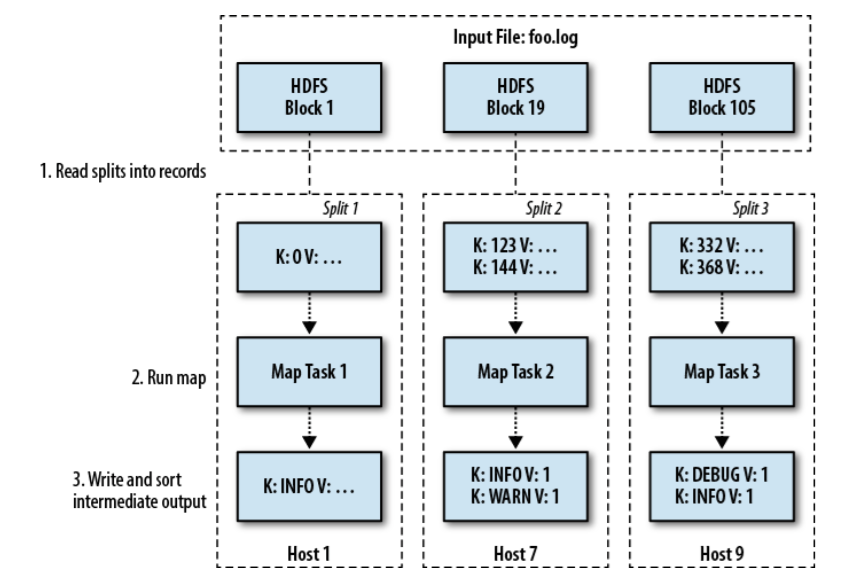
\includegraphics[scale=0.5]{Gambar/how-mapper-works.png}
	\caption[Cara  Kerja Map]{Cara Kerja Map.\cite{sammer2012hadoop}}
	\label{fig:mapper_works}
\end{figure}

Gambar \ref{fig:reducer_works} menggambarkan cara kerja Reduce pada HDFS.
\begin{enumerate}
	\item Masukan data dari hasil fungsi mapper.
	\item Menjalankan fungsi reduce untuk menyatukan data kembali.
	\item Keluaran yang dihasilkan disimpan kembali ke dalam HDFS.
\end{enumerate}

\begin{figure}
	\centering
	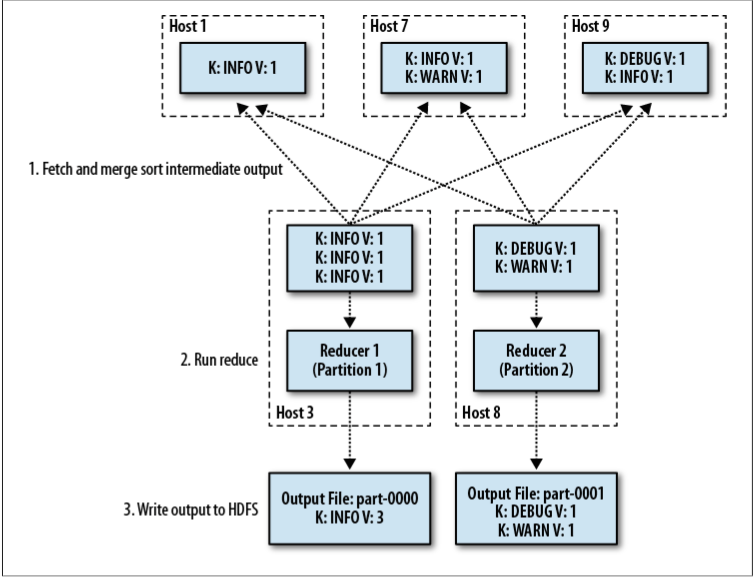
\includegraphics[scale=0.5]{Gambar/how-reducer-works.png}
	\caption[Cara  Kerja Reduce]{Cara Kerja Reduce.\cite{sammer2012hadoop}}
	\label{fig:reducer_works}
\end{figure}
	
\subsubsection{Hadoop YARN}
Hadoop Yet Another Resource Negotiator atau YARN adalah teknologi untuk mengatur \textit{resource} dan \textit{scheduling} pada sebuah cluster. YARN berada suatu layer diatas HDFS yang memungkinkan aplikasi lain untuk memproses data yang sama di Hadoop secara paralel dengan MapReduce. Pada Hadoop versi 2.x MapReduce dianggap sebuah aplikasi YARN.

\subsection{Hive}
\label{sec:hive}
Apache Hive adalah perangkat lunak \textit{data warehouse} yang memfasilitasi kueri dan mengelola dataset besar yang berada dalam penyimpanan terdistribusikan. Apache Hive dibangun dan berjalan di atas Apache Hadoop. Pada awalnya Hive dibuat oleh Facebook untuk memproses data user dan log yang sangat besar. Saat ini Hive sudah menjadi proyek \textit{open source} dengan banyak kontributor dan merupakan subproyek dari Hadoop.  

Target dari pengguna Hive adalah para data analis yang terbiasa menggunakan SQL dalam pekerjaannya. Hive mendefinisikan sebuah SQL sederhana seperti bahasa kueri yang disebut HiveQL. HiveQL memungkingkan pengguna yang terbiasa dengan SQL untuk melakukan kueri pada data. Dengan menggunakan Hive para pengguna dapat melakukan kueri-kueri untuk \textit{summarization} dan data analisis pada lingkungan data Hadoop. 

HiveQL terinspirasi untuk memisahkan bahasa yang digunakan pengguna dengan kompleksitas MapReduce. HiveQL menggunakan kembali konsep dari \textit{database} relasional, seperti tabel, baris, kolom, dan skema, untuk memudahkan pembelajaran. Namun perlu diingat karena Hive dibangun di atas Hadoop dan sifatnya yang dirancang untuk tipe \textit{batch oriented} dalam pemrosesan datanya, maka Hive bukanlah pengganti langsung untuk data warehouse SQL tradisional.

Hive memiliki sedikit perbedaan dengan Hadoop dalam penyimpanan datanya. Di Hadoop data disimpan dalam bentuk flat file, sedangkan di Hive data dapat menggunakan direktori untuk melakukan partisi data. Dengan adanya partisi pada data di Hive, maka proses pencarian dapat dilakukan dengan lebih baik daripada disimpan dalam bentuk flat file. Untuk mendukung fitur-fitur tambahan ini, Hive memerlukan komponen tambahan seperti metastore. Metastore berfungsi untuk menyimpan informasi skema. Metastore ini biasanya berada dalam database relasional. Metastore disimpan di dalam sebuah direktori di dalam Hive.

Pengguna dapat berinteraksi dengan Hive menggunakan beberapa metode, termasuk GUI Web dan Java Database Connectivity (JDBC). Gambar \ref{fig:hive_architecture} menggambarkan sebuah diagram \textit{high level} arsitektur dari Hive. Pada arsitektur Hive kueri dipecah dan dijalankan pada Hadoop. Metastore merupakan komponen penting yang membantu menentukan bagaimana kueri akan dijalankan pada Hive.

\begin{figure}
	\centering
	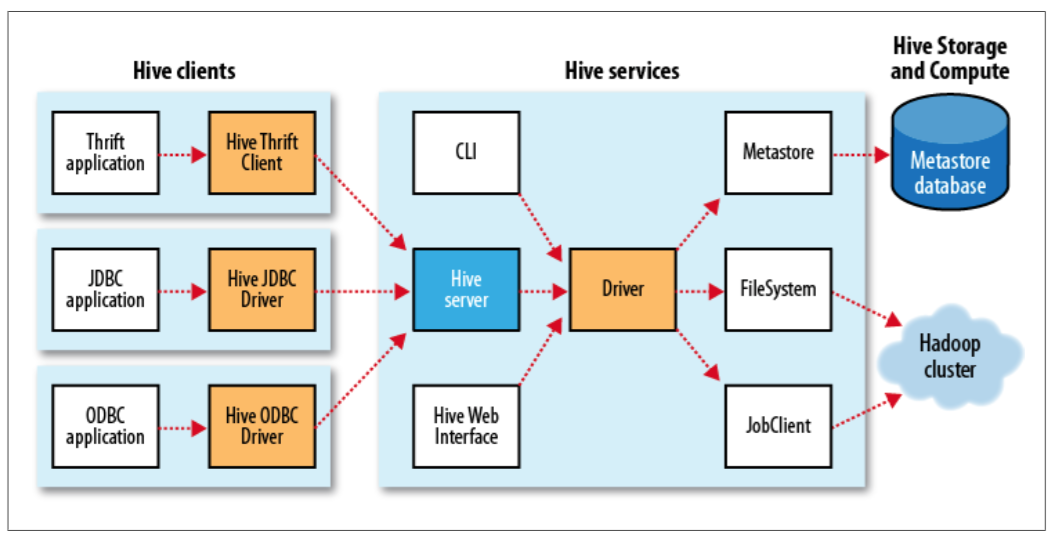
\includegraphics[scale=0.5]{Gambar/arsitektur-hive.png}
	\caption[Arsitektur Hive]{Arsitektur Hive} 
	\label{fig:hive_architecture}
\end{figure}

\subsubsection{DDL Operation Hive}
Seperti layaknya sebuah SQL tradisional, Hive memiliki fungsi-fungsi Data Definition Language (DDL) yang dapat digunakan untuk membantu pengguna dalam membuat dan mengelola tabel-tabel, view, index ataupun function. Berikut adalah \textit{statement} DDL yang dapat digunakan oleh pengguna.

\begin{itemize}
	\item CREATE DATABASE/SCHEMA, TABLE, VIEW, FUNCTION, INDEX
	\item DROP DATABASE/SCHEMA, TABLE, VIEW, INDEX
	\item TRUNCATE TABLE
	\item ALTER DATABASE/SCHEMA, TABLE, VIEW
	\item MSCK REPAIR TABLE (or ALTER TABLE RECOVER PARTITIONS)
	\item SHOW DATABASES/SCHEMAS, TABLES, TBLPROPERTIES, PARTITIONS, FUNCTIONS, INDEX, COLUMNS, CREATE TABLE
	\item DESCRIBE DATABASE SCHEMA
\end{itemize}

Berikut adalah \textit{keyword-keyword} yang dapat digunakan (Non-reserved) di dalam Hive.

\begin{lstlisting}[basicstyle=\tiny,caption=Non-reserved Keywords]
ADD, ADMIN, AFTER, ANALYZE, ARCHIVE, ASC, BEFORE, BUCKET, BUCKETS, CASCADE, CHANGE, CLUSTER, 
CLUSTERED, CLUSTERSTATUS, COLLECTION, COLUMNS, COMMENT, COMPACT, COMPACTIONS, COMPUTE, 
CONCATENATE, CONTINUE, DATA, DATABASES, DATETIME, DAY, DBPROPERTIES, DEFERRED, DEFINED, 
DELIMITED, DEPENDENCY, DESC, DIRECTORIES, DIRECTORY, DISABLE, DISTRIBUTE, ELEM_TYPE, ENABLE, 
ESCAPED, EXCLUSIVE, EXPLAIN, EXPORT, FIELDS, FILE, FILEFORMAT, FIRST, FORMAT, FORMATTED, 
FUNCTIONS, HOLD_DDLTIME, HOUR, IDXPROPERTIES, IGNORE, INDEX, INDEXES, INPATH, INPUTDRIVER, 
INPUTFORMAT, ITEMS, JAR, KEYS, KEY_TYPE, LIMIT, LINES, LOAD, LOCATION, LOCK, LOCKS, LOGICAL, LONG, 
MAPJOIN, MATERIALIZED, MINUS, MINUTE, MONTH, MSCK, NOSCAN, NO_DROP, OFFLINE, OPTION, OUTPUTDRIVER, 
OUTPUTFORMAT, OVERWRITE, OWNER, PARTITIONED, PARTITIONS, PLUS, PRETTY, PRINCIPALS, PROTECTION, 
PURGE, READ, READONLY, REBUILD, RECORDREADER, RECORDWRITER, REGEXP, 
RELOAD, RENAME, REPAIR, REPLACE, RESTRICT, REWRITE, RLIKE, ROLE, ROLES, 
SCHEMA, SCHEMAS, SECOND, SEMI, SERDE, SERDEPROPERTIES, SERVER, SETS, SHARED, SHOW, SHOW_DATABASE, 
SKEWED, SORT, SORTED, SSL, STATISTICS, STORED, STREAMTABLE, STRING, STRUCT, TABLES, TBLPROPERTIES, 
TEMPORARY, TERMINATED, TINYINT, TOUCH, TRANSACTIONS, UNARCHIVE, UNDO, UNIONTYPE, UNLOCK, UNSET, 
UNSIGNED, URI, USE, UTC, UTCTIMESTAMP, VALUE_TYPE, VIEW, WHILE, YEAR
\end{lstlisting}

Berikut adalah \textit{keyword-keyword} yang tidak dapat digunakan secara langsung (Reserved) di dalam Hive. \textit{Reserved keyword}  ini sebaiknya dihindari penggunaannya dalam menuliskan kueri-kueri Hive. Namun apabila tetap diperlukan maka untuk menggunakan \textit{reserved keyword} dapat menambahkan \textit{quoted identifier} atau mengatur parameter konfigurasi dari Hive (set hive.support.sql11.reserved.keywords=false)

\begin{lstlisting}[basicstyle=\tiny,caption=Reserved Keywords]
ALL, ALTER, AND, ARRAY, AS, AUTHORIZATION, BETWEEN, BIGINT, BINARY, BOOLEAN, BOTH, BY, CASE, CAST, 
CHAR, COLUMN, CONF, CREATE, CROSS, CUBE, CURRENT, CURRENT_DATE, CURRENT_TIMESTAMP, CURSOR, 
DATABASE, DATE, DECIMAL, DELETE, DESCRIBE, DISTINCT, DOUBLE, DROP, ELSE, END, EXCHANGE, EXISTS, 
EXTENDED, EXTERNAL, FALSE, FETCH, FLOAT, FOLLOWING, FOR, FROM, FULL, FUNCTION, GRANT, GROUP, 
GROUPING, HAVING, IF, IMPORT, IN, INNER, INSERT, INT, INTERSECT, INTERVAL, INTO, IS, JOIN, LATERAL, 
LEFT, LESS, LIKE, LOCAL, MACRO, MAP, MORE, NONE, NOT, NULL, OF, ON, OR, ORDER, OUT, OUTER, OVER, 
PARTIALSCAN, PARTITION, PERCENT, PRECEDING, PRESERVE, PROCEDURE, RANGE, READS, REDUCE, 
REGEXP (Hive 2.0.0 onward), REVOKE, RIGHT, RLIKE (Hive 2.0.0 onward), ROLLUP, ROW, ROWS, 
SELECT, SET, SMALLINT, TABLE, TABLESAMPLE, THEN, TIMESTAMP, TO, TRANSFORM, TRIGGER, TRUE, 
TRUNCATE, UNBOUNDED, UNION, UNIQUEJOIN, UPDATE, USER, USING, VALUES, VARCHAR, WHEN, WHERE, 
WINDOW, WITH
\end{lstlisting}

Berikut adalah format-format dan contoh-contoh DDL pada Hive.

\begin{lstlisting}[language=sql,basicstyle=\tiny,caption=DDL untuk create database]
CREATE (DATABASE|SCHEMA) [IF NOT EXISTS] database_name
  [COMMENT database_comment]
  [LOCATION hdfs_path]
  [WITH DBPROPERTIES (property_name=property_value, ...)];
\end{lstlisting}

\begin{lstlisting}[language=sql,basicstyle=\tiny,caption=DDL untuk drop database]
DROP (DATABASE|SCHEMA) [IF EXISTS] database_name [RESTRICT|CASCADE];
\end{lstlisting}

\begin{lstlisting}[language=sql,basicstyle=\tiny,caption=DDL untuk alter database]
ALTER (DATABASE|SCHEMA) database_name SET DBPROPERTIES (property_name=property_value, ...);   -- (Note: SCHEMA added in Hive 0.14.0)
ALTER (DATABASE|SCHEMA) database_name SET OWNER [USER|ROLE] user_or_role;   -- (Note: Hive 0.13.0 and later; SCHEMA added in Hive 0.14.0)
\end{lstlisting}

\begin{lstlisting}[language=sql,basicstyle=\tiny,caption=DDL untuk use database]
USE database_name;
USE DEFAULT;
\end{lstlisting}

\begin{lstlisting}[language=sql,basicstyle=\tiny,caption=Contoh DDL untuk membuat tabel dengan partisi]
create table table_name (
  id			int,
  dtDontQuery	string,
  name			string
)
partitioned by (date string)
\end{lstlisting}

\begin{lstlisting}[language=sql,basicstyle=\tiny,caption=Contoh DDL untuk drop tabel]
DROP TABLE [IF EXISTS] table_name [PURGE];     -- (Note: PURGE available in Hive 0.14.0 and later)
\end{lstlisting}

\subsubsection{DML Operation Hive}
Data Manipulation Languange (DML) digunakan untuk melakukan kueri-kueri terhadap isi data dari suatu tabel. Pada Hive ada beberapa operasi dalam melakukan manipulasi data seperti load, insert, update, dan delete. 

\textbf{Load}\\
Pada proses load Hive tidak melakukan transformasi data apapun. Proses ini murni hanya untuk melakukan operasi copy/move data files ke dalam lokasi yang sesuai pada tabel Hive. Berikut syntax dari proses load pada Hive.

\begin{lstlisting}[language=sql,basicstyle=\tiny,caption=Syntax DML Load]
LOAD DATA [LOCAL] INPATH 'filepath' [OVERWRITE] INTO TABLE tablename [PARTITION (partcol1=val1, partcol2=val2 ...)]
\end{lstlisting}

\begin{lstlisting}[language=sql,basicstyle=\tiny,caption=Contoh DML Load]
LOAD DATA INPATH '/user/myname/kv2.txt' OVERWRITE INTO TABLE invites PARTITION (ds='2008-08-15');
\end{lstlisting}

\textbf{Penjelasan: }
\begin{itemize}
	\item \textit{filepath} dapat berupa:
		\begin{itemize}
			\item sebuah \textit{relative path}, seperti project/data1
			\item sebuah \textit{absolut path}, seperti /user/hive/project/data1
			\item sebuah \textit{full URI}, seperti hdfs://namenode:9000/user/hive/project/data1
		\end{itemize}
	\item Target yang dimasukan dapat berupa tabel atau partisi. Jika tabel dipartisi, maka harus menentukan partisi tertentu dari tabel yang akan dimuat berupa nilai dari seluruh kolom yang dipartisi.
	\item Keyword LOCAL sifatnya adalah optional, jika digunakan maka yang akan terjadi adalah perintah load akan melihat \textit{filepath} di the local file system. Namun jika keyword LOCAL tidak digunakan maka yang akan terjadi adalah Hive akan menggunakan URI \textit{filepath} lengkap.
\end{itemize}

Beberapa catatan yang perlu diingat dalam menggunakan kueri load ini adalah
\begin{itemize}
	\item \textit{filepath} tidak boleh terdiri dari sub direktori
	\item Jika \textit{keyword} LOCAL tidak digunakan, \textit{filepath} harus mengacu ke file dalam \textit{filesystem} yang sama dengan tabel atau partisi.
\end{itemize}

\textbf{Insert}\\
Perintah insert berfungsi untuk memasukan data ke dalam tabel pada Hive. Syntax kueri insert pada Hive memiliki \textit{standard syntax, multiple insert dan dynamic partition insert}. Standard syntax merupakan kueri dasar dari insert dalam melakukan input data ke dalam sebuah tabel. Multiple insert digunakan untuk melakukan proses input data ke dalam beberapa tabel sekaligus. Sedangkan dynamic partition insert digunakan untuk melakukan input data menggunakan partisi.

\begin{lstlisting}[language=sql,basicstyle=\tiny,caption=Syntax DML Insert]
Standard syntax:
INSERT OVERWRITE TABLE tablename1 [PARTITION (partcol1=val1, partcol2=val2 ...) [IF NOT EXISTS]] select_statement1 FROM from_statement;
INSERT INTO TABLE tablename1 [PARTITION (partcol1=val1, partcol2=val2 ...)] select_statement1 FROM from_statement;
 
Hive extension (multiple inserts):
FROM from_statement
INSERT OVERWRITE TABLE tablename1 [PARTITION (partcol1=val1, partcol2=val2 ...) [IF NOT EXISTS]] select_statement1
[INSERT OVERWRITE TABLE tablename2 [PARTITION ... [IF NOT EXISTS]] select_statement2]
[INSERT INTO TABLE tablename2 [PARTITION ...] select_statement2] ...;
FROM from_statement
INSERT INTO TABLE tablename1 [PARTITION (partcol1=val1, partcol2=val2 ...)] select_statement1
[INSERT INTO TABLE tablename2 [PARTITION ...] select_statement2]
[INSERT OVERWRITE TABLE tablename2 [PARTITION ... [IF NOT EXISTS]] select_statement2] ...;
 
Hive extension (dynamic partition inserts):
INSERT OVERWRITE TABLE tablename PARTITION (partcol1[=val1], partcol2[=val2] ...) select_statement FROM from_statement;
INSERT INTO TABLE tablename PARTITION (partcol1[=val1], partcol2[=val2] ...) select_statement FROM from_statement;
\end{lstlisting}

\begin{lstlisting}[language=sql,basicstyle=\tiny,caption=Contoh DML Insert]
INSERT OVERWRITE TABLE events SELECT a.* FROM profiles a;
INSERT OVERWRITE TABLE events SELECT a.* FROM profiles a WHERE a.key < 100;
INSERT OVERWRITE LOCAL DIRECTORY '/tmp/reg_3' SELECT a.* FROM events a;
INSERT OVERWRITE DIRECTORY '/tmp/reg_4' select a.invites, a.pokes FROM profiles a;
INSERT OVERWRITE DIRECTORY '/tmp/reg_5' SELECT COUNT(*) FROM invites a WHERE a.ds='2008-08-15';
INSERT OVERWRITE DIRECTORY '/tmp/reg_5' SELECT a.foo, a.bar FROM invites a;
INSERT OVERWRITE LOCAL DIRECTORY '/tmp/sum' SELECT SUM(a.pc) FROM pc1 a;
FROM invites a INSERT OVERWRITE TABLE events SELECT a.bar, count(*) WHERE a.foo > 0 GROUP BY a.bar;
FROM pokes t1 JOIN invites t2 ON (t1.bar = t2.bar) INSERT OVERWRITE TABLE events SELECT t1.bar, t1.foo, t2.foo;

//Multitable insert
FROM src
INSERT OVERWRITE TABLE dest1 SELECT src.* WHERE src.key < 100
INSERT OVERWRITE TABLE dest2 SELECT src.key, src.value WHERE src.key >= 100 and src.key < 200
INSERT OVERWRITE TABLE dest3 PARTITION(ds='2008-04-08', hr='12') SELECT src.key WHERE src.key >= 200 and src.key < 300
INSERT OVERWRITE LOCAL DIRECTORY '/tmp/dest4.out' SELECT src.value WHERE src.key >= 300;
\end{lstlisting}


%TODO: Penjelasan



\textbf{Update}\\
Perintah update berfungsi untuk melakukan perubahan data yang sudah ada pada tabel. Perintah update pada Hive cukup sederhana layaknya pada SQL syntax lainnya. 

\begin{lstlisting}[language=sql,basicstyle=\tiny,caption=Syntax DML Update]
UPDATE tablename SET column = value [, column = value ...] [WHERE expression]
\end{lstlisting}

\textbf{Penjelasan:}
\begin{itemize}
	\item \textit{Value} yang diberikan harus sebuah ekspresi yang dapat dilakukan oleh Hive. Sehingga operator aritmatika, cast, literal dll dapat digunakan. Tetapi nilai dari sub kueri tidak dapat digunakan dalam pemberian \textit{value}.
	\item Kolom yang dipartisi tidak dapat diperbaharui dengan perintah update.
\end{itemize}

\textbf{Delete}\\
Perintah delete berfungsi untuk melakukan penghapusan data yang sudah ada pada tabel. Perintah delete pada Hive cukup sederhana layaknya pada SQL syntax lainnya. 

\begin{lstlisting}[language=sql,basicstyle=\tiny,caption=Syntax DML Delete]
DELETE FROM tablename [WHERE expression]
\end{lstlisting}

\subsubsection{SQL Operation Hive}
Operation SQL adalah operasi yang dapat digunakan untuk memperoleh data atau isi dari suatu tabel. Berikut adalah contoh-contoh dari syntax SQL operation pada Hive.

\begin{lstlisting}[language=sql,basicstyle=\tiny,caption=Syntax DML SQL Operation]
//Basic select dengan kriteria 
SELECT page_views.*
FROM page_views
WHERE page_views.date >= '2008-03-01' AND page_views.date <= '2008-03-31'

//Perintah select dengan sub kueri dan grouping
SELECT col1 FROM (SELECT col1, SUM(col2) AS col2sum FROM t1 GROUP BY col1) t2 WHERE t2.col2sum > 10

//Perintah select yang ditampilkan berurut menaik dengan limit 5 buah record
SELECT * FROM sales SORT BY amount DESC LIMIT 5

//Perintah select dengan regex dalam pemilihan kolom-kolomnya
SELECT `(ds|hr)?+.+` FROM sales

//Perintah select dengan join
SELECT a.* FROM a JOIN b ON (a.id = b.id AND a.department = b.department)

//Perintah select dengan union
SELECT key FROM (SELECT key FROM src ORDER BY key LIMIT 10)subq1
UNION
SELECT key FROM (SELECT key FROM src1 ORDER BY key LIMIT 10)subq2
\end{lstlisting}
	
\subsection{Sqoop}
\label{sec:sqoop}
Salah satu kekuatan Hadoop adalah kemampuannya untuk bekerja dengan berbagai bentuk data. Seluruh data-data yang tersimpan di dalam HDFS dapat langsung dimanfaatkan dan dijalankan oleh program MapReduce untuk mendapatkan informasi yang berharga. Namun untuk berinteraksi dengan tempat penyimpan data lainnya di luar HDFS, program MapReduce membutuhkan bantuan Application Program Interface (API) eksternal untuk mendapatkan datanya. Salah satu tempat penyimpanan data yang sering digunakan adalah basis data relasional (RDBMS).

Apache Sqoop adalah salah satu \textit{tool open source} yang memungkinkan pengguna untuk mengekstrak data dari tempat penyimpanan data lainnya untuk kemudian disimpan di dalam HDFS. Data yang dapat diimpor oleh Sqoop adalah data yang sifatnya terstruktur seperti basis data relasional (RDBMS). Selain mengekstrak data dari luar HDFS, Sqoop juga dapat melakukan ekspor data dari dalam HDFS ke tempat penyimpanan data lainnya.

\subsubsection{Konektor Sqoop}
\label{sec:konektor_sqoop}
Sqoop adalah sebuah ekstensi yang dapat digunakan untuk melakukan ekspor dan impor data dari dan ke HDFS. Sqoop membutuhkan konektor dalam melakukan proses ekspor maupun impor data. Sqoop pada dasarnya sudah dilengkapi dengan konektor-konektor untuk basis data relasional yang populer seperti MySQL, PostgreSQL, Oracle, SQL Server dan DB2. Selain itu Sqoop juga dilengkapi konektor Java Database Connectivity (JDBC), sehingga Sqoop dapat terkoneksi dengan basis data yang  mendukung protokol JDBC. Selain \textit{built-in} konektor pada Sqoop, terdapat juga banyak konektor pihak ke tiga yang dapat melakukan koneksi ke \textit{datawarehouse} \textit{enterprise} seperti Netezza, Teradata, Oracle ataupun ke basis data NoSQL seperti Couchbase. 

\subsubsection{Impor Data Sqoop}
\label{sec:impor_data_sqoop}
Tool impor data Sqoop berfungsi untuk melakukan pemindahan data dari luar HDFS ke dalam HDFS. Tool ini akan berjalan pada sebuah MapReduce yang melakukan koneksi dan membaca basis data di luar HDFS. Pada dasarnya, operasi impor ini akan dilakukan menggunakan empat buah \textit{task} map secara parallel untuk mempercepat proses impor data. Setiap \textit{task}  akan menulis hasilnya ke dalam sebuah file berbeda namun masih di dalam sebuah direktori yang sama. Namun pada kebutuhan tertentu pengguna dapat mengatur jumlah \textit{task} map yang akan digunakan. Sqoop akan membuat file-file teks dengan pemisah koma antar kolomnya. Pemisah dapat dispesifikasikan apabila diperlukan pemisah dengan karakter lainnya. 

\begin{figure}
	\centering
	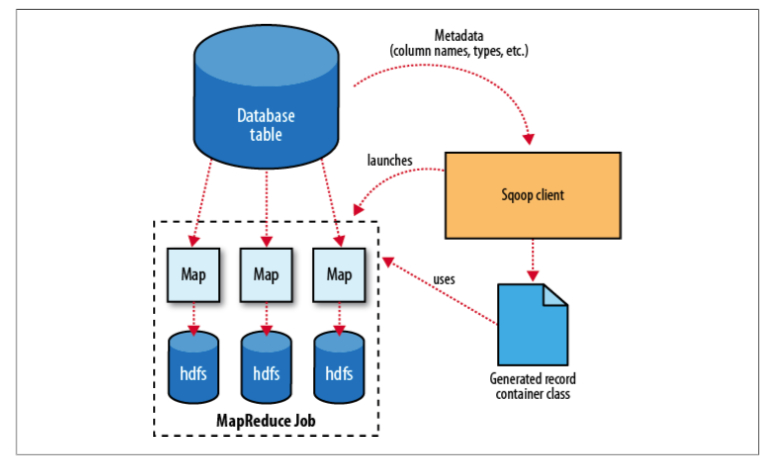
\includegraphics[scale=0.5]{Gambar/sqoop-import.png}
	\caption[Proses Impor Sqoop]{Proses Impor Sqoop} 
	\label{fig:sqoop_import}
\end{figure}

Gambar \ref{fig:sqoop_import} menggambarkan proses kerja impor pada Sqoop. Sqoop client akan membaca Metadata dari basisdata seperti \textit{field}, tipe data, dll melalui konektor JDBC. Kemudian Sqoop client secara otomatis akan membuat sebuah file java yang berisi kelas untuk melakukan proses impor menggunakan MapReduce. 

Berikut adalah contoh-contoh perintah pada Sqoop.

\begin{lstlisting}[caption=Perintah Impor Sqoop dari Basis Data MySQL ke HDFS]
	sqoop import --connect jdbc:mysql://localhost/nama_database \
	--username root  \
	--password your_password  \
	--table nama_tabel 
\end{lstlisting}

Pada kode di atas, Sqoop akan melakukan impor data dari basis data MySQL ke dalam HDFS.

\begin{lstlisting}[caption=Perintah Impor Sqoop dari Basis Data MySQL ke Hive]
	sqoop import --connect jdbc:mysql://localhost/nama_database \
	--table nama_tabel \ 
	--username root  \
	--password your_password \
	--hive-import \
	--fields-terminated-by ','  \
	--lines-terminated-by '\n'
\end{lstlisting}

Pada kode di atas, Sqoop akan melakukan impor data dari basis data MySQL ke dalam Hive dengan karakter koma sebagai pemisah antar \textit{field} dan baris baru sebagai pemisah antar \textit{record}.

\subsubsection{Ekspor Data Sqoop}
\label{sec:ekspor_data_sqoop}
Tool ekspor data Sqoop berfungsi untuk melakukan pemindahan data dari dalam HDFS ke luar HDFS. Cara kerja dari proses ekspor ini sangatlah mirip dengan proses impor yang sudah dibahas sebelumnya. 

(Lihat gambar \ref{fig:sqoop_ekspor}.) Sebelum melakukan ekspor, Sqoop client memulai dengan melakukan koneksi ke basis data menggunakan koneksi \textit{string} (kebanyakan sistem menggunakan JDBC). Kemudian Sqoop client akan membuat sebuah file kelas Java berdasarkan metadata pada tabel yang dituju. File yg dihasilkan dapat melakukan \textit{parsing} terhadap \textit{record-record} pada file teks di HDFS dan memasukan hasilnya ke dalam tabel. Setelah file kelas Java dibuat, maka sebuah MapReduce \textit{job} dimulai dan bertugas untuk membaca file di HDFS, \textit{parsing} data menggunakan kelas Java yang sudah dibuat, dan melakukan strategi expor data ke basisdata yang dituju.

\begin{figure}
	\centering
	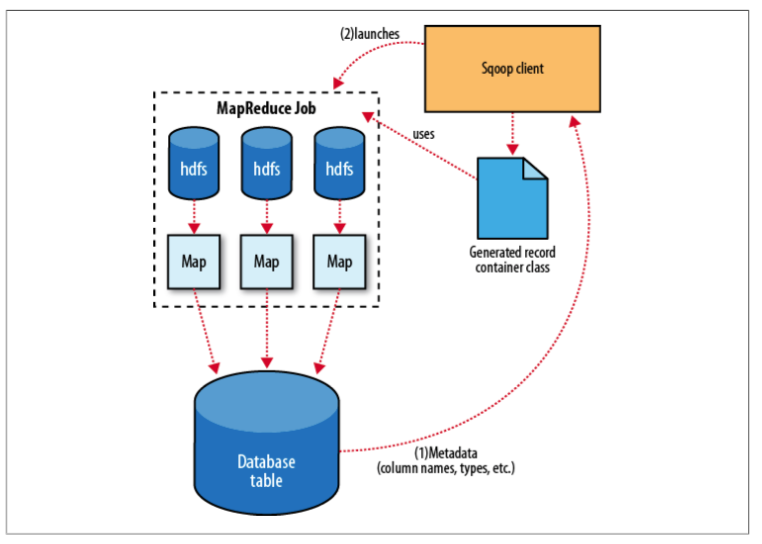
\includegraphics[scale=0.5]{Gambar/sqoop-export.png}
	\caption[Proses Ekspor Sqoop]{Proses Ekspor Sqoop} 
	\label{fig:sqoop_ekspor}
\end{figure}

\begin{lstlisting}[caption=Perintah Ekspor Sqoop dari HDFS ke Basis Data MySQL]
	sqoop export --connect jdbc:mysql://localhost/nama_database \
	--username root \
	--password your_password \
	--table nama_tabel  \
	--export-dir /path/to/your/data
\end{lstlisting}

Pada kode di atas, Sqoop akan melakukan ekspor data dari HDFS ke dalam basis data MySQL.

\begin{lstlisting}[caption=Perintah Ekspor Sqoop dari Hive ke Basis Data MySQL]
	sqoop import --connect jdbc:mysql://localhost/nama_database \
	--table nama_tabel \ 
	--username root \
	--password your_password \
	--export-dir /path/to/your/data \
	--fields-terminated-by ','  \
	--lines-terminated-by '\n'
\end{lstlisting}

Pada kode di atas, Sqoop akan melakukan ekspor data dari Hive ke dalam basis data MySQL dengan karakter koma sebagai pemisah antar \textit{field} dan baris baru sebagai pemisah antar \textit{record}.

\subsection{Apache Mahout}
\label{sec:apache_mahout}

\section{Algoritma Naive Bayes Classifier}
\label{sec:algoritma_naive_bayes}

\section{Algoritma SVN}
\label{sec:algoritma_svn}}{}
\ifdefstring{\vbabc}{1}{\chapter{Analisis dan Eksperimen}

\section{Analisis Masalah}
Keberadaan sosial media khususnya Twitter di Indonesia tidak dapat dipungkiri lagi sudah menjadi bagian hidup bagi kebanyakan orang. Masyarakat dapat menulis tentang apapun di sosial media miliknya, mulai dari opini pribadi tentang suatu barang atau jasa, membahas topik yang sedang hangat, ataupun hanya sekedar menuliskan lokasi keberadaannya saat ini. Namun sayangnya data yang tersebar di sosial media belum diolah dengan baik oleh para pemilik usaha. Padahal potensi yang dimiliki dari sosial media sangatlah besar bagi pertumbuhan usaha.

Salah satu sektor yang dapat memanfaatkan data dari sosial media adalah sektor pariwisata. Di sektor ini para pemilik usaha dapat memanfaatkan pesan dari sosial media untuk memprediksi tren wisata saat itu dan di masa depan. Selain itu mereka juga dapat mempelajari analisis sentimen negatif ataupun positif pengguna sosial media terhadap suatu lokasi wisata. 

Pesan media sosial saat ini khususnya Twitter jumlahnya sudah sangat banyak. Hal ini mengakibatkan pemilik usaha di bidang pariwisata kesulitan dalam mempelajari pesan-pesan tersebut secara manual. Masalah lainnya bagi mereka adalah pertumbungan pesan-pesan di sosial media yang berjalan dengan sangat cepat bahkan dalam hitungan detik datanya sudah berubah. 

Oleh karena itu, para pemilik usaha di bidang pariwisata memerlukan sebuah sistem yang dapat membantu mereka dalam mempelajari pesan-pesan di sosial media yang jumlahnya sangat banyak dan berkembang sangat cepat. Sistem yang dilengkapi dengan kecerdasan bisnis diharapkan dapat membantu para pemilik usaha di bidang pariwisata untuk melakukan pengambilan keputusan berdasarkan laporan, grafik dan hasil analisis sentimen dari pesan-pesan sosial media yang terkumpul di dalam \textit{datawarehouse}.

%\section{Analisis Data}

%\section{Analisis Sistem}

\section{Eksperimen}
Pada bagian ini, penulis melakukan uji coba beberapa kasus sederhana yang masih berhubungan dengan proses analisis text pada sosial media Twitter. Eksperimen yang dilakukan seperti membuat program Java untuk melakukan streaming data melalui Streaming API Twitter dan menyimpan hasilnya ke dalam file text. Selain itu penulis juga melakukan eksperimen untuk melakukan text preprocessing sederhana pada data tweet di lingkungan Hadoop.

\subsection{Streaming Tweet}
Dalam penelitian ini dibutuhkan tweet-tweet yang berhubungan dengan kegiatan pariwisata. Oleh karena itu penulis mencoba membuat sebuah program sederhana berbasis Java untuk melakukan streaming tweet. Kode sumber untuk eksperimen ini dapat dilihat pada Lampiran \ref{app:B}. Pada proses streaming tweet penulis menggunakan kata kunci  libur, liburan, travel, travelling, wisata, tour, pariwisata, destinasi, hotel, pesawat. Data tweet yang diambil juga dibatasi berdasarkan bahasa yang digunakan, hanya yang dalam bahasa Indonesia saja yang diambil. Berikut adalah salah satu contoh hasil tweet yang dihasilkan.

\begin{lstlisting}[language=Java,basicstyle=\tiny,caption=Hasil Streaming]
{
  "created_at": "Mon Sep 28 00:48:47 +0000 2015",
  "id": 6.4829827034363e+17,
  "id_str": "648298270343626752",
  "text": "Ujudkan ikon Pariwisata berwawasan lingkungan. Bali sdh banyak bermasalah dg air, fungsi lahan, dan sampah. http:\/\/t.co\/mj8l3D4xvy #AjegBali",
  "source": "<a href=\"http:\/\/twitter.com\/download\/iphone\" rel=\"nofollow\">Twitter for iPhone<\/a>",
  "truncated": false,
  "in_reply_to_status_id": null,
  "in_reply_to_status_id_str": null,
  "in_reply_to_user_id": null,
  "in_reply_to_user_id_str": null,
  "in_reply_to_screen_name": null,
  "user": {
    "id": 1690141351,
    "id_str": "1690141351",
    "name": "Bali Tolak Reklamasi",
    "screen_name": "ForBALI13",
    "location": "Bali",
    "url": "http:\/\/forbali.org",
    "description": "Official account Forum Rakyat Bali #TolakReklamasiTelukBenoa | Petisi: http:\/\/chn.ge\/1kyV5Bu | Ganti Profpic: http:\/\/twibbon.com\/support\/forbali-2",
    "protected": false,
    "verified": false,
    "followers_count": 43317,
    "friends_count": 178,
    "listed_count": 21,
    "favourites_count": 388,
    "statuses_count": 11135,
    "created_at": "Thu Aug 22 05:27:11 +0000 2013",
    "utc_offset": 21600,
    "time_zone": "Urumqi",
    "geo_enabled": false,
    "lang": "en",
    "contributors_enabled": false,
    "is_translator": false,
    "profile_background_color": "C0DEED",
    "profile_background_image_url": "http:\/\/pbs.twimg.com\/profile_background_images\/378800000077490261\/b733ff1364e61ccf11b48d972a419799.jpeg",
    "profile_background_image_url_https": "https:\/\/pbs.twimg.com\/profile_background_images\/378800000077490261\/b733ff1364e61ccf11b48d972a419799.jpeg",
    "profile_background_tile": true,
    "profile_link_color": "0084B4",
    "profile_sidebar_border_color": "FFFFFF",
    "profile_sidebar_fill_color": "DDEEF6",
    "profile_text_color": "333333",
    "profile_use_background_image": true,
    "profile_image_url": "http:\/\/pbs.twimg.com\/profile_images\/494053969430200320\/X2xjdPf-_normal.png",
    "profile_image_url_https": "https:\/\/pbs.twimg.com\/profile_images\/494053969430200320\/X2xjdPf-_normal.png",
    "profile_banner_url": "https:\/\/pbs.twimg.com\/profile_banners\/1690141351\/1402672316",
    "default_profile": false,
    "default_profile_image": false,
    "following": null,
    "follow_request_sent": null,
    "notifications": null
  },
  "geo": null,
  "coordinates": null,
  "place": null,
  "contributors": null,
  "retweet_count": 0,
  "favorite_count": 0,
  "entities": {
    "hashtags": [
      {
        "text": "AjegBali",
        "indices": [
          131,
          140
        ]
      }
    ],
    "trends": [
      
    ],
    "urls": [
      {
        "url": "http:\/\/t.co\/mj8l3D4xvy",
        "expanded_url": "http:\/\/bit.ly\/1PIgk0x",
        "display_url": "bit.ly\/1PIgk0x",
        "indices": [
          108,
          130
        ]
      }
    ],
    "user_mentions": [
      
    ],
    "symbols": [
      
    ]
  },
  "favorited": false,
  "retweeted": false,
  "possibly_sensitive": false,
  "filter_level": "low",
  "lang": "in",
  "timestamp_ms": "1443401327106"
}
\end{lstlisting}

Proses yang dilakukan pada eksperimen ini adalah
\begin{enumerate}
	\item Mendaftar di https://dev.twitter.com/ untuk mendapatkan \textit{consumer key,  consumer secret, access token,} dan \textit{access token secret} yang akan digunakan untuk mendapatkan data dari Twitter Streaming API.
	\item Membuat program Java dengan bantuan library org.scribe versi 1.3.7 yang berfungsi untuk melakukan autentikasi OAuth ke server Twitter.
	\item Mendapatkan tweet yang dikirim Twitter Streaming Server dan menyimpannya ke dalam file text.
\end{enumerate}
 
Dari hasil eksperimen ini ada beberapa hal yang perlu dievaluasi dan dikembangkan, yaitu:

\begin{itemize}
	\item Penulisan hasil streaming tweet langsung ke HDFS.
\end{itemize}


\subsection{Text Preprocessing Tweet Sederhana di Lingkungan Hadoop}
Untuk melakukan text mining pada tweet perlu diawali dengan text preprocessing terlebih dahulu. Oleh karena itu penulis melakukan eksperimen untuk melakukan text preprocessing sederhana pada data tweet di lingkungan sistem terdistribusi Hadoop. Kode sumber untuk eksperimen ini dapat dilihat pada Lampiran \ref{app:C}. Berikut adalah proses yang penulis lakukan pada eksperimen ini.

\begin{enumerate}
	\item Mengubah text ke dalam huruf kecil.
	\item Membuang stopwords pada tweet. Daftar stopwords yang digunakan dapat dilihat di Lampiran \ref{app:A}.
	\item Membuang tag ke pengguna lain (diawali dengan @) dan hashtag topik tertentu (diawali dengan \#).
	\item Membuang URL yang terdapat pada tweet.
	\item Menghilangkan karakter-karakter lainnya selain alfabet dari A sampai Z atau angka 0 sampai 9.
	\item Membuan spasi di awal dan akhir tweet serta menghilangkan multiple spasi.
\end{enumerate}
 
Untuk mendukung proses tersebut di atas dibutuhkan library pendukung lainnya yaitu org.apache.hadoop versi 2.7.1. Berikut adalah beberapa contoh masukan dan keluaran dari program sederhana ini.\\
 
     
\textbf{Masukan:}
\begin{enumerate}
	\item RT @CJRisCJR: Mau liburan ke Jepang bareng kita?Yuk ikut \#BoneetoTemuinKerenmu dari @BoneetoID ! Info, klik  http://t.co/THYLKLnSbX http://?
	\item @Hai @dimasarasta  Lets Joint With Us Wisata Seluler ke Jantungnya XL http://t.co/VPO4QyOBOt
	\item WISATA PULAU TIDUNG- Pemerintah Pusat Tetapkan Pantai Rupat jadi Tujuan Wisata Nasional - Metroterkini  http://t.co/LCUZJQveuX
	\item Paket Tour Karimunjawa 3hari 2malam | Mulai 805k/pax, min 8 pax | MoreInfo: 0271-733176, WA 089602910275, BB 5A4CC077 http://t.co/bc7os4f35J
	\item RT @detikcom: Ini Dampak Kabut Asap Terhadap Tour de Singkarak 2015 http://t.co/lNbnyPB485  via @detiktravel
\end{enumerate} 
     
\textbf{Keluaran:}
\begin{enumerate}
	\item liburan jepang bareng yuk info klik 
	\item lets joint with us wisata seluler jantungnya xl
	\item wisata pulau tidung pemerintah pusat tetapkan pantai rupat tujuan wisata nasional metroterkini
	\item paket tour karimunjawa 3hari 2malam 805kpax min 8 pax moreinfo 0271733176 wa 089602910275 bb 5a4cc077
	\item dampak kabut asap tour de singkarak 2015 via
\end{enumerate}

  
Dari hasil eksperimen ini ada beberapa hal yang perlu dievaluasi dan dikembangkan, yaitu:
\begin{itemize}
	\item Menghilangkan angka pada tweet, karena tidak dapat dimanfaatkan dalam proses text mining untuk mendapatkan sentimen tweetnya.
	\item Menambahkan daftar kata stopwords.
	\item Mengatasi penggunaan bahasa slang dan singkatan kata.
\end{itemize}
}{}
\ifdefstring{\vbabd}{1}{\chapter{Analisis Sistem Kecerdasan Bisnis}

\section{Analisis Data}
\subsection{Data Twitter}
Sumber data yang diambil dari Twitter menggunakan Twitter Streaming API akan menghasilkan data dalam format JavaScript Object Notation (JSON). Tabel \ref{tab:twitter_fields} adalah \textit{field-field} yang diambil untuk keperluan analisis pada penelitian ini. 

\begin{table}[!htb]
	\centering
	\begin{tabular}{| l | l | l |}
		\hline
		Field & Tipe & Deskripsi \\
	 	\hline
	 	id\_str & String & Unik \textit{identifier} untuk tweet dalam format string. \\
	 	text & String & Pesan twitter dengan encoding UTF-8. \\
	 	geo & Object & \textit{Nullable} Mendapatkan posisi pesan dibuat dalam bentuk\\
	 	& & latitude dan longitude. \\
	 	place & Places & \textit{Nullable}. Berisi data tempat yang berhubungan dengan\\
	 	& & tweet tapi tidak selalu asal lokasi tweet dibuat. \\
	 	timestamp\_ms & Timestamp & Berisi data waktu tweet dibuat dan ditampilkan dalam\\
	 	& & bentuk angka-angka (long).\\
	 	\hline
	\end{tabular}	
	\caption{Twitter Fields yang Digunakan}\label{tab:twitter_fields}
\end{table}	

\subsection{Data Instagram}
Sumber data lainnya yang digunakan untuk penelitian ini adalah data \textit{posting} dari Instagram yang biasanya disebut sebagai media. Instagram menyediakan banyak \textit{endpoint} yang dapat digunakan seperti users, relationships, media, comments, likes, tags dan locations. Untuk kasus pada penelitian ini penulis memilih \textit{endpoint} tags sebagai sumber data, karena data yang akan diambil adalah data dengan tags tertentu. Table \ref{tab:tag_endpoints} menjelaskan secara umum \textit{endpoint} apa saja yang terdapat di dalam kategori pencarian berdasarkan tag.

\begin{table}[H]
	\centering
	\begin{tabular}{| l | l | l |}
		\hline
		Method & URL & Deskripsi \\
		\hline
		GET & /tags/tag-name & Mendapatkan informasi tentang objek tag tersebut. \\
		GET & /tags/tag-name/media/recent & Mendapatkan sebuah \textit{list} media dengan tag tertentu. \\
		GET & /tags/search & Mencari variasi tag dengan keyword tertentu.\\
		\hline
	\end{tabular}	
	\caption{Tag Endpoints}\label{tab:tag_endpoints}
\end{table}	

Di antara tag \textit{endpoints} yang ada, yang paling relevan dengan kebutuhan analisis adalah tag \textit{endpoint} dengan kembalian \textit{list} media karena data dari medialah yang akan dianalisis. Untuk menggunakan \textit{endpoint} tersebut ada beberapa parameter yang harus diperhatikan (lihat Table \ref{tab:tag_endpoints_media}).

\begin{table}[H]
	\centering
	\begin{tabular}{| l | l |}
		\hline
		Parameter & Deskripsi \\
		\hline
		ACCESS\_TOKEN & Sebuah access token yang valid. \\
		COUNT & Jumlah media yang akan dikembalikan. \\
		MIN\_TAG\_ID & Mengembalikan media sebelum min\_tag\_id tertentu. \\
		MAX\_TAG\_ID & Mengembalikan media sesudah max\_tag\_id tertentu. \\
		\hline
	\end{tabular}	
	\caption{Tag Endpoint Media Recent}\label{tab:tag_endpoints_media}
\end{table}	

\textit{Endpoint} tersebut akan menghasilkan kembalian dalam format json berupa \textit{list} media-media. Setiap data media memiliki attribut-attribut yang dikembalikan seperti caption, image, dll (lihat Listing \ref{lst:response_tag_endpoint_media}). Pada penelitian ini data yang akan diteliti berdasarkan caption yang dibuat dan juga lokasi. Oleh karena itu data-data yang akan diambil pada penelitian ini hanyalah data pada atribut-atribut di tabel \ref{tab:instagram_fields}. 

Selain mengembalikan data-data media, \textit{endpoint} ini juga mengembalikan attribut \textit{pagination} yang berisi \textit{next\_url} dan data-data \textit{pagination} lainnya. Data tersebut digunakan untuk melakukan \textit{request} ke halaman berikutnya, informasi lebih detail tentang ini akan dibahas pada Bab \ref{sec:dfd_streaming_instagram}.

\begin{table}[H]
	\centering
	\begin{tabular}{| l | l | l |}
		\hline
		Field & Tipe & Deskripsi \\
	 	\hline
	 	id & String & Unik \textit{identifier} untuk media dalam format string. \\
	 	caption.text & String & Caption untuk media. \\
	 	location.name & String &  \textit{Nullable}. Berisi keterangan lokasi yang dimasukan oleh \\
	 	& & pengguna ketika mengunggah. \\
	 	created\_time & Timestamp & Berisi data waktu media dibuat dan ditampilkan dalam \\
	 	& & bentuk angka-angka (long).\\
		\hline
	\end{tabular}	
	\caption{Instagram Fields yang digunakan}\label{tab:instagram_fields}
\end{table}	

\begin{lstlisting}[basicstyle=\tiny,caption=Response Tag Endpoint Media Recent,label={lst:response_tag_endpoint_media}]
	{
	"pagination": {
		"next_url": "...",
		"prev_url": "...",
		...
	},
    "data": [{
        "type": "image",
        "users_in_photo": [],
        "filter": "Earlybird",
        "tags": ["snow"],
        "comments": {
            "count": 3
        },
        "caption": {
            "created_time": "1296703540",
            "text": "#Snow",
            "from": {
                "username": "emohatch",
                "id": "1242695"
            },
            "id": "26589964"
        },
        "likes": {
            "count": 1
        },
        "link": "http://instagr.am/p/BWl6P/",
        "user": {
            "username": "emohatch",
            "profile_picture": "http://distillery.s3.amazonaws.com/profiles/profile_1242695_75sq_1293915800.jpg",
            "id": "1242695",
            "full_name": "Dave"
        },
        "created_time": "1296703536",
        "images": {
            "low_resolution": {
                "url": "http://distillery.s3.amazonaws.com/media/2011/02/02/f9443f3443484c40b4792fa7c76214d5_6.jpg",
                "width": 306,
                "height": 306
            },
            "thumbnail": {
                "url": "http://distillery.s3.amazonaws.com/media/2011/02/02/f9443f3443484c40b4792fa7c76214d5_5.jpg",
                "width": 150,
                "height": 150
            },
            "standard_resolution": {
                "url": "http://distillery.s3.amazonaws.com/media/2011/02/02/f9443f3443484c40b4792fa7c76214d5_7.jpg",
                "width": 612,
                "height": 612
            }
        },
        "id": "22699663",
        "location": null
    },
    {
        "type": "video",
        "videos": {
            "low_resolution": {
                "url": "http://distilleryvesper9-13.ak.instagram.com/090d06dad9cd11e2aa0912313817975d_102.mp4",
                "width": 480,
                "height": 480
            },
            "standard_resolution": {
                "url": "http://distilleryvesper9-13.ak.instagram.com/090d06dad9cd11e2aa0912313817975d_101.mp4",
                "width": 640,
                "height": 640
            },
        "users_in_photo": null,
        "filter": "Vesper",
        "tags": ["snow"],
        "comments": {
            "count": 2
        },
        "caption": {
            "created_time": "1296703540",
            "text": "#Snow",
            "from": {
                "username": "emohatch",
                "id": "1242695"
            },
            "id": "26589964"
        },
        "likes": {
            "count": 1
        },
        "link": "http://instagr.am/p/D/",
        "user": {
            "username": "kevin",
            "full_name": "Kevin S",
            "profile_picture": "...",
            "id": "3"
        },
        "created_time": "1279340983",
        "images": {
            "low_resolution": {
                "url": "http://distilleryimage2.ak.instagram.com/11f75f1cd9cc11e2a0fd22000aa8039a_6.jpg",
                "width": 306,
                "height": 306
            },
            "thumbnail": {
                "url": "http://distilleryimage2.ak.instagram.com/11f75f1cd9cc11e2a0fd22000aa8039a_5.jpg",
                "width": 150,
                "height": 150
            },
            "standard_resolution": {
                "url": "http://distilleryimage2.ak.instagram.com/11f75f1cd9cc11e2a0fd22000aa8039a_7.jpg",
                "width": 612,
                "height": 612
            }
        },
        "id": "3",
        "location": null
    },
    ...]
}
\end{lstlisting}

\section{Analisis Masalah}
\label{sec:analisis_masalah}
Keberadaan sosial media khususnya Twitter dan Instagram di Indonesia sudah menjadi bagian hidup bagi kebanyakan orang. Masyarakat dapat menulis tentang apapun di sosial media miliknya. Namun sayangnya data yang tersebar di sosial media belum diolah dengan baik oleh para pemilik usaha. Padahal potensi yang dimiliki dari sosial media sangatlah besar bagi pertumbuhan usaha.

Salah satu sektor yang dapat memanfaatkan data dari sosial media adalah sektor pariwisata. Di sektor ini para pemilik usaha (\textit{travel agent}) dapat memanfaatkan pesan dari sosial media untuk mendapatkan informasi tren wisata saat itu. Selain para pemilik usaha, masih terdapat pihak-pihak lain yang dapat memanfaatkan pesan dari sosial media, seperti pemerintah melalui dinas pariwisata, wisatawan / \textit{backpacker} dan maskapai penerbangan atau penyedia layanan transportasi. 

Pesan media sosial saat ini khususnya Twitter dan Instagram jumlahnya sudah sangat banyak. Hal ini mengakibatkan pemilik usaha di bidang pariwisata kesulitan dalam menganalisis tren wisata yang sedang terjadi secara manual. Masalah lainnya bagi mereka adalah pertumbungan pesan-pesan di sosial media yang berjalan dengan sangat cepat bahkan dalam hitungan detik datanya sudah berubah. 

Oleh karena itu, para pemilik usaha di bidang pariwisata memerlukan sebuah sistem yang dapat membantu mereka dalam menganalisis tren wisata di sosial media yang jumlahnya sangat banyak dan berkembang sangat cepat. Sistem yang dilengkapi dengan kecerdasan bisnis diharapkan dapat membantu para pemilik usaha di bidang pariwisata untuk melakukan pengambilan keputusan berdasarkan laporan, grafik dan hasil analisis dari pesan-pesan sosial media yang terkumpul di dalam \textit{data warehouse}. Contoh pengetahuan-pengetahuan yang dapat dihasilkan dari sistem kecerdasan bisnis ini antara lain:

\begin{itemize}
	\item Mengetahui waktu-waktu ramai suatu lokasi wisata dikunjungi wisatawan. Dengan adanya informasi ini pemilik usaha dapat lebih mudah dalam melakukan promosi serta mempersiapkan pelayanan yang lebih baik untuk pelanggan ketika waktu-waktu ramai dan mengurangi pengeluaran-pengeluaran ketika waktu-waktu sepi. 
	\item Mengukur potensi wisata suatu daerah. Dengan adanya informasi ini pemerintah dapat melihat potensi-potensi wisata yang dimiliki suatu daerah, sehingga mempermudah dalam menentukan prioritas pembangunan di suatu lokasi wisata yang cukup favorit untuk dikunjungi.
	\item Mempersiapkan infrastruktur dan fasilitas yg memadai di saat-saat ramai. Dengan adanya informasi ini instansi pemerintah terkait juga dapat mempersiapkan dengen lebih matang infrastruktur, fasilitas, serta pengamanan di lokasi maupun akses menuju lokasi untuk kepuasan dan keselamatan para wisatawan selama berwisata. 
\end{itemize}
}{}
\ifdefstring{\vbabe}{1}{\chapter{Implementasi, Pengujian dan Eksperimen}
\section{Deskripsi Perangkat Keras dan Lunak yang Digunakan}
\label{sec:deskripsi_perangkat_keras}
Pada penelitian ini terdapat dua tahap implementasi. Implementasi pertama dilakukan di komputer peneliti untuk keperluan pengujian fungsional. Komputer tersebut memiliki spesifikasi sebagai berikut:

\begin{enumerate}
	\item Processor: 2.5 GHz Intel Core i5
	\item RAM: 10 GB DDR3
	\item Sistem Operasi: OS X El Capitan (v10.11.3)
	\item Versi Java: 1.8.0\_45
	\item Apache Hadoop: 2.7.1
	\item Apache Hive: 1.2.1
	\item Apache Sqoop: 1.4.6
	\item MySQL: 5.5.40
	\item Pentaho Data Integration (PDI): Community Edition 6.0.1.0
\end{enumerate}

Implementasi kedua dilakukan pada komputer laboratorium untuk pengujian eksperimental. Jumlah total komputer yang digunakan untuk eksperimen adalah 1 buah komputer \textit{master} dan 25 komputer \textit{slave}. Komputer-komputer tersebut memiliki spesifikasi sebagai berikut:
\begin{enumerate}
	\item Processor: 3.3 GHz Intel Core i3
	\item RAM: 4 GB DDR3
	\item Sistem Operasi: Ubuntu 14.04 LTS
	\item Versi Java: 1.8.0\_45
	\item Apache Hadoop: 2.7.1
	\item Apache Hive: 1.2.1
	\item Apache Sqoop: 1.4.6
	\item MySQL: 5.5.40
	\item Pentaho Data Integration (PDI): Community Edition 6.0.1.0
\end{enumerate}

\section{Implementasi Modul Program}
\subsection{Implementasi Modul Program \textit{Streaming} Twitter}
Implementasi modul program \textit{streaming} Twitter akan terbagi menjadi dua buah bagian yaitu implementasi antarmuka program dan implementasi kode di dalamnya. 

\subsubsection{Implementasi Antar Muka \textit{Streaming} Twitter}
Gambar \ref{fig:ui_implementasi_streaming_twitter} merupakan hasil implementasi dari modul program ini. Implementasi antarmuka modul program ini dibuat menggunakan Java Swing. 

Pengguna dapat memasukan data-data seperti consumer key, consumer secret, access token dan access token secret sesuai dengan data yang didapatkan dari Twitter Streaming API. Selain itu pengguna juga dapat memasukan kata kunci untuk mendapatkan \textit{tweet} yang relevan dengan kebutuhan organisasi. Untuk pilihan lokasi penyimpanan, pengguna dapat menggunakan \textit{radio button} dan mengisi lokasi \textit{path}.
 
\begin{figure}[H]
	\centering
	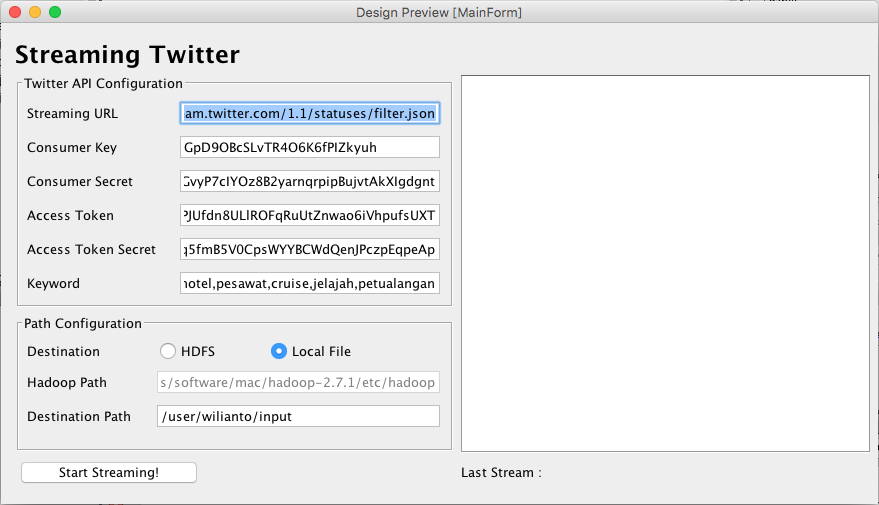
\includegraphics[scale=0.5]{Gambar/ui-implementasi-streaming-twitter.png}
	\caption[Implementasi Antarmuka \textit{Streaming} Twitterr]{Implementasi Antarmuka \textit{Streaming} Twitter} 
	\label{fig:ui_implementasi_streaming_twitter}
\end{figure}


\subsubsection{Implementasi Kode Program \textit{Streaming} Twitter}
Kode program pada modul ini ditulis menggunakan program Java. Berikut adalah potongan-potongan kode hasil implementasi dari modul progam ini. 

\begin{lstlisting}[language=Java,basicstyle=\tiny,caption=Writer.java,label={lst:kode_writer}]
public interface Writer {
    public void write(String path, String content);
    public void close();
}
\end{lstlisting}

\begin{lstlisting}[language=Java,basicstyle=\tiny,caption=LocalOperation.java,label={lst:kode_local_operation}]
public class LocalOperation implements Writer{
    protected String fileName;
    protected FileWriter fw;

    @Override
    public void write(String path, String content) {
        try {
            if(this.fw == null){
                this.fw = new FileWriter(path);
            }
            
            fw.append(content);
        } catch (IOException ex) {
            System.out.println(ex.toString());
        }
    }
    
    ....
}
\end{lstlisting}

\begin{lstlisting}[language=Java,basicstyle=\tiny,caption=HDFSOperation.java,label={lst:kode_hdfs_operation}]
public class HDFSOperation implements Writer{
    protected String hadoopPath;
    protected Configuration conf;
    protected FileSystem fs;
    
    protected void init(){
        conf = new Configuration();
        conf.addResource(new Path(hadoopPath + "/core-site.xml"));
        conf.addResource(new Path(hadoopPath + "/hdfs-site.xml"));
        conf.set("fs.hdfs.impl", org.apache.hadoop.hdfs.DistributedFileSystem.class.getName());
        conf.set("fs.file.impl", org.apache.hadoop.fs.LocalFileSystem.class.getName());
        try {
            fs = FileSystem.get(conf);
        } catch (IOException ex) {
            System.out.println(ex.getMessage());
        }
    }
    
    public void write(String hdfsPath, String content) {
        Path path = new Path(hdfsPath);
        try{
            FSDataOutputStream fos;
            //delete file if exist
            if(fs.exists(path)){
                fos = fs.append(path);
            }else{
                fos = fs.create(path);
            }
            
            //create file and write content to file
            fos.writeUTF(content);
            fos.close();
        }catch(IOException ex){
            System.out.println(ex.getMessage());
        }
    }
    
    public String read(String hdfsPath) {
        String content = null;
        Path path = new Path(hdfsPath);
        try{
            //create file and write content to file
            FSDataInputStream fis = fs.open(path);
            BufferedReader reader = new BufferedReader(new InputStreamReader(fis.getWrappedStream()));
            String s;
            while((s = reader.readLine()) != null){
                content += s;
            }
            reader.close();
            fis.close();
        }catch(IOException ex){
            System.out.println(ex.getMessage());
        }
        return content;
    }
    
    public void copyFromLocal(String localPath, String hdfsPath){
        Path srcPath = new Path(localPath);
        Path destPath = new Path(hdfsPath);
        
        try{
            //check is path exist
            if(fs.exists(destPath)){
                System.out.println("No such destination " + destPath);
                return;
            }
            
            fs.copyFromLocalFile(srcPath, destPath);
        }catch(IOException ex){
            System.out.println(ex.getMessage());
        }
    }
    
    public void delete(String hdfsPath) {
        Path path = new Path(hdfsPath);
        try{
            fs.delete(path, true);
        }catch(IOException ex){
            System.out.println(ex.getMessage());
        }
    }
    
    ....
}
\end{lstlisting}

\begin{lstlisting}[language=Java,basicstyle=\tiny,caption=TwitterStreamer.java,label={lst:kode_twitter_streamer}]

public class TwitterStreamer extends Thread {

    ....
    
    public TwitterStreamer(String streamUrl, String consumerKey, String consumerSecret, String accessToken, String accessTokenSecret, String keyword, String hadoopPath, String filePath, JTextArea textArea, JLabel lastStreamLabel) {
        
        ....
        
        if(this.hadoopPath != ""){
            this.writer = new HDFSOperation(hadoopPath);
        }else{
            this.writer = new LocalOperation();
        }
    }

    public void run() {
        try {
            OAuthService service = new ServiceBuilder()
                    .provider(TwitterApi.class)
                    .apiKey(consumerKey)
                    .apiSecret(consumerSecret)
                    .build();

            //set access token
            textArea.setText("Started...\n");
            Token accessTokenGenerated = new Token(accessToken, accessTokenSecret);

            //generate the request
            OAuthRequest request = new OAuthRequest(Verb.POST, streamUrl);
            request.addHeader("version", "HTTP/1.1");
            request.addHeader("host", "stream.twitter.com");
            request.setConnectionKeepAlive(true);
            request.addHeader("user-agent", "Twitter Stream Reader");
            request.addBodyParameter("track", keyword); 
            request.addBodyParameter("language", "in");
            service.signRequest(accessTokenGenerated, request);
            Response response = request.send();
            
            BufferedReader reader = new BufferedReader(new InputStreamReader(response.getStream()));
            
            String line;
            JSONObject jsonObj;
            String sourceId, text, geo, place, timestampMs, appendLine;
            SimpleDateFormat sdf = new SimpleDateFormat("MMM dd,yyyy HH:mm:ss");    
            Date date;
            while ((line = reader.readLine()) != null && start) {
                try{
                    jsonObj = new JSONObject(line);
                    if(jsonObj.has("text") && jsonObj.get("text") != null){
                        sourceId = jsonObj.has("id_str") ? jsonObj.getString("id_str") : null;
                        text = jsonObj.has("text") ? jsonObj.getString("text") : null;
                        geo = jsonObj.has("geo") ? jsonObj.get("geo").toString() : null;
                        place = jsonObj.has("place") ? jsonObj.get("place").toString() : null;
                        timestampMs = jsonObj.has("timestamp_ms") ? jsonObj.getString("timestamp_ms") : null;
                        appendLine = sourceId + "\t" + text.replaceAll("\\n", " ") + "\t" + geo + "\t" + place + "\t" + timestampMs + "\t";
                        textArea.setText(counter + " data.");
                        writer.write(filePath, appendLine + "\n");
                        date = new Date(System.currentTimeMillis());
                        lastStreamLabel.setText(sdf.format(date));
                        counter++;
                    }
                }catch(Exception e){
                }
            }
            writer.close();
            textArea.setText(textArea.getText() + "Stopped...\n");
        } catch (IOException ex) {
            ex.printStackTrace();
        }
    }
    
    ....
}
\end{lstlisting}

\subsection{Implementasi Modul Program \textit{Crawling} Instagram}
Implementasi modul program \textit{crawling} Instagram akan terbagi menjadi dua buah bagian yaitu implementasi antarmuka program dan implementasi kode di dalamnya. 

\subsubsection{Implementasi Antar Muka \textit{Crawling} Instagram}
Gambar \ref{fig:ui_implementasi_streaming_instagram} merupakan hasil implementasi dari modul program ini. Implementasi antarmuka modul program ini dibuat menggunakan Java Swing. 

Pengguna dapat memasukan data-data seperti \textit{client ID, client secret} dan \textit{redirect URL} sesuai dengan data yang didapatkan dari Instagram API. Selain itu pengguna juga dapat memasukan tag untuk mendapatkan media dengan caption yang relevan dengan kebutuhan organisasi. Untuk pilihan lokasi penyimpanan, pengguna dapat menggunakan \textit{radio button} dan mengisi lokasi \textit{path}. Namun sebelum memulai pengguna harus mendapatkan \textit{code} terlebih dahulu dengan cara mengklik tombol "Get Code", lalu login dengan akun Instagramnya di browser. Setelah berhasil pengguna akan diarahkan ke sebuah halaman yang berisi \textit{code}.

\begin{figure}[H]
	\centering
	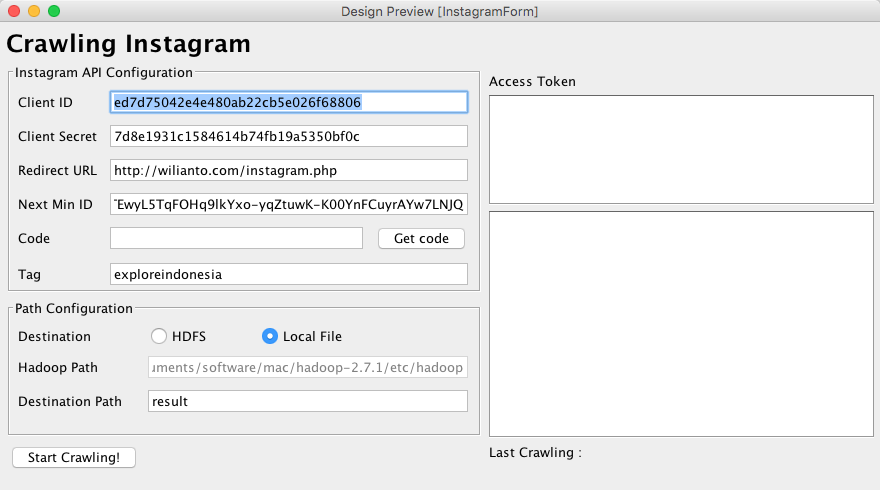
\includegraphics[scale=0.5]{Gambar/ui-implementasi-crawling-instagram.png}
	\caption[Implementasi Antarmuka \textit{Crawling} Instagram]{Implementasi Antarmuka \textit{Crawling} Instagram} 
	\label{fig:ui_implementasi_streaming_instagram}
\end{figure}

\subsubsection{Implementasi Kode Program \textit{Crawling} Instagram}
Kode program pada modul ini ditulis menggunakan program Java. Untuk kode Writer.java, HDFSOperation.java dan LocalOperation.java dapat dilihat pada Listing \ref{lst:kode_writer}, \ref{lst:kode_hdfs_operation} dan \ref{lst:kode_local_operation}. Berikut adalah kode-kode hasil implementasi dari modul progam ini. 

\begin{lstlisting}[language=Java,basicstyle=\tiny,caption=TwitterStreamer.java,label={lst:kode_instagram_crawler}]
public class InstagramCrawler extends Thread{
    ....
    
    public InstagramCrawler(String clientId, String clientSecret, String redirectUrl, String code, String nextMinId, String tag, String hadoopPath, String filePath, JTextArea textArea, JLabel lastStreamLabel, JTextField minTagIdTextField, JTextArea jsonTextArea, JButton triggerBtn, InstagramForm form) {
        ....
        
        if(this.hadoopPath != ""){
            this.writer = new HDFSOperation(hadoopPath);
        }else{
            this.writer = new LocalOperation();
        }
    }
    
    @Override
    public void run() {
        try {
            this.getAccessToken();
            writer.close();
            logWriter.close();
        } catch (IOException ex) {
            Logger.getLogger(InstagramCrawler.class.getName()).log(Level.SEVERE, null, ex);
        }
    }
    
    protected String generateUrl(){
        String url = "https://api.instagram.com/v1/tags/" + tag + "/media/recent"
                + "?count=100"
                + "&min_tag_id=" + nextMinId
                + "&access_token=" + accessToken;
        return url;
    }
    
    public void getAccessToken() throws MalformedURLException, IOException{
        this.start = true;
        triggerBtn.setText("Stop Crawling!");
        textArea.setText("Started...\n");
        
        if(this.accessToken == null || this.accessToken.isEmpty()){
            textArea.setText("Requesting access token...\n");

            //set URL
            url = new URL("https://api.instagram.com/oauth/access_token");

            //create connection with GET method
            conn = (HttpURLConnection) url.openConnection();
            conn.setRequestMethod("POST");
            //create data in URL format
            String data = "client_id=" + clientId
                    + "&client_secret=" + clientSecret
                    + "&grant_type=authorization_code"
                    + "&redirect_uri=" + redirectUrl
                    + "&code=" + code;

            //get output stream from connection to send the data
            conn.setDoOutput(true);
            OutputStream os = new BufferedOutputStream(conn.getOutputStream());
            os.write(data.getBytes());
            os.flush();
            os.close();

            //read the returned data
            br = new BufferedReader(new InputStreamReader(conn.getInputStream()));

            result = "";
            while((line = br.readLine()) != null){
                result += line;
            }
            json = new JSONObject(result);
            if(json.has("access_token")){
                this.accessToken = json.getString("access_token");
                jsonTextArea.setText(this.accessToken); 
                
                textArea.setText("Access token created...\n");
                this.getTagMediaRecent(this.generateUrl());
            }else{
                this.start = false;
                triggerBtn.setText("Start Crawling!");
                return;
            }
        }else{
            textArea.setText("Access token created...\n");
            this.getTagMediaRecent(this.generateUrl());
        }
    }
    
    public void getTagMediaRecent(String urlTagMediaRecent) 
            throws MalformedURLException, IOException {
        //set URL
        url = new URL(urlTagMediaRecent);

        //create connection with GET method
        conn = (HttpURLConnection) url.openConnection();
        conn.setRequestMethod("GET");

        //read the returned data
        br = new BufferedReader(new InputStreamReader(conn.getInputStream()));

        result = "";
        while((line = br.readLine()) != null){
            result += line;
        }

        //parse json object
        json = new JSONObject(result);
        datas = json.getJSONArray("data");

        for(int i = 0; i < datas.length(); i++){
            data = datas.getJSONObject(i);

            try{
                caption = (data.get("caption") != null) ? data.getJSONObject("caption") : null;
                location = (data.get("location") != null) ? data.get("location").toString() : null;
                locationName = (location != null) ? data.getJSONObject("location").getString("name") : "";
                text = caption != null ? caption.getString("text") : " ";
                text = text.replaceAll("\\n", " ");
                text = text + " " + locationName;
                //standard format with twitter streamer
                appendLine = "instagram-" + data.getString("id") + "\t" + text + "\t instagram \t" + location + "\t" + data.getString("created_time") + "000\t";
                textArea.setText(counter + " data.");
                writer.write(filePath, appendLine + "\n");
                date = new Date(System.currentTimeMillis());
                lastStreamLabel.setText(sdf.format(date));
                counter++;
            }catch(Exception ex){
            }
        }
        br.close();

        //do recursively
        pagination = json.getJSONObject("pagination");
        nextMinId = pagination.getString("next_min_id");
        nextUrl = pagination.has("next_url") ? pagination.getString("next_url") : null;
        logWriter.write("log.txt", sdf.format(date) + "\t" + tag + "\t" + nextMinId + "\n");

        if(nextUrl != null && start && counter < 15000){ 
            depth++;
            minTagIdTextField.setText(nextMinId);
            getTagMediaRecent(nextUrl);
        }else{
            minTagIdTextField.setText(nextMinId);
            textArea.setText(textArea.getText() + "\nStopped...");
            this.stopCrawling();
            //if not terminated by user, run new thread again
            if(!this.terminatedByUser){
                this.form.run();
            }
        }
    }
    
    ....
}
\end{lstlisting}

\subsection{Implementasi Modul Program Pembersihan Data dan Penghitungan Frekuensi Lokasi Wisata}
Implementasi pada modul ini dibuat menjadi dua buah program. Program utama menggunakan MapReduce sedangkan program kedua tanpa MapReduce. Tujuannya untuk mendapatkan hasil pengujian kedua buah program dari sisi waktu eksekusi. 

Potongan kode program pada Listing \ref{lst:kode_trie_node}, \ref{lst:kode_trie} dan \ref{lst:kode_cleaner} digunakan oleh kedua buah program. Listing \ref{lst:kode_trie_node} dan \ref{lst:kode_trie} merupakan kelas-kelas yang mengimplementasikan struktur data Trie yang sederhana untuk keperluan penyimpanan (\textit{dictionary}) kata lokasi wisata. Listing \ref{lst:kode_cleaner} merupakan implementasi kelas yang digunakan untuk melakukan pembersihan pada data sebelum diproses lebih lanjut.

Listing \ref{lst:kode_mapreduce} adalah potongan kode program yang menggunakan MapReduce. Pada kelas Map, dilakukan pembersihan data kemudian pencarian lokasi wisata yang terkandung di dalam data. Sedangkan pada kelas Reduce, dilakukan pengumpulan kata-kata hasil pencarian di Map dan dilakukan penghitungan frekuensi kemunculan kata di dalam suatu waktu.

Listing \ref{lst:kode_tanpa_mapreduce} adalah potongan kode program yang tidak menggunakan MapReduce. Tahapan yang dilakukan sama dengan program MapReduce, namun program hanya dapat dijalankan pada komputer tunggal saja.

\begin{lstlisting}[language=Java,basicstyle=\tiny,caption=TrieNode.java,label={lst:kode_trie_node}]
public class TrieNode {
    ....

    public TrieNode(){
        this.children = new TrieNode[38]; //26char, 10number, 1 space, 1 stripe
    }
    
    ....

    public void addNode(char c){
        int i = -1;
        if((int) c >= 48 && (int) c <= 57){
            //0-9
            i = (int) c - 48;
        }else if((int) c == 32){
            //space
            i = 10;
        }else if((int) c >= 97 && (int) c <= 122){
            //a-z
            i = (int) c - 97 + 11;
        }else if((int) c == (int) '-'){
            //strip
            i = 37;
        }
        if(i >= 0 && this.children[i] == null){
            this.children[i] = new TrieNode();
        }
    }
    
    public TrieNode getNode(char c){
        int i = -1;
        if((int) c >= 48 && (int) c <= 57){
            //0-9
            i = (int) c - 48;
        }else if((int) c == 32){
            //space
            i = 10;
        }else if((int) c >= 97 && (int) c <= 122){
            //a-z
            i = (int) c - 97 + 11;
        }else if((int) c == (int) '-'){
            //strip
            i = 37;
        }
        return (i >= 0) ? this.children[i] : null;
    }
}
\end{lstlisting}

\begin{lstlisting}[language=Java,basicstyle=\tiny,caption=Trie.java,label={lst:kode_trie}]
public class Trie {
	....
	
    public Trie(){
        this.root = new TrieNode();
    }
    
    ....
    
    public void addWord(String word){
        word = word.toLowerCase();
        char[] cs = word.toCharArray();
        TrieNode node = this.root;
        for (int i = 0; i < cs.length; i++) {
            node.addNode(cs[i]);
            node = node.getNode(cs[i]);
        }
        node.setWord(true);
    }

    public String findWord(String word){
        String s = "";
        char[] cs = word.toCharArray();
        TrieNode node = this.root;
        for (int i = 0; i < cs.length; i++) {
            if(node.getNode(cs[i]) != null){
                s += cs[i];
                node = node.getNode(cs[i]);
            }else{
                return null;
            }
        }
        return node.isWord() ? s : (node.getNode(' ') != null ? "%" : null);
    }
    
}
\end{lstlisting}

\begin{lstlisting}[language=Java,basicstyle=\tiny,caption=Cleaner.java,label={lst:kode_cleaner}]
public class Cleaner {
	....
	    
    private String replaceMap(String line){
        String[] words = line.split(" ");
        String newLine = "";
        
        for(String word : words){
            newLine += (replaceMap.containsKey(word) ? replaceMap.get(word).toLowerCase() : word) + " ";
        }
        
        return newLine;
    }
    
    private String removeStopword(String line){
        //replace user tag
        line = line.replaceAll("(@|#)(\\w+)", "");
        //replace http URL
        line = line.replaceAll("(https|http)://[\\w\\d\\.\\/\\?\\-\\+%=&#]+", "");
        //replace selain alfabet, numberik atau spasi
        line = line.replaceAll("[^A-Za-z0-9 ]", "");
        //trim first and last space character
        line = line.trim();
        //remote multiple spaces in sentence
        line = line.replaceAll(" +", " ");
        return line;
    }
}
\end{lstlisting}

\begin{lstlisting}[language=Java,basicstyle=\tiny,caption=Counter.java (MapReduce),label={lst:kode_mapreduce}]
public class Counter {
	....
    public static class WordMapper extends Mapper<Object, Text, Text, IntWritable>{
        ....
        @Override
        public void map(Object obj, Text text, Context context) 
                throws IOException, InterruptedException{
            String line = text.toString().toLowerCase();
            String[] parse = line.split("\t");
            String value = "";
            
            if(parse.length >= 2){
                value = cleaner.clean(parse[1]); 
            }
            
            SimpleDateFormat df = new SimpleDateFormat("YYYY-MM-dd");
            String term = "";
            String result;
            String[] sentences = value.split(" ");
            for(String sentence : sentences){
                if(term.isEmpty()){
                    result = destinationTrie.findWord(sentence);
                    if(parse.length >= 5){
                        if(result != null){
                            if(result.equals("%")){
                                term = sentence + " ";
                            }else{
                                context.write(new Text(result + "\t" + df.format(new Date(Long.parseLong(parse[parse.length - 1])))), new IntWritable(1));
                            }
                        }
                    }
                }else{
                    result = destinationTrie.findWord(term + sentence);
                    if(parse.length >= 5){
                        if(result != null){
                            if(result.equals("%")){
                                term += sentence + " ";
                            }else{
                                context.write(new Text(result + "\t" + df.format(new Date(Long.parseLong(parse[parse.length - 1])))), new IntWritable(1));
                            }
                        }else{
                            //reset term
                            term = "";
                        } 
                    }
                }
            }
        }
    }
    
    public static class DateReducer extends Reducer<Text, IntWritable, Text, IntWritable>{        
        @Override
        public void reduce(Text key, Iterable<IntWritable> values, Context context) 
                throws IOException, InterruptedException{
            int i = 0;
            for(IntWritable value : values){
                i += value.get();
            }            
            context.write(key, new IntWritable(i));
        }
    }
}
\end{lstlisting}

\begin{lstlisting}[language=Java,basicstyle=\tiny,caption=Counter.java (Tanpa MapReduce),label={lst:kode_tanpa_mapreduce}]
public class Counter {
	....
	public void count() throws IOException{
        //read all file at input folder
        File folder = new File(inputFolder);
        File[] files = folder.listFiles();
        String line, result, term, msg, date, key;
        String[] parse, sentences;
        SimpleDateFormat df = new SimpleDateFormat("YYYY-MM-dd");
        
        for(File file : files){
            System.out.println("Reading file " + file.getName());
            fr = new FileReader(file);
            br = new BufferedReader(fr);
            
            while((line = br.readLine()) != null){
                parse = line.split("\t");
                if(parse.length >= 5){
                    term = "";
                    msg = this.cleaner.clean(parse[1].toLowerCase());
                    sentences = msg.split(" ");
                    for(String word : sentences){
                        if(term.isEmpty()){
                            result = trie.findWord(word);
                            if(result != null){
                                if(result.equals("%")){
                                    term = word + " ";
                                }else{
                                    try{
                                        date = df.format(new Date(Long.parseLong(parse[parse.length - 1])));
                                        key = result + "\t" + date;
                                        if(resultMap.containsKey(key)){
                                            resultMap.put(key, resultMap.get(key) + 1);
                                        }else{
                                            resultMap.put(key, 1);
                                        }
                                        
                                    }catch(NumberFormatException ex){
                                        System.out.println(line + " => " + ex.toString());
                                    }
                                }
                            }
                        }else{
                            result = trie.findWord(term + word);
                            if(result != null){
                                if(result.equals("%")){
                                    term += word + " ";
                                }else{
                                    try{
                                        date = df.format(new Date(Long.parseLong(parse[parse.length - 1])));
                                        key = term + word + "\t" + date;
                                        if(resultMap.containsKey(key)){
                                            resultMap.put(key, resultMap.get(key) + 1);
                                        }else{
                                            resultMap.put(key, 1);
                                        }
                                    }catch(NumberFormatException ex){
                                        System.out.println(line + " => " + ex.toString());
                                    }
                                }
                            } else{
                            	//reset term
                            	term = "";
                        	}
                        }
                    }
                }
            }
            
            fr.close();
            br.close();
        }
        
        this.writeToFile();
    }
    ....
}
\end{lstlisting}

\subsection{Implementasi Modul ETL di Pentaho Data Integration}
Modul ETL pada penelitian ini dibangun menggunakan Job di Pentaho Data Integration yang akan dieksusi secara berkala dalam jangka waktu satu jam. Rangkaian ETL yang dilakukan pada modul ini dapat dilihat pada Gambar \ref{fig:ui_implementation_pentaho_di}. Berikut adalah perintah-perintah yang dilakukan pada setiap bagian \textit{job entry}.

\begin{lstlisting}[basicstyle=\tiny,caption=Memindahkan data dari folder \textit{streaming}]
hadoop fs -mv /wilianto/stream/* /wilianto/input
\end{lstlisting}

\begin{lstlisting}[basicstyle=\tiny,caption=Menghapus folder output yang sudah ada]
hadoop fs -rm -r /wilianto/output
\end{lstlisting}

\begin{lstlisting}[basicstyle=\tiny,caption=Menjalankan program MapReduce untuk pembersihan data dan menghitung frekuensi kemunculan lokasi wisata]
hadoop jar WisataCounter.jar /wilianto/input /wilianto/output /wilianto/data/tempat-wisata.txt /wilianto/data/kataulang.txt /wilianto/data/tempat-wisata-alias.txt
\end{lstlisting}

\begin{lstlisting}[basicstyle=\tiny,caption=Mengekspor data dari output program MapReduce ke dalam table data warehouse di MySQL]
sqoop export \
--connect jdbc:mysql://localhost:3306/skripsi_bi \
--username root \
--password mypassword \
--table fact_trend_locations \
--export-dir /wilianto/output/part-r-00000 \
--bindir $SQOOP_HOME \
--fields-terminated-by '\t' \
--lines-terminated-by '\n'
\end{lstlisting}

\begin{lstlisting}[basicstyle=\tiny,caption=Mengkonversi hasil output dari program MapReduce ke dalam tabel data warehouse di Hive]
LOAD DATA INPATH '/wilianto/output/part-r-00000' INTO TABLE fact_trend_locations
\end{lstlisting}

\begin{lstlisting}[basicstyle=\tiny,caption=Hapus isi dari folder input]
hadoop fs -rm -r /wilianto/input/*
\end{lstlisting}

\begin{figure}[H]
	\centering
	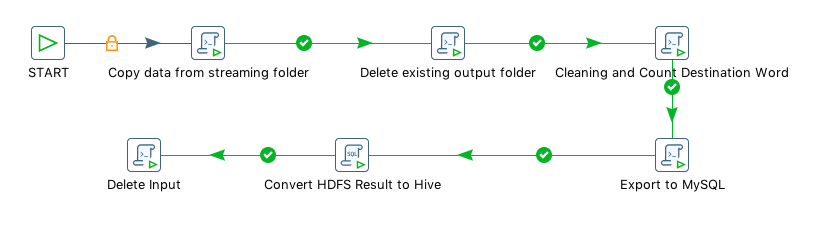
\includegraphics[scale=0.5]{Gambar/ui-implementation-pentaho-di.png}
	\caption[Implementasi ETL Job pada Pentaho Data Integration]{Implementasi ETL Job pada Pentaho Data Integration} 
	\label{fig:ui_implementation_pentaho_di}
\end{figure}

\subsection{Implementasi Modul Program Sistem Kecerdasan Bisnis}
Implementasi modul program sistem kecerdasan bisnis akan terbagi menjadi tiga buah bagian yaitu implementasi antarmuka program \textit{client} dan implementasi kode di sisi \textit{client} dan \textit{server}. 

\subsubsection{Implementasi Antarmuka Sistem Kecerdasan Bisnis}
Terdapat dua buah antarmuka yang diimplementasikan pada penelitian ini. Antarmuka yang pertama adalah antarmuka untuk halaman \textit{dashboard}. Pada halaman ini pengguna dapat melihat situasi tren lokasi wisata terkini. Gambar \ref{fig:ui_implementasi_bi_dashboard_1} menggambarkan kondisi awal ketika \textit{dashboard} diakses dan Gambar \ref{fig:ui_implementasi_bi_dashboard_2} menggambarkan kondisi \textit{drill down} ketika map dan diagram-diagram diklik.

\begin{figure}[H]
	\centering
	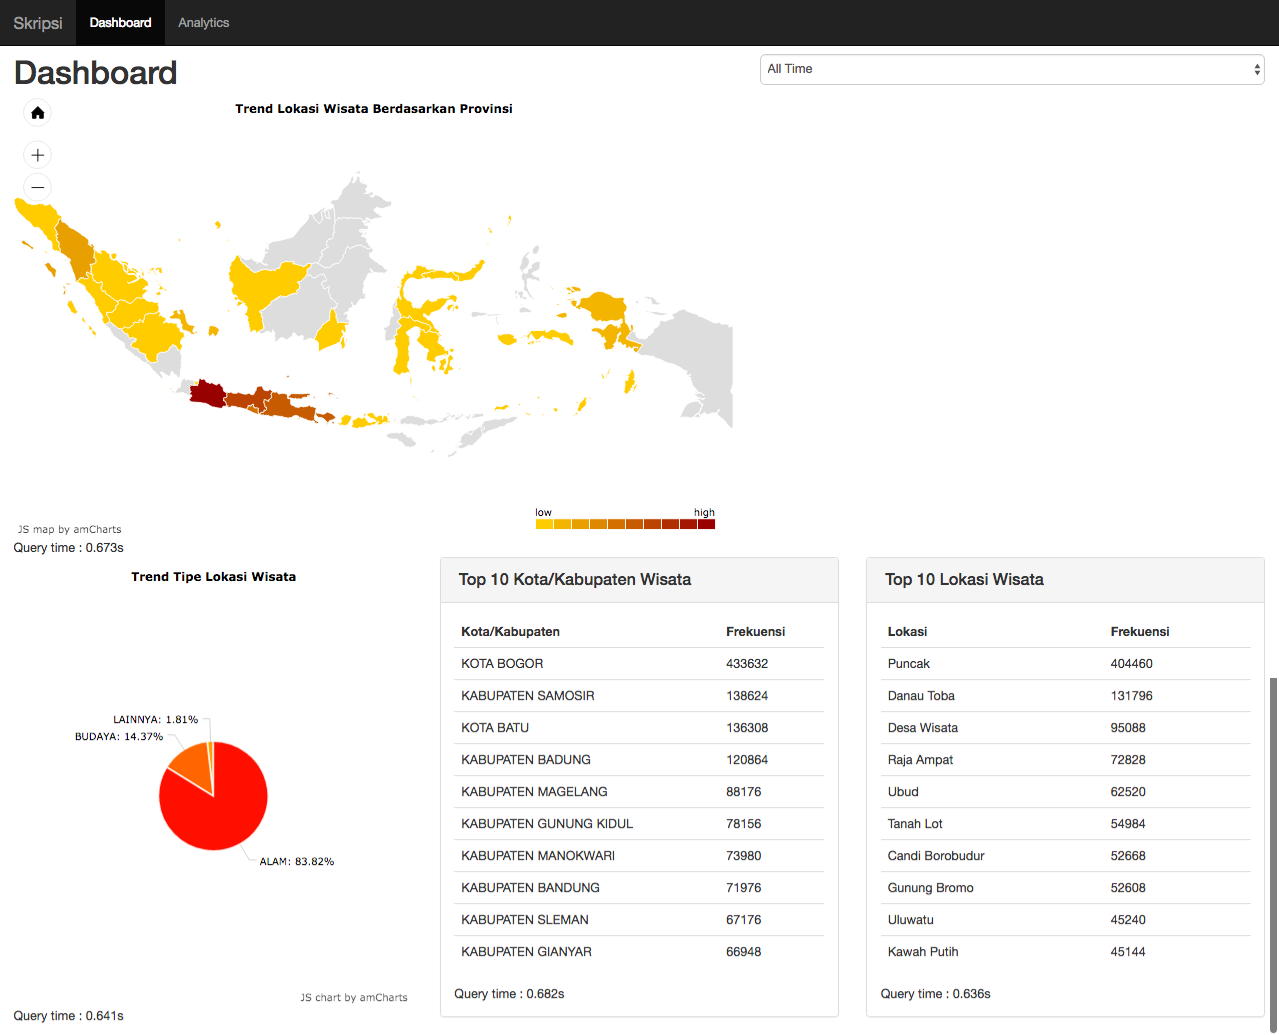
\includegraphics[scale=0.35]{Gambar/ui-implementasi-bi-dashboard-01.png}
	\caption[Implementasi Antarmuka Dashboard Sistem Kecerdasan Bisnis]{Implementasi Antarmuka Dashboard Sistem Kecerdasan Bisnis} 
	\label{fig:ui_implementasi_bi_dashboard_1}
\end{figure}

\begin{figure}[H]
	\centering
	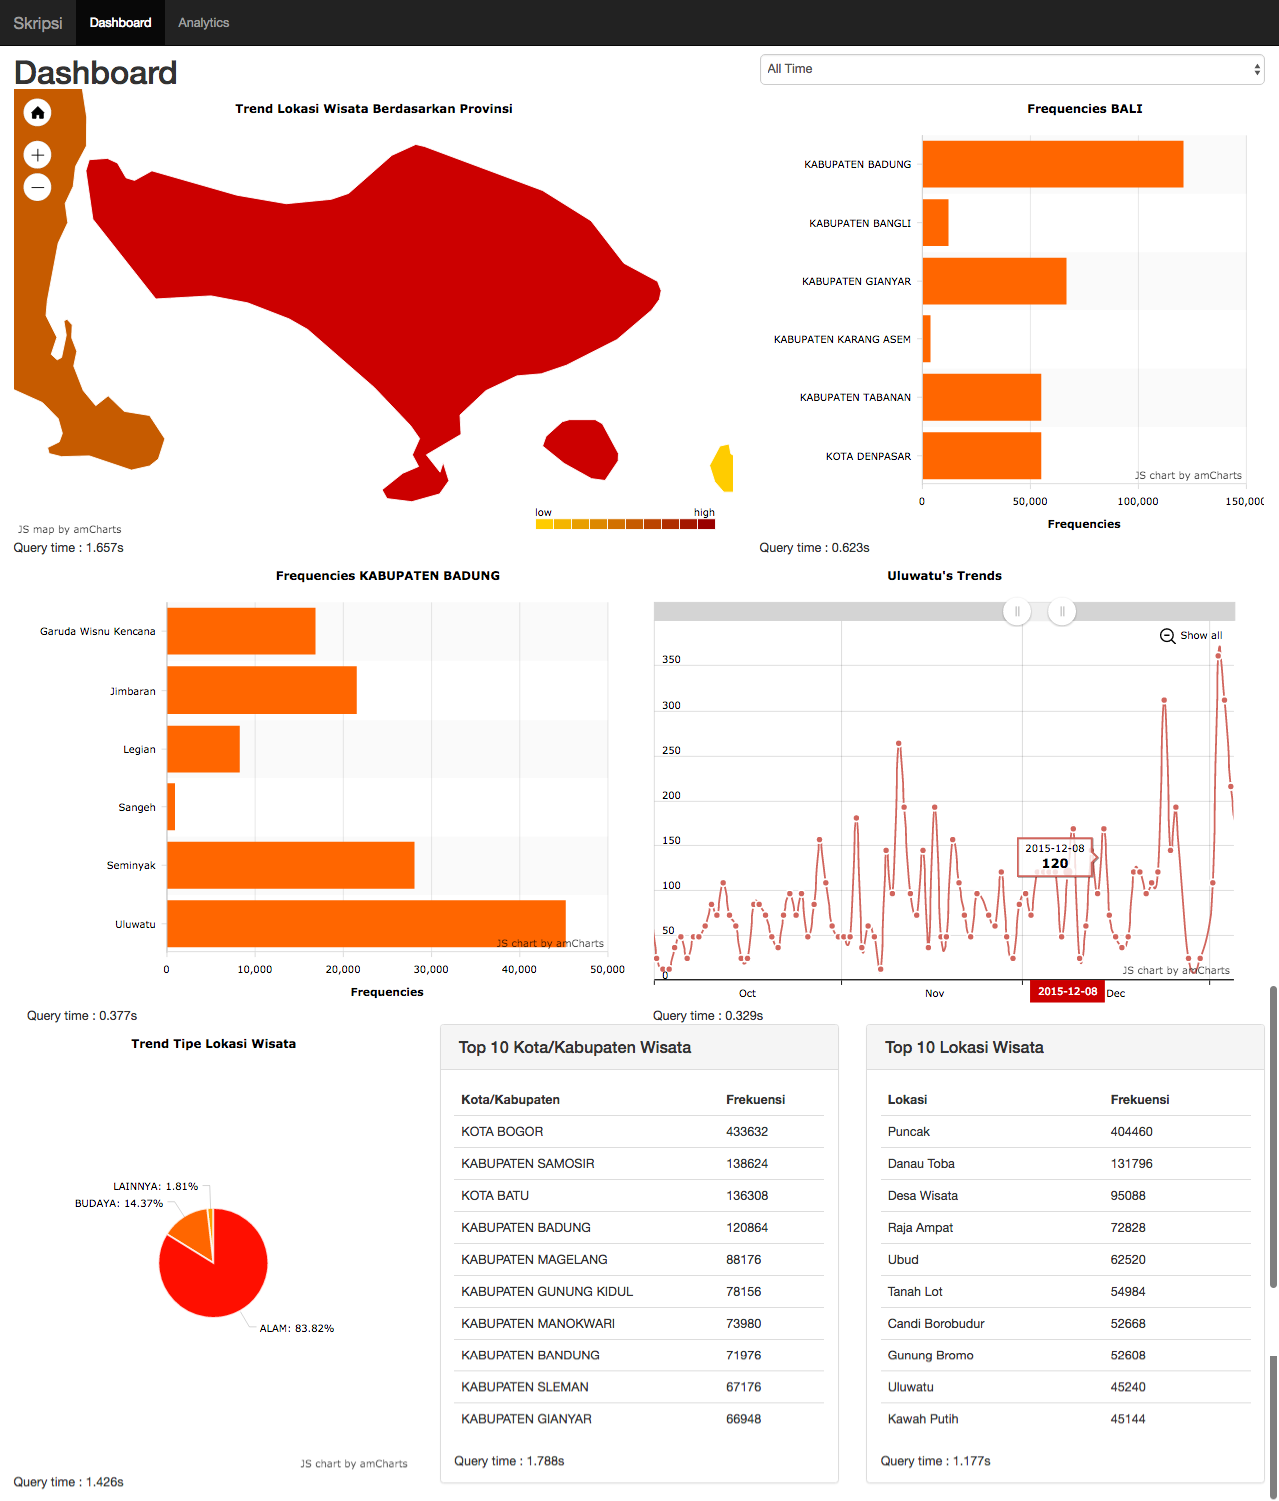
\includegraphics[scale=0.35]{Gambar/ui-implementasi-bi-dashboard-02.png}
	\caption[Implementasi Antarmuka Dashboard Sistem Kecerdasan Bisnis Ketika \textit{Drill Down}]{Implementasi Antarmuka Dashboard Sistem Kecerdasan Bisnis Ketika \textit{Drill Down}} 
	\label{fig:ui_implementasi_bi_dashboard_2}
\end{figure}

Antarmuka yang kedua adalah antarmuka untuk halaman pelaporan dan analisis. Pada halaman ini pengguna dapat memilih sumber data \textit{cube} yang hendak digunakan. Kemudian pengguna dapat melihat laporan dari berbagai sudut dimensi dan \textit{measure}. Terdapat juga pilihan untuk pengurutan data dan pembatasan jumlah data yang dicari. Pengguna juga bisa memasukan kriteria-kriteria yang diperlukan pada bagian \textit{filter} atau \textit{having}.

Tampilan data yang dihasilkan pada modul program ini dapat berupa tabel, diagram batang, diagram baris atau pun diagram pie. Contoh-contoh hasil tampilan data dari modul program ini terdapat pada Gambar \ref{fig:ui_implementasi_bi_reporting_1}, \ref{fig:ui_implementasi_bi_reporting_2}, dan \ref{fig:ui_implementasi_bi_reporting_3}.

\begin{figure}[H]
	\centering
	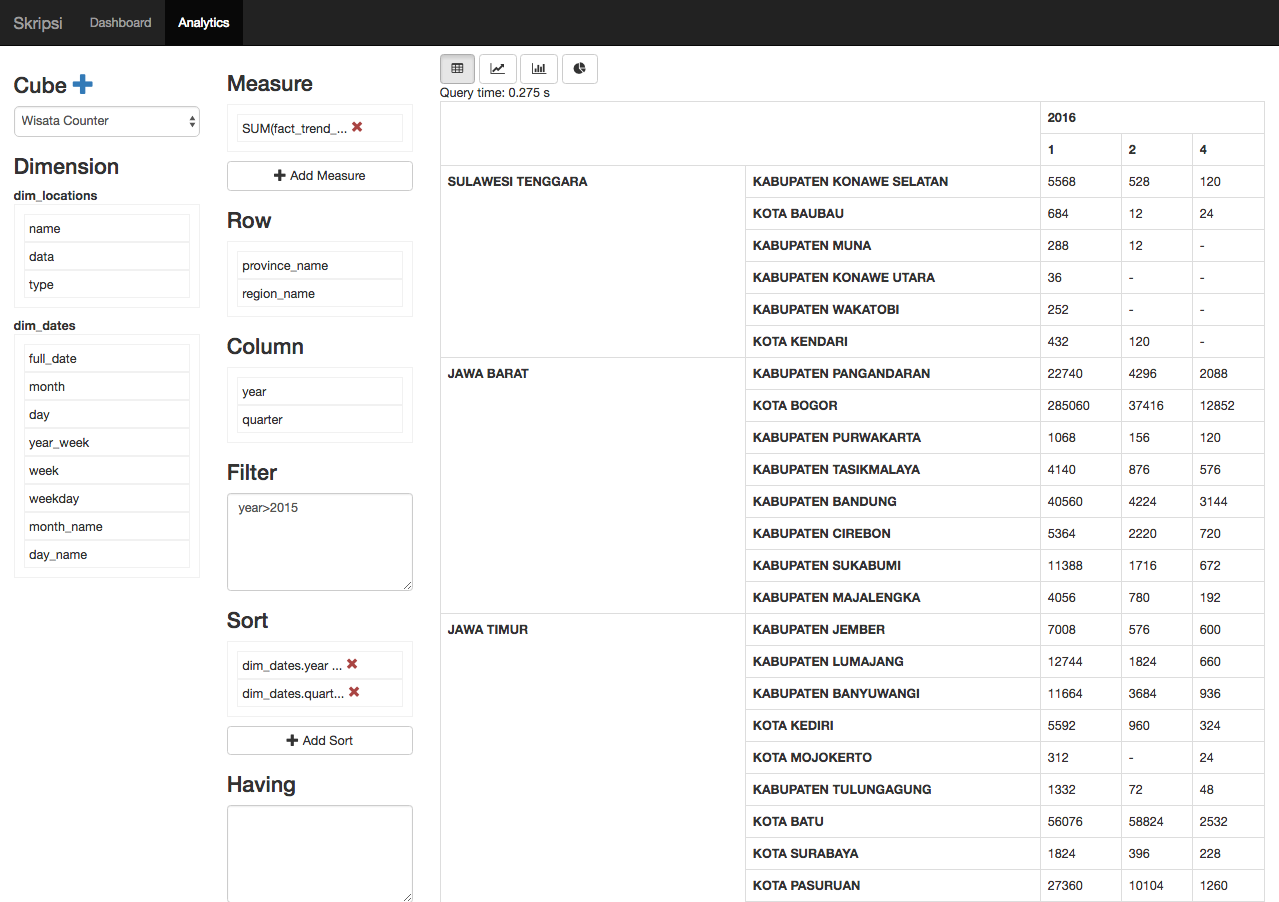
\includegraphics[scale=0.35]{Gambar/ui-implementasi-bi-reporting-01.png}
	\caption[Implementasi Antarmuka Tabel Pelaporan dan Analisis Sistem Kecerdasan Bisnis]{Implementasi Antarmuka Tabel Pelaporan dan Analisis Sistem Kecerdasan Bisnis} 
	\label{fig:ui_implementasi_bi_reporting_1}
\end{figure}

\begin{figure}[H]
	\centering
	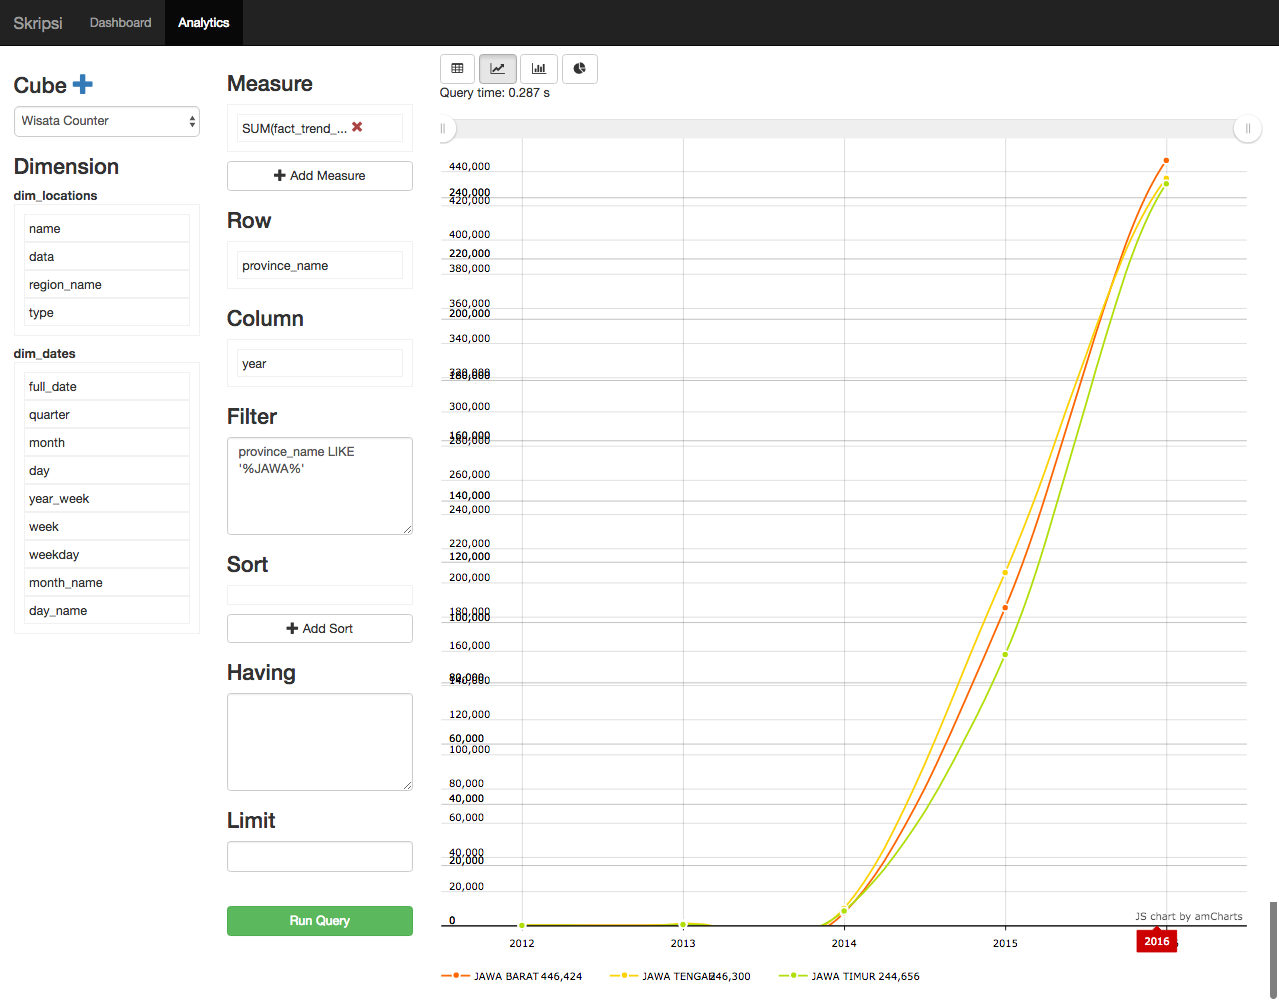
\includegraphics[scale=0.35]{Gambar/ui-implementasi-bi-reporting-02.png}
	\caption[Implementasi Antarmuka Grafik Pelaporan dan Analisis Sistem Kecerdasan Bisnis]{Implementasi Antarmuka Grafik Pelaporan dan Analisis Sistem Kecerdasan Bisnis} 
	\label{fig:ui_implementasi_bi_reporting_2}
\end{figure}

\begin{figure}[H]
	\centering
	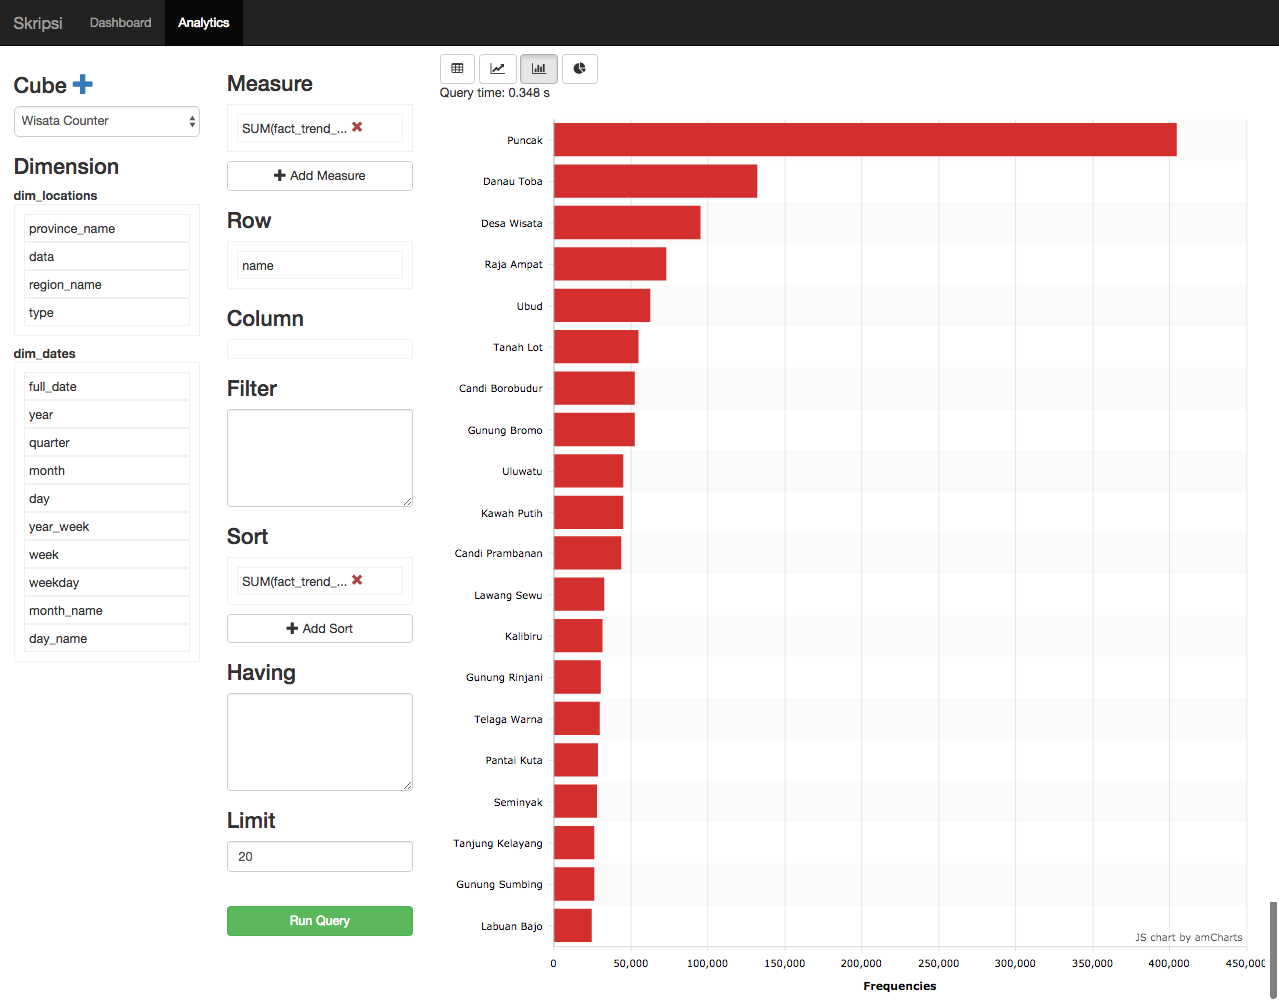
\includegraphics[scale=0.35]{Gambar/ui-implementasi-bi-reporting-03.png}
	\caption[Implementasi Antarmuka Grafik Pelaporan dan Analisis Sistem Kecerdasan Bisnis]{Implementasi Antarmuka Grafik Pelaporan dan Analisis Sistem Kecerdasan Bisnis} 
	\label{fig:ui_implementasi_bi_reporting_3}
\end{figure}

\subsubsection{Implementasi Kode Program Sistem Kecerdasan Bisnis}
Kode program pada sistem kecerdasan bisnis yang dibangun dibagi menjadi dua bagian. Bagian yang pertama adalah kode program di sisi \textit{client}, kode program pada bagian ini dibuat menggunakan HTML5, CSS, Javascript dan AMChart. Bagian yang kedua adalah kode program di sisi \textit{server}, kode program pada bagian ini dibuat dalam bahasa pemrograman Java dengan memanfaatkan Java servlet untuk melayani \textit{request} dan \textit{response} dari program \textit{client} via HTTP. 

Listing \ref{lst:kode_bi_client_dashboard_1}, \ref{lst:kode_bi_client_dashboard_2} dan \ref{lst:kode_bi_client_reporting_1} adalah potongan-potongan kode program dalam bahasa Javascript yang berjalan di sisi \textit{client}. Listing \ref{lst:kode_bi_client_dashboard_1} berfungsi untuk melakukan \textit{request} ke server kemudian menampilkan hasilnya ke dalam bentuk map menggunakan kode program pada Listing \ref{lst:kode_bi_client_dashboard_2}. Listing \ref{lst:kode_bi_client_reporting_1} berfungsi untuk mengirimkan \textit{request} ke server sesuai dengan kueri yang diinginkan oleh pengguna, \textit{response} pada listing ini akan ditampilkan dalam bentuk tabel.

Listing \ref{lst:kode_bi_server_reporting_1}, \ref{lst:kode_bi_server_reporting_2} dan \ref{lst:kode_bi_server_reporting_3} adalah potongan-potongan kode program di sisi server yang ditulis dalam bahasa Java. Listing \ref{lst:kode_bi_server_reporting_1} bertugas membuat koneksi ke sumber data, yaitu MySQL atau Hive. Listing \ref{lst:kode_bi_server_reporting_2} berfungsi untuk mengambil data dari \textit{connection file} lalu melakukan koneksi ke sumber data sesuai dengan konfigurasi di \textit{connection file}. Sedangkan pada Listing \ref{lst:kode_bi_server_reporting_3} berfungsi untuk membuat kueri-kueri yang sesuai dengan masukan dari pengguna.

\begin{lstlisting}[language=HTML,basicstyle=\tiny,caption=script-dasboard.js (Dashboard),label={lst:kode_bi_client_dashboard_1}]
....

$(function(){
    ....
    
    //load ajax
    var rowAttrs = "dim_locations.province_name,";
    var columnAttrs = "";
    var aggregate = "SUM(fact_trend_locations.qty),";
    var condition = "";
    var sort = "";
    var limit = 0;
    var having = "";

    $.ajax({
        method: "POST",
        url: baseUrl + "/generator",
        data: {rowAttrs: rowAttrs, columnAttrs: columnAttrs, aggregate: aggregate, condition: condition, sort: sort, limit: limit, having: having, connectionId: 1, cubeId: 0},
        success: function(data){
            globalMapData = data;
            createMap();
        },
        beforeSend: function(){
            $("#map").html("Loading...");
        }
    });
    
    ....
});

....
\end{lstlisting}

\begin{lstlisting}[language=HTML,basicstyle=\tiny,caption=script-dasboard.js (Dashboard),label={lst:kode_bi_client_dashboard_2}]
....
function createMap(){
    var areas = [];

    for (var i = 0; i < globalMapData.data.length; i++) {
        var data = globalMapData.data[i];
        var value = {};
        value['id'] = globalMaps[data.rows[0]];
        value['value'] = data.values[0];
        areas.push(value);
    }

    var map = new AmCharts.AmMap();
    map.titles = [{"text" : "Trend Lokasi Wisata Berdasarkan Provinsi"}]
    map.colorSteps = 10;
    map.dataProvider = {
        map: "indonesiaHigh",
        areas: areas
    };
    map.areasSettings = {
        autoZoom: true
    };
    map.imagesSettings.balloonText = "<span style='font-size:14px;'><b>[[title]]</b>: [[value]]</span>";

    var valueLegend = new AmCharts.ValueLegend();
    valueLegend.right = 20;
    valueLegend.minValue = "low";
    valueLegend.maxValue = "high";
    map.valueLegend = valueLegend;

    map.addListener("clickMapObject", clickGraph);
    map.write("map");

    $("#map-query-time").html("Query time : " + globalMapData.query_time / 1000 + "s");
}
....
\end{lstlisting}

\begin{lstlisting}[language=HTML,basicstyle=\tiny,caption=script.js (Membuat \textit{request} ke \textit{server} - Laporan dan Analisis),label={lst:kode_bi_client_reporting_1}]
....
$("#run-query").click(function(){
    var rowAttrs = "";
    var columnAttrs = "";
    var aggregate = "";
    var sort = "";
    var limit = 0;

    //get from measure
    $("#measure-sortable li").each(function(){
        aggregate += $(this).data("column") + ",";
    });

    //get from row
    $("#row-sortable li").each(function(){
        rowAttrs += $(this).data("column") + ",";
    });

    //get from column
    $("#column-sortable li").each(function(){
        columnAttrs += $(this).data("column") + ",";
    });

    //get sorting
    $("#sort-sortable li").each(function(){
        sort += $(this).data("column") + ",";
    });

    //get selected cube
    var option = $("#connection-select").find(":selected");

    //get limit
    if($("#limit").val() != "" && $("#limit").val() != 0){
        limit = $("#limit").val();
    }

    $.ajax({
        method: "POST",
        url: baseUrl + "/generator",
        data: {rowAttrs: rowAttrs, columnAttrs: columnAttrs, aggregate: aggregate, condition: $("#filter").val(), having: $("#having").val(), limit: limit, sort: sort, connectionId: option.data("connection"), cubeId: option.data("cube")},
        success: function(data){
       		if(data.data.length > 0){
                globalData = data;

                var resultOption = $("#result-option").find(".active").data("type");

                if(resultOption == "bar"){
                    createBarChart();
                }else if(resultOption == "line"){
                    createLineChart();
                }else if(resultOption == "table"){
                    generateTable();
                }else if(resultOption == "pie"){
                    createPieChart();
                }
            }else{
                $("#query-time").html("Query time: " + data.query_time / 1000 + "s");
                $("#result-area").html("No data found.");
            }
        },
        beforeSend: function(){
            $("#result-area").html("");
            $("#query-time").html("Loading...");
        }
    })
});
....
\end{lstlisting}

\begin{lstlisting}[language=Java,basicstyle=\tiny,caption=DbConnection.java,label={lst:kode_bi_server_reporting_1}]
public class DbConnection {
	....
	
    private static Connection con;
    
    public static Connection getConnection(String host, String user, String pass, int port, String db, String driver){
        try {
            String url = "";

            switch(driver){
                case "com.mysql.jdbc.Driver":
                    url = "jdbc:mysql://" + host + ":" + port + "/" + db + "";
                    break;
                case "org.apache.hive.jdbc.HiveDriver":
                    url = "jdbc:hive2://" + host + ":" + port + "/" + db + "";
                    break;
            }

            Class.forName(driver).newInstance();
            DbConnection.con = (Connection) DriverManager.getConnection(url, user, pass);
        } catch (Exception ex) {
            Logger.getLogger(DbConnection.class.getName()).log(Level.SEVERE, null, ex);
        } 
        
        return DbConnection.con;
    }
}
\end{lstlisting}

\begin{lstlisting}[language=Java,basicstyle=\tiny,caption=ConnectionReaderWriter.java,label={lst:kode_bi_server_reporting_2}]
public class ConnectionReaderWriter {
	... 
	
	public String getCubeDetail(int connectionId, int cubeId){
        try {
            JSONArray connections = new JSONArray(this.getConnections());
            JSONObject connection = (new JSONObject(this.getConnection(connectionId))).getJSONObject("connection");
            JSONObject cube = connections.getJSONObject(connectionId).getJSONArray("cubes").getJSONObject(cubeId);
            JSONArray dims = cube.getJSONArray("dim");
            
            String host = connection.getString("host");
            String user = connection.getString("username");
            String pass = connection.getString("password");
            String db = connection.getString("database");
            int port = connection.getInt("port");
            String driver = connection.getString("driver");
            
            conn = DbConnection.getConnection(host, user, pass, port, db, driver);
            String table = cube.getString("fact");
            
            //init json object as parent
            JSONObject json = new JSONObject();
            
            //fetch fact data
            JSONObject tableNodeJson = new JSONObject();
            tableNodeJson.put("name", table);
            tableNodeJson.put("columns", this.getColumn(table));            
            json.put("fact", tableNodeJson);
            
            //fetch dim data
            JSONArray dimsJson = new JSONArray();
            for (int i = 0; i < dims.length(); i++) {
                table = dims.getJSONObject(i).getString("table");
                tableNodeJson = new JSONObject();
                tableNodeJson.put("name", table);
                tableNodeJson.put("columns", this.getColumn(table)); 
                dimsJson.put(tableNodeJson);
            }
            json.put("dims", dimsJson);
            
            return json.toString();
        } catch (JSONException ex) {
            Logger.getLogger(ConnectionReaderWriter.class.getName()).log(Level.SEVERE, null, ex);
        } catch (IOException ex) {
            Logger.getLogger(ConnectionReaderWriter.class.getName()).log(Level.SEVERE, null, ex);
        } catch (SQLException ex) {
            Logger.getLogger(ConnectionReaderWriter.class.getName()).log(Level.SEVERE, null, ex);
        } 
        
        return null;
    }
    
    ...
}
\end{lstlisting}

\begin{lstlisting}[language=Java,basicstyle=\tiny,caption=QueryBuilder.java,label={lst:kode_bi_server_reporting_3}]
public class QueryBuilder {
    ....
    public String create(String rowAttrs, String columnAttrs , String aggregate, String condition, String order, int limit, String having){
        /**
         * SELECT ..., ..., SUM(...)
         * FROM fact
         * JOIN dim ON relation
         * JOIN dim ON relation
         * JOIN dim ON relation
         * WHERE ...
         * ORDER BY ... ASC
         * GROUP BY ..., ...
         */
        //set global so other methods can use it
        String attrs = (rowAttrs + columnAttrs);
        this.rowAttrs = rowAttrs;
        this.columnAttrs = columnAttrs;
        this.aggregate = aggregate;
        String sql = "SELECT ";
        //create select query
        sql += rowAttrs + columnAttrs;
        //create aggregate function
        sql += aggregate.substring(0, aggregate.length() - 1) + " ";
        //create from query
        sql += from + " ";
        //create join query
        sql += join + " ";
        //create where query
        if(condition != null && !condition.isEmpty()){
            sql += "WHERE " + condition + " ";
        }
        //create group query
        sql += "GROUP BY " + attrs.substring(0, attrs.length() - 1) + " ";
        
        if(having != null && !having.isEmpty()){
            sql += "HAVING " + having + " ";
        }
        
        //create order query
        if(!order.isEmpty()){
            sql += "ORDER BY " + order.substring(0, order.length() - 1) + " ";
        }
        if(limit != 0){
            sql += "LIMIT " + limit + " ";
        }
        
        return sql;
    }
    ....
}
\end{lstlisting}

\section{Pengujian Modul Program}
Pada sub bab ini, modul-modul program yang sudah dibuat akan diuji kebenaran berdasarkan masukan dan keluaran dari program. Tujuan dari pengujian ini adalah untuk memastikan bahwa setiap modul program sudah berjalan dengan benar sesuai dengan perancangan. Modul-modul program yang akan diuji adalah modul program untuk melakukan \textit{streaming} ke Twitter, \textit{crawling} Instagram serta modul program untuk menghitung tren lokasi wisata baik dengan MapReduce maupun tanpa MapReduce),.

\subsection{Pengujian Modul Program \textit{Streaming} Twitter}
Pengujian ini dilakukan untuk memastikan modul program yang dibuat dapat mengambil data dari Twitter Streaming API, serta menulis hasilnya ke HDFS. Pengujian ini di awali dengan memasukan consumer key, consumer secret, access token, dan access token secret yang didapat ketika mendaftarkan aplikasi di Twitter Streaming API. Kemudian dimasukan \textit{keyword-keyword} yang sesuai, yaitu libur, liburan, travel, travelling, wisata, tour, pariwisata, destinasi, jalan-jalan, hotel, pesawat, cruise, jelajah, petualangan. Untuk pilihan destinasi file dipilih HDFS dan diarahkan ke dalam path /wilianto/testing. 

\begin{figure}[H]
	\centering
	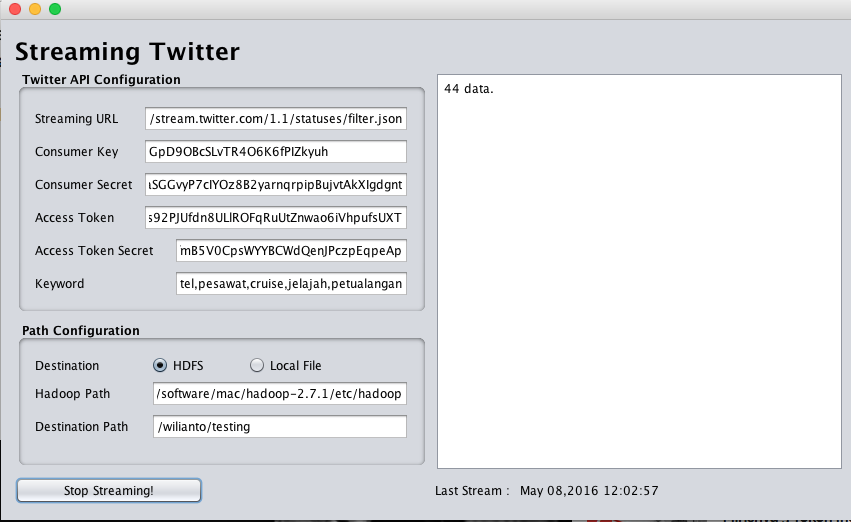
\includegraphics[scale=0.5]{Gambar/testing-twitter-01.png}
	\caption[Antar muka modul program ketika berjalan]{Antar muka modul program ketika berjalan} 
	\label{fig:testing_twitter_01}
\end{figure}

Setelah terisi maka \textit{streaming} ke Twitter dapat dilakukan. Tampilan antar muka program ketika sedang berproses dapat dilihat di Gambar \ref{fig:testing_twitter_01}. Hasil keluaran dari program di HDFS dapat dilihat pada Gambar \ref{fig:testing_twitter_02}. Berdasarkan pengujian ini maka, dapat disimpulkan modul program \textit{streaming} Twitter sudah berjalan dengan baik dan sesuai perancangan.

\begin{figure}[H]
	\centering
	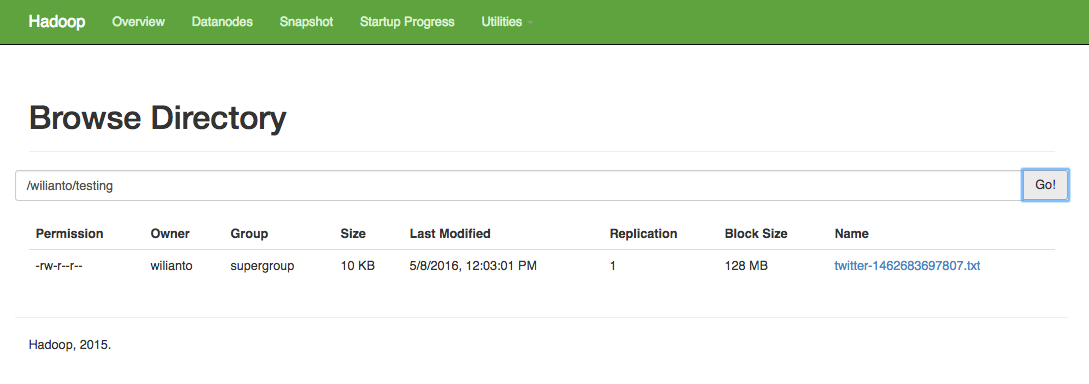
\includegraphics[scale=0.4]{Gambar/testing-twitter-02.png}
	\caption[Hasil keluaran dari modul program di HDFS]{Hasil keluaran dari modul program di HDFS} 
	\label{fig:testing_twitter_02}
\end{figure}

\subsection{Pengujian Modul Program \textit{Crawling} Instagram}
Pengujian ini dilakukan untuk memastikan modul program yang dibuat dapat mengambil data dari Instagram API, serta menulis hasilnya ke HDFS. Pengujian ini di awali dengan memasukan client ID, client secret dan redirect URL yang didapat ketika mendaftarkan aplikasi di Instagram API. Masukan berikutnya adalah code, untuk mendapatkan code pengguna harus mengklik tombol Get Code terlebih dahulu. Ketika tombol diklik, pengguna akan diarahkan ke browser dan diminta untuk melakukan autentikasi. Jika autentikasi berhasil dilakukan dan izin diberikan ke aplikasi, maka code akan diberikan. Pada masukan Next Min ID dapat dikosongkan apabila crawling ingin dilakukan dari data terbaru, sedangkan untuk melanjutkan dapat diisi dengan Next Min ID data awal. Tag yang diambil pada proses pengujian ini adalah exploreindonesia. Untuk pilihan destinasi file dipilih HDFS dan diarahkan ke dalam path /wilianto/testing. 

\begin{figure}[H]
	\centering
	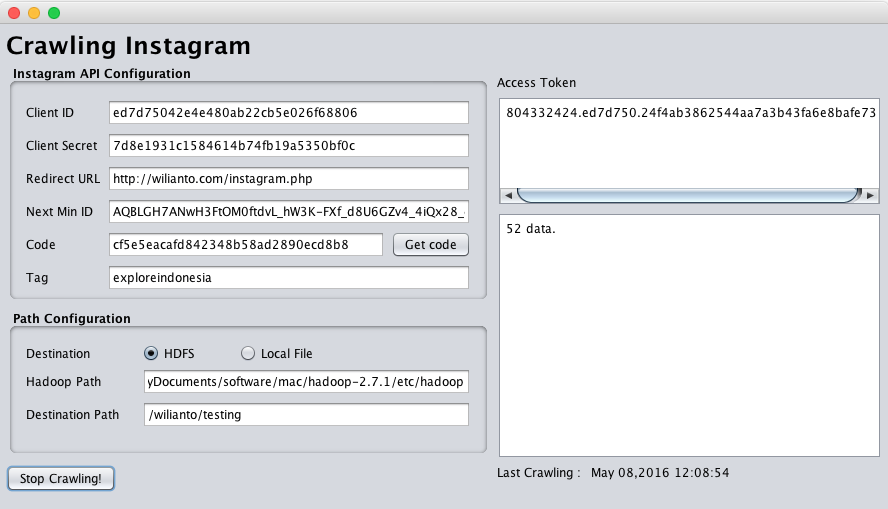
\includegraphics[scale=0.5]{Gambar/testing-instagram-01.png}
	\caption[Antar muka modul program ketika berjalan]{Antar muka modul program ketika berjalan} 
	\label{fig:testing_instagram_01}
\end{figure}

Setelah terisi maka \textit{crawling} ke Instagram dapat dilakukan. Tampilan antar muka program ketika sedang berproses dapat dilihat di Gambar \ref{fig:testing_instagram_01}. Hasil keluaran dari program di HDFS dapat dilihat pada Gambar \ref{fig:testing_instagram_02}. Berdasarkan pengujian ini maka, dapat disimpulkan modul program \textit{crawling} Instagram sudah berjalan dengan baik dan sesuai perancangan.

\begin{figure}[H]
	\centering
	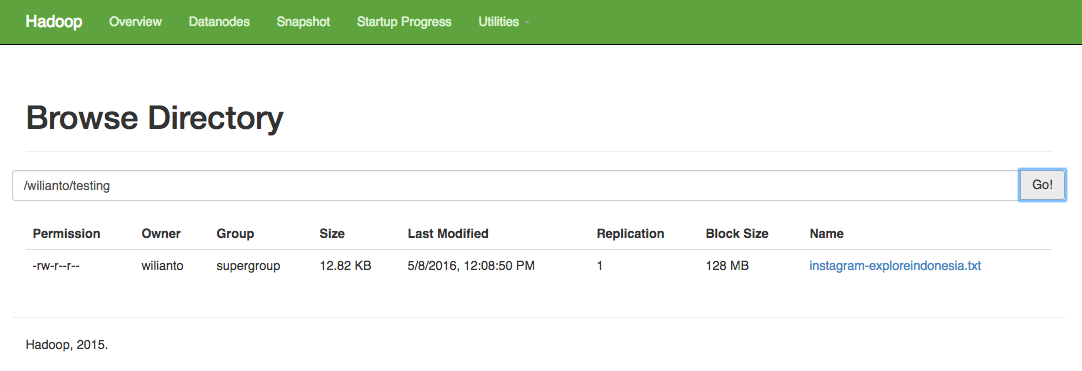
\includegraphics[scale=0.4]{Gambar/testing-instagram-02.png}
	\caption[Hasil keluaran dari modul program di HDFS]{Hasil keluaran dari modul program di HDFS} 
	\label{fig:testing_instagram_02}
\end{figure}

\subsection{Pengujian Modul Pembersihan Data dan Penghitungan Frekuensi Lokasi Wisata}
Pengujiannya dilakukan untuk memastikan modul program yang dibuat dapat melakukan pembersihan data dengan benar dan menghitung jumlah frekuensi kemunculan kata di dalam isi pesan sosial media (di kolom ke dua). Pada modul ini akan dilakukan pengujian dengan cara memasukan \textit{input} teks sosial media yang sudah dihitung secara manual jumlah kemunculan katanya. Lalu hasil keluaran dari program akan dicocokan dengan hasil perhitungan manual yang dilakukan. Hasil dari perhitungan manual dapat dilihat pada Tabel \ref{tab:hasil_hitung_manual} dan data input dapat dilihat pada Lampiran \ref{app:I}.

\begin{table}[!htb]
	\centering
	\begin{tabular}{| l | l | c |}
		\hline
		Lokasi & Tanggal & Frekuensi \\
	 	\hline
	 	candi borobudur & 2016-03-07 & 1\\
		candi borobudur & 2016-05-08 & 3\\
		dunia fantasi & 2016-05-08 & 2\\
		kawah putih & 2016-05-08 & 3\\
		pantai pangandaran & 2016-03-07 & 1\\
		pantai pangandaran & 2016-05-08 & 1\\
		pantai sanur & 2016-05-07 & 2\\
		pantai sanur & 2016-05-08 & 3\\
		pulau samosir & 2016-05-07 & 1\\
		pulau samosir & 2016-05-08 & 1\\
		pura besakih & 2016-05-08 & 1\\
		tanah lot & 2016-05-08 & 3\\
		tomok & 2016-05-08 & 1\\
		uluwatu & 2016-05-07 & 1\\
		uluwatu & 2016-05-08 & 1\\
	 	\hline
	\end{tabular}	
	\caption{Hasil Perhitungan Manual}\label{tab:hasil_hitung_manual}
\end{table}	

Hasil keluaran dari kedua program untuk pengujian ini dapat dilihat pada Gambar \ref{fig:counter_mp_output} untuk keluaran program dengan MapReduce dan Gambar \ref{fig:counter_single_output} untuk keluaran program tanpa MapReduce. Dari kedua keluaran dapat dilihat bahwa hasilnya sudah sesuai dengan perhitungan manual yang dilakukan. Oleh karena ini dapat ditarik kesimpulan bahwa modul program ini sudah berjalan dengan baik dan sesuai dengan perancangan.

\begin{figure}[H]
	\centering
	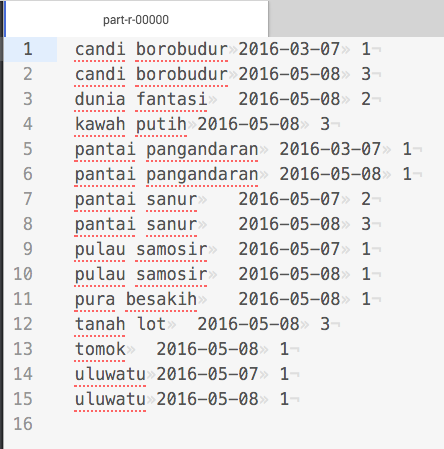
\includegraphics[scale=0.5]{Gambar/counter-mp-output.png}
	\caption[Hasil keluaran dari modul program dengan MapReduce]{Hasil keluaran dari modul program dengan MapReduce} 
	\label{fig:counter_mp_output}
\end{figure}

\begin{figure}[H]
	\centering
	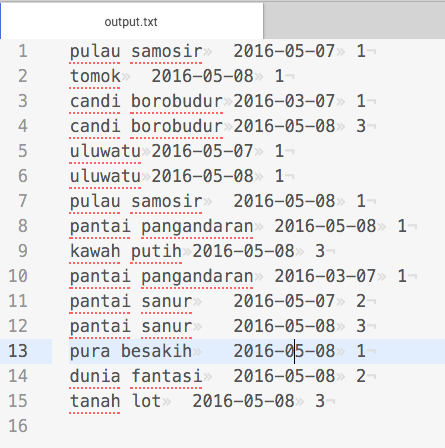
\includegraphics[scale=0.5]{Gambar/counter-single-output.png}
	\caption[Hasil keluaran dari modul program tanpa MapReduce]{Hasil keluaran dari modul program tanpa MapReduce} 
	\label{fig:counter_single_output}
\end{figure}

\section{Eksperimen}
Pengujian waktu eksekusi program dilakukan untuk mengukur kecepatan program dalam menyelesaikan masalah. Pengujian dilakukan pada dua modul program yang berbeda, yaitu modul program untuk pembersihan dan menghitung frekuensi kemunculan lokasi wisata. Pengujian kedua dilakukan pada modul program sistem kecerdasan bisnis untuk menghitung kecepatan kueri-kueri yang dibuat.

Dalam melakukan pengujian, penguji menggunakan komputer-komputer di dalam laboratorium sesuai dengan spesifikasi yang sudah dijelaskan pada Bab \ref{sec:deskripsi_perangkat_keras}. Terdapat dua buah pengujian yang dilakukan untuk modul program pembersihan dan menghitung frekuensi, yaitu pengaruh ukuran blok terhadap waktu eksekusi dan pengaruh jumlah node terhadap waktu eksekusi.

\subsection{Uji Pengaruh Ukuran Blok terhadap Kecepatan}
Pengujian pengaruh ukuran blok terhadap waktu dilakukan dengan spesifikasi seperti berikut: 
\begin{itemize}
	\item Jumlah node: 25 node
	\item Ukuran data: 10.98 GB (terdiri dari data tweet dan caption instagram yang sudah diduplikasi)
\end{itemize}

\begin{table}
	\centering
	\begin{tabular}{| l | c | c | c | c | c | c |}
		\hline
		Block Size (MB)	& 1 & 2 & 3 & 4 & 5 & Rata-rata  \\
		\hline
		16 	& 122	& 119	& 118	& 118	& 117  & 118.8 \\
		32		& 88	& 84	& 83	& 87	& 82 & 84.8\\
		64		& 67	& 65	& 67	& 66	& 65 & 66\\
		128	& 66	& 59	& 61	& 57	& 58 & 60.2\\
		\hline
	\end{tabular}	
	\caption{Hasil uji pengaruh ukuran blok terhadap kecepatan dalam detik} \label{tab:waktu_blok}
\end{table}	

Gambar \ref{fig:eks_block_size} memperlihatkan grafik rata-rata waktu ekskusi. Dari grafik dapat dilihat bahwa ukuran blok memiliki pengaruh terhadap waktu eksekusi program. Waktu eksekusi tercepat adalah pada ukuran blok 128 MB.

\begin{figure}[H]
	\centering
	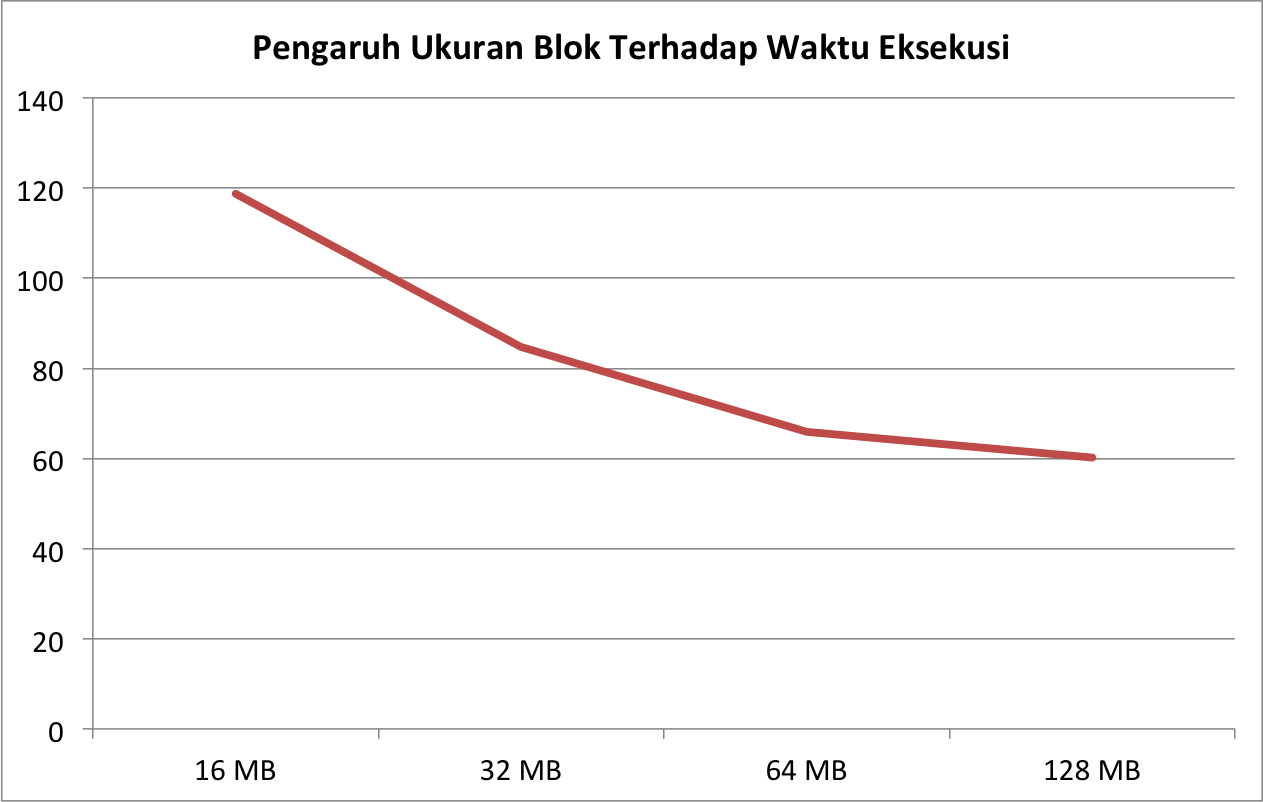
\includegraphics[scale=0.5]{Gambar/eks-block-size.png}
	\caption[Grafik pengaruh ukuran blok terhadap rata-rata waktu eksekusi]{Grafik pengaruh ukuran blok terhadap rata-rata waktu eksekusi} 
	\label{fig:eks_block_size}
\end{figure}

\subsection{Uji Pengaruh Jumlah Node terhadap Kecepatan}
Pengujian berikutnya adalah pengujian pengaruh jumlah \textit{node} terhadap waktu eksekusi. Pada pengujian ini, jumlah \textit{node} yang digunakan adalah kelipatan 5, dimulai dengan 1 node terlebih dahulu. Selain itu pengujian kali ini menguji performa modul program tanpa MapReduce. Hasil pengujian tertera pada Tabel \ref{tab:waktu_node}. Spesifikasi komputer-komputer yang digunakan pada pengujian ini adalah:
\begin{itemize}
	\item Jumlah node: mulai dari 1 hingga 25 
	\item Ukuran data: 10.98 GB (terdiri dari data tweet dan caption instagram yang sudah diduplikasi)
	\item Ukuran blok: 128 MB
\end{itemize}

\begin{table}
	\centering
	\begin{tabular}{ | l | c | c | c | c | c | c |}
		\hline
		Jumlah Node	& 1 & 2 & 3 & 4 & 5 & Rata-rata  \\
		\hline
		Tanpa MapReduce & 958	& 953	& 955	& 950	& 948  & 952.8\\
		1	& 1015	& 1012	& 1005	& 1008	& 1010 & 1010\\
		5	& 210	& 202	& 201	& 200	& 201 & 202.8\\
		10	 & 120	& 113	& 112	& 117	& 119 & 116.2\\
		15	 & 99	 & 99 & 98	 & 97 	& 93  & 97.2\\
		20	 & 75	 & 77 & 80	 & 69	 & 70 & 74.2\\
		25	 & 66	 & 59	 & 61 & 57	 & 58 & 60.2\\
		\hline
	\end{tabular}	
	\caption{Hasil uji pengaruh jumlah node terhadap kecepatan program dalam detik}\label{tab:waktu_node}
\end{table}	

Pada Gambar \ref{fig:eks_node_size} terlihat bahwa jumlah \textit{node} memiliki dampak pada kecepatan waktu eksekusi.

\begin{figure}[H]
	\centering
	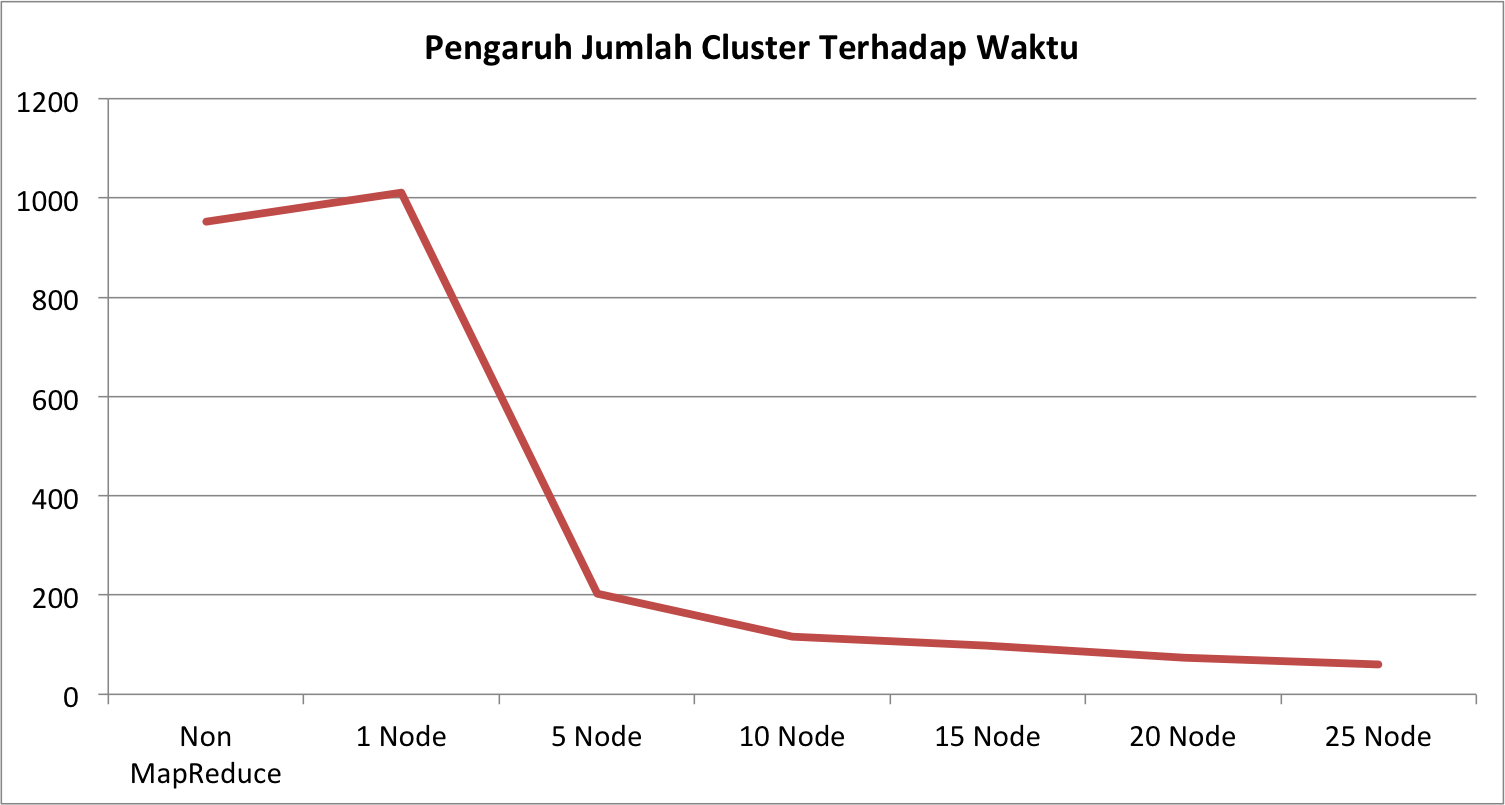
\includegraphics[scale=0.5]{Gambar/eks-node-size.png}
	\caption[Grafik pengaruh jumlah node terhadap rata-rata waktu eksekusi]{Grafik pengaruh jumlah node terhadap rata-rata waktu eksekusi} 
	\label{fig:eks_node_size}
\end{figure}

\subsection{Eksperimen Kueri}
Pengujian kedua dilakukan pada modul program sistem kecerdasan bisnis untuk menghitung kecepatan kueri-kueri yang dibuat. Pengujian dilakukan dengan membandingkan performa kueri yang dijalankan pada Hive dan pada MySQL. Pada pengujian ini digunakan komputer-komputer dengan spesifikasi sebagai berikut untuk menjalankan kueri-kueri di Hive.
\begin{itemize}
	\item Jumlah node: 25 
	\item Ukuran data: 32.867.328 (dengan duplikasi dari hasil keluaran MapReduce)
	\item Ukuran blok: 128 MB
	\item Processor: 3.3 GHz Intel Core i3
	\item RAM: 4 GB DDR3
	\item Sistem Operasi: Ubuntu 14.04 LTS
	\item Versi Java: 1.8.0\_45
\end{itemize}

Sedangkan untuk MySQL menggunakan sebuah komputer dengan spesifikasi sebagai berikut:
\begin{enumerate}
	\item Processor: 3.3 GHz Intel Core i3
	\item RAM: 4 GB DDR3
	\item Sistem Operasi: Ubuntu 14.04 LTS
	\item Versi Java: 1.8.0\_45
\end{enumerate}

Listing \ref{lst:kueri_1}, \ref{lst:kueri_2}, \ref{lst:kueri_3} dan \ref{lst:kueri_4} adalah kueri-kueri yang diuji.

\begin{lstlisting}[language=SQL,basicstyle=\tiny,caption=Mencari tren wisata per provinsi,label={lst:kueri_1}]
SELECT dim_locations.province_name,SUM(fact_trend_locations.qty) 
FROM fact_trend_locations 
INNER JOIN dim_locations ON dim_locations.name = fact_trend_locations.destination 
LEFT JOIN dim_dates ON dim_dates.full_date = fact_trend_locations.post_date  
GROUP BY dim_locations.province_name 
\end{lstlisting}

\begin{lstlisting}[language=SQL,basicstyle=\tiny,caption=Mencari tren suatu lokasi wisata dari bulan ke bulan,label={lst:kueri_2}]
SELECT dim_locations.name,dim_dates.year,dim_dates.month,SUM(fact_trend_locations.qty) 
FROM fact_trend_locations 
INNER JOIN dim_locations ON dim_locations.name = fact_trend_locations.destination 
LEFT JOIN dim_dates ON dim_dates.full_date = fact_trend_locations.post_date  
WHERE dim_locations.name='danau toba' 
GROUP BY dim_locations.name,dim_dates.year,dim_dates.month 
ORDER BY dim_dates.year ASC,dim_dates.month ASC 
\end{lstlisting}

\begin{lstlisting}[language=SQL,basicstyle=\tiny,caption=Mencari tren suatu lokasi wisata dari hari ke hari,label={lst:kueri_3}]
SELECT dim_locations.name,dim_dates.year,dim_dates.month,dim_dates.day,SUM(fact_trend_locations.qty) 
FROM fact_trend_locations 
INNER JOIN dim_locations ON dim_locations.name = fact_trend_locations.destination 
LEFT JOIN dim_dates ON dim_dates.full_date = fact_trend_locations.post_date  
WHERE dim_locations.name='danau toba' 
GROUP BY dim_locations.name,dim_dates.year,dim_dates.month,dim_dates.day 
ORDER BY dim_dates.year ASC,dim_dates.month ASC,dim_dates.day ASC 
\end{lstlisting}

\begin{lstlisting}[language=SQL,basicstyle=\tiny,caption=Mencari tren tipe lokasi wisata,label={lst:kueri_4}]
SELECT dim_locations.type,SUM(fact_trend_locations.qty) 
FROM fact_trend_locations 
INNER JOIN dim_locations ON dim_locations.name = fact_trend_locations.destination 
LEFT JOIN dim_dates ON dim_dates.full_date = fact_trend_locations.post_date  
GROUP BY dim_locations.type 
\end{lstlisting}

Hasil dari pengujian ini dapat dilihat pada Tabel \ref{tab:eks_kueri}. Terdapat perbedaan waktu eksekusi kueri pada Hive dan MySQL.

\begin{table}
	\centering
	\begin{tabular}{| l | c | c |}
		\hline
		Kueri	& MySQL & Hive  \\
		\hline
		Listing \ref{lst:kueri_1} & 138.88 & 70.928 \\
		Listing \ref{lst:kueri_2} & 115.308 & 100.361 \\
		Listing \ref{lst:kueri_3} & 120.752 & 55.067 \\
		Listing \ref{lst:kueri_4} & 155.535 & 50.743 \\
		\hline
	\end{tabular}	
	\caption{Waktu eksekusi kueri-kueri dalam detik}\label{tab:eks_kueri}
\end{table}	

\section{Kesimpulan Eksperimen}
Berdasarkan pengujian-pengujian yang telah dilakukan, maka dapat diambil kesimpulan sebagai berikut:

\begin{itemize}
	\item Ukuran blok berpengaruh pada performa kecepatan eksekusi dari program yang dijalakan. Oleh karena itu pemilihan ukuran blok yang tepat perlu dilakukan dengan baik, agar program yang dieksekusi dapat berjalan secara optimal.
	\item Jumlah \textit{node} sangat berpengaruh pada kecepatan eksekusi program. Program MapReduce menghasilkan performa yang lebih baik apabila jumlah \textit{node}-nya banyak. Sedangkan jika hanya 1 node saja, maka waktu eksekusi program MapReduce lebih lambat daripada program Java tanpa menggunakan MapReduce.
	\item Kueri-kueri yang dijalankan di Hive memiliki performa yang lebih cepat dibandingkan kueri-kueri yang dijalankan pada MySQL.
\end{itemize}}{}
\ifdefstring{\vbabf}{1}{\chapter{Kesimpulan dan Saran}

\section{Kesimpulan}
Banyak informasi yang tersimpan di dalam pesan-pesan sosial media. Salah satunya adalah informasi tentang tren lokasi wisata. Data tren ini dapat bermanfaat bagi para pemilik usaha di bidang pariwisata dalam pengambilan keputusan. Namun dalam memperoleh data tersebut diperlukan sebuah sistem yang dapat berjalan dengan cepat dan akurat, mengingat data dari sosial media yang ukurannya sangat besar dan pergerakannya sangat cepat. 

Pada penelitian ini telah berhasil dibangun sistem terdistribusi Hadoop untuk mengolah data-data dari sosial media tersebut untuk keperluan informasi tren lokasi wisata. Sistem yang dibuat ini dapat berjalan dengan baik dan cepat. Hal ini dapat dilihat pada pengujian modul program yang berhasil memberikan keluaran yang tepat dan dapat berjalan dengan lebih cepat dibandingkan program \textit{standalone}. Masukan untuk modul program ini didapatkan dari modul-modul program pendukung lainnya yang membantu pengambilan data yang relevan dari sosial media Twitter dan Instagram.

Selain dari sisi pengolahan data mentah, modul program kecerdasan bisnis yang dibangun dapat menganalisis keluaran-keluaran yang diekspor ke dalam basis data menggunakan Apache Sqoop. Basis data utama yang digunakan pada penelitian ini adalah Hive yang bekerja pada sistem terdistribusi Hadoop. Sedangkan untuk basis data pembanding digunakan MySQL. Hasil dari ekperimen membandingkan lama waktu eksekusi dapat disimpulkan bahwa Hive memiliki performa yang lebih baik untuk memproses data dengan ukuran besar.

Secara keseluruhan sistem kecerdasan bisnis yang dibangun pada penelitian ini diawali dengan proses pengambilan data dari sosial media Twitter dan Instagram. Data yang sudah diambil kemudian dimasukan ke dalam HDFS untuk diolah secara berkala menggunakan modul program yang berjalan di sistem distribusi Hadoop. Hasil keluaran dari program berupa lokasi wisata, tanggal dan frekuensi kemunculan lokasi wisata. Keluaran tersebut diekspor ke Hive menggunakan kueri yang sudah tersedia di Hive dan diekspor ke basis data di luar Hadoop, yaitu MySQL menggunakan Apache Sqoop. Hasil-hasil dari keluaran tersebut diolah menggunakan modul program kecerdasan bisnis untuk memperoleh informasi-informasi yang dibutuhkan. Seluruh rangkaian proses yang dilakukan, mulai dari pemrosesan data di HDFS hingga hasilnya diekspor ke Hive dan MySQL dilakukan secara otomatis dan berkala menggunakan modul ETL yang dibangun menggunakan Pentaho Data Integration.

\section{Saran Penelitian Lanjutan}
Agar penelitian ini dapat terus berkembang, berikut saran-saran yang diusulkan:
\begin{itemize}
	\item Penelitian ini dikembangkan lagi dengan menambahkan jenis-jenis analisis lainnya dengan menggunakan teknik penambangan data, seperti misalnya analisis sentimen terhadap suatu lokasi wisata.
	\item Penelitian ini dikembangkan lagi dengan memperluas cakupan data sosial media yang diambil, tidak terbatas hanya Twitter dan Instagram, tapi juga dapat diambil dari Facebook, Path atau sosial media lainnya.
\end{itemize}}{}
\ifdefstring{\vbabg}{1}{\chapter{Kesimpulan dan Saran}

\section{Kesimpulan}
Banyak informasi yang tersimpan di dalam pesan-pesan sosial media. Salah satunya adalah informasi tentang tren lokasi wisata. Data tren ini dapat bermanfaat bagi para pemilik usaha di bidang pariwisata dalam pengambilan keputusan. Namun dalam memperoleh data tersebut diperlukan sebuah sistem yang dapat berjalan dengan cepat dan akurat, mengingat data dari sosial media yang ukurannya sangat besar dan pergerakannya sangat cepat. 

Pada penelitian ini telah berhasil dibangun sistem terdistribusi Hadoop untuk mengolah data-data dari sosial media tersebut untuk keperluan informasi tren lokasi wisata. Berikut adalah kesimpulan-kesimpulan yang didapatkan dari hasil penelitian ini. 

\begin{itemize}
	\item Media sosial Twitter dan Instagram dapat dimanfaatkan untuk menunjang pengambilan keputusan di bidang usaha pariwisata. Salah satu pemanfaatannya adalah untuk mencari tren lokasi wisata yang sedang ramai dibicarakan para pengguna sosial media. Hal ini dapat berdampak pada keputusan strategis perusahaan dalam pengambilan keputusan.
	\item Secara keseluruhan sistem yang dibangun pada penelitian ini diawali dengan proses pengambilan data dari sosial media Twitter dan Instagram. Data yang sudah diambil kemudian dimasukan ke dalam HDFS untuk diolah secara berkala menggunakan modul program yang berjalan di sistem distribusi Hadoop. Hasil keluaran dari program berupa lokasi wisata, tanggal dan frekuensi kemunculan lokasi wisata. Keluaran tersebut diekspor ke Hive menggunakan kueri yang sudah tersedia di Hive dan diekspor ke basis data di luar Hadoop, yaitu MySQL menggunakan Apache Sqoop. 
	\item Selain dari sisi pengolahan data mentah, modul program kecerdasan bisnis yang dibangun dapat menganalisis keluaran-keluaran yang dihasilkan untuk memperoleh informasi-informasi yang dibutuhkan. Seluruh rangkaian proses yang dilakukan, mulai dari pemrosesan data di HDFS hingga hasilnya diekspor ke Hive dan MySQL dilakukan secara otomatis dan berkala menggunakan modul ETL yang dibangun menggunakan Pentaho Data Integration.
	\item Sistem yang dibuat ini dapat berjalan dengan baik dan cepat. Hal ini dapat dilihat pada pengujian modul program yang berhasil memberikan keluaran yang tepat dan dapat berjalan dengan lebih cepat dibandingkan program \textit{standalone}. Jumlah \textit{node} juga sangat berpengaruh pada kecepatan program yang dibuat. Semakin banyak \textit{node} yang digunakan, maka proses tersebut akan berjalan semakin cepat. Hal ini disebabkan karena semakin banyak \textit{node} yang bekerja untuk menjalankan proses tersebut sehingga waktu eksekusi menjadi semakin cepat.
	\item Kecepatan sistem yang dibuat juga dipengaruhi oleh ukuran blok. Maka dari itu diperlukan eksperimen dalam pemilihan ukuran blok yang paling optimal.
\end{itemize}



\section{Saran Penelitian Lanjutan}
Agar penelitian ini dapat terus berkembang, berikut saran-saran yang diusulkan:
\begin{itemize}
	\item Penelitian ini dikembangkan lagi dengan menambahkan jenis-jenis analisis lainnya dengan menggunakan teknik penambangan data, seperti misalnya analisis sentimen terhadap suatu lokasi wisata.
	\item Penelitian ini dikembangkan lagi dengan memperluas cakupan data sosial media yang diambil, tidak terbatas hanya Twitter dan Instagram, tapi juga dapat diambil dari Facebook, Path atau sosial media lainnya.
\end{itemize}}{}
\ifdefstring{\vbabh}{1}{\include{Bab/bab8}}{}
\ifdefstring{\vbabi}{1}{\include{Bab/bab9}}{}

\bibliographystyle{ieeetr}
\bibliography{pustaka}

\appendix
\apptoc

\tampillmp{\vlmp}
\ifdefstring{\vlmpa}{1}{\chapter{Daftar Stopwords}
\label{app:A}

\begin{tabular}{ | l | l | l | l | }

rt & ada & adalah & adanya\\
adapun & agak & agaknya & agar\\
akan & akankah & akhir & akhiri\\
akhirnya & aku & akulah & amat\\
amatlah & anda & andalah & antar\\
antara & antaranya & apa & apaan\\
apabila & apakah & apalagi & apatah\\
artinya & asal & asalkan & atas\\
atau & ataukah & ataupun & awal\\
awalnya & bagai & bagaikan & bagaimana\\
bagaimanakah & bagaimanapun & bagi & bagian\\
bahkan & bahwa & bahwasanya & baik\\
bakal & bakalan & balik & banyak\\
bapak & baru & bawah & beberapa\\
begini & beginian & beginikah & beginilah\\
begitu & begitukah & begitulah & begitupun\\
bekerja & belakang & belakangan & belum\\
belumlah & benar & benarkah & benarlah\\
berada & berakhir & berakhirlah & berakhirnya\\
berapa & berapakah & berapalah & berapapun\\
berarti & berawal & berbagai & berdatangan\\
beri & berikan & berikut & berikutnya\\
berjumlah & berkali-kali & berkata & berkehendak\\
berkeinginan & berkenaan & berlainan & berlalu\\
berlangsung & berlebihan & bermacam & bermacam-macam\\
bermaksud & bermula & bersama & bersama-sama\\
bersiap & bersiap-siap & bertanya & bertanya-tanya\\
berturut & berturut-turut & bertutur & berujar\\
berupa & besar & betul & betulkah\\
biasa & biasanya & bila & bilakah\\
bisa & bisakah & boleh & bolehkah\\
bolehlah & buat & bukan & bukankah\\
bukanlah & bukannya & bulan & bung\\
cara & caranya & cukup & cukupkah\\
cukuplah & cuma & dahulu & dalam\\
dan & dapat & dari & daripada\\
datang & dekat & demi & demikian\\
demikianlah & dengan & depan & di\\
dia & diakhiri & diakhirinya & dialah\\
diantara & diantaranya & diberi & diberikan\\
diberikannya & dibuat & dibuatnya & didapat\\
\end{tabular}


\begin{tabular}{ | l | l | l | l | }
didatangkan & digunakan & diibaratkan & diibaratkannya\\
diingat & diingatkan & diinginkan & dijawab\\
dijelaskan & dijelaskannya & dikarenakan & dikatakan\\
dikatakannya & dikerjakan & diketahui & diketahuinya\\
dikira & dilakukan & dilalui & dilihat\\
dimaksud & dimaksudkan & dimaksudkannya & dimaksudnya\\
diminta & dimintai & dimisalkan & dimulai\\
dimulailah & dimulainya & dimungkinkan & dini\\
dipastikan & diperbuat & diperbuatnya & dipergunakan\\
diperkirakan & diperlihatkan & diperlukan & diperlukannya\\
dipersoalkan & dipertanyakan & dipunyai & diri\\
dirinya & disampaikan & disebut & disebutkan\\
disebutkannya & disini & disinilah & ditambahkan\\
ditandaskan & ditanya & ditanyai & ditanyakan\\
ditegaskan & ditujukan & ditunjuk & ditunjuki\\
ditunjukkan & ditunjukkannya & ditunjuknya & dituturkan\\
dituturkannya & diucapkan & diucapkannya & diungkapkan\\
dong & dua & dulu & empat\\
enggak & enggaknya & entah & entahlah\\
guna & gunakan & hal & hampir\\
hanya & hanyalah & hari & harus\\
haruslah & harusnya & hendak & hendaklah\\
hendaknya & hingga & ia & ialah\\
ibarat & ibaratkan & ibaratnya & ibu\\
ikut & ingat & ingat-ingat & ingin\\
inginkah & inginkan & ini & inikah\\
inilah & itu & itukah & itulah\\
jadi & jadilah & jadinya & jangan\\
jangankan & janganlah & jauh & jawab\\
jawaban & jawabnya & jelas & jelaskan\\
jelaslah & jelasnya & jika & jikalau\\
juga & jumlah & jumlahnya & justru\\
kala & kalau & kalaulah & kalaupun\\
kalian & kami & kamilah & kamu\\
kamulah & kan & kapan & kapankah\\
kapanpun & karena & karenanya & kasus\\
kata & katakan & katakanlah & katanya\\
ke & keadaan & kebetulan & kecil\\
kedua & keduanya & keinginan & kelamaan\\
kelihatan & kelihatannya & kelima & keluar\\
kembali & kemudian & kemungkinan & kemungkinannya\\
kenapa & kepada & kepadanya & kesampaian\\
keseluruhan & keseluruhannya & keterlaluan & ketika\\
khususnya & kini & kinilah & kira\\
kira-kira & kiranya & kita & kitalah\\
kok & kurang & lagi & lagian\\
lah & lain & lainnya & lalu\\
lama & lamanya & lanjut & lanjutnya\\
lebih & lewat & lima & luar\\
macam & maka & makanya & makin\\
malah & malahan & mampu & mampukah\\
mana & manakala & manalagi & masa\\
masalah & masalahnya & masih & masihkah\\
\end{tabular}


\begin{tabular}{ | l | l | l | l | }
masing & masing-masing & mau & maupun\\
melainkan & melakukan & melalui & melihat\\
melihatnya & memang & memastikan & memberi\\
memberikan & membuat & memerlukan & memihak\\
meminta & memintakan & memisalkan & memperbuat\\
mempergunakan & memperkirakan & memperlihatkan & mempersiapkan\\
mempersoalkan & mempertanyakan & mempunyai & memulai\\
memungkinkan & menaiki & menambahkan & menandaskan\\
menanti & menanti-nanti & menantikan & menanya\\
menanyai & menanyakan & mendapat & mendapatkan\\
mendatang & mendatangi & mendatangkan & menegaskan\\
mengakhiri & mengapa & mengatakan & mengatakannya\\
mengenai & mengerjakan & mengetahui & menggunakan\\
menghendaki & mengibaratkan & mengibaratkannya & mengingat\\
mengingatkan & menginginkan & mengira & mengucapkan\\
mengucapkannya & mengungkapkan & menjadi & menjawab\\
menjelaskan & menuju & menunjuk & menunjuki\\
menunjukkan & menunjuknya & menurut & menuturkan\\
menyampaikan & menyangkut & menyatakan & menyebutkan\\
menyeluruh & menyiapkan & merasa & mereka\\
merekalah & merupakan & meski & meskipun\\
meyakini & meyakinkan & minta & mirip\\
misal & misalkan & misalnya & mula\\
mulai & mulailah & mulanya & mungkin\\
mungkinkah & nah & naik & namun\\
nanti & nantinya & nyaris & nyatanya\\
oleh & olehnya & pada & padahal\\
padanya & pak & paling & panjang\\
pantas & para & pasti & pastilah\\
penting & pentingnya & per & percuma\\
perlu & perlukah & perlunya & pernah\\
persoalan & pertama & pertama-tama & pertanyaan\\
pertanyakan & pihak & pihaknya & pukul\\
pula & pun & punya & rasa\\
rasanya & rata & rupanya & saat\\
saatnya & saja & sajalah & saling\\
sama & sama-sama & sambil & sampai\\
sampai-sampai & sampaikan & sana & sangat\\
sangatlah & satu & saya & sayalah\\
se & sebab & sebabnya & sebagai\\
sebagaimana & sebagainya & sebagian & sebaik\\
sebaik-baiknya & sebaiknya & sebaliknya & sebanyak\\
sebegini & sebegitu & sebelum & sebelumnya\\
sebenarnya & seberapa & sebesar & sebetulnya\\
sebisanya & sebuah & sebut & sebutlah\\
sebutnya & secara & secukupnya & sedang\\
sedangkan & sedemikian & sedikit & sedikitnya\\
seenaknya & segala & segalanya & segera\\
seharusnya & sehingga & seingat & sejak\\
sejauh & sejenak & sejumlah & sekadar\\
sekadarnya & sekali & sekali-kali & sekalian\\
sekaligus & sekalipun & sekarang & sekarang\\
sekecil & seketika & sekiranya & sekitar\\
sekitarnya & sekurang-kurangnya & sekurangnya & sela\\
\end{tabular}


\begin{tabular}{ | l | l | l | l | }
selain & selaku & selalu & selama\\
selama-lamanya & selamanya & selanjutnya & seluruh\\
seluruhnya & semacam & semakin & semampu\\
semampunya & semasa & semasih & semata\\
semata-mata & semaunya & sementara & semisal\\
semisalnya & sempat & semua & semuanya\\
semula & sendiri & sendirian & sendirinya\\
seolah & seolah-olah & seorang & sepanjang\\
sepantasnya & sepantasnyalah & seperlunya & seperti\\
sepertinya & sepihak & sering & seringnya\\
serta & serupa & sesaat & sesama\\
sesampai & sesegera & sesekali & seseorang\\
sesuatu & sesuatunya & sesudah & sesudahnya\\
setelah & setempat & setengah & seterusnya\\
setiap & setiba & setibanya & setidak-tidaknya\\
setidaknya & setinggi & seusai & sewaktu\\
siap & siapa & siapakah & siapapun\\
sini & sinilah & soal & soalnya\\
suatu & sudah & sudahkah & sudahlah\\
supaya & tadi & tadinya & tahu\\
tahun & tak & tambah & tambahnya\\
tampak & tampaknya & tandas & tandasnya\\
tanpa & tanya & tanyakan & tanyanya\\
tapi & tegas & tegasnya & telah\\
tempat & tengah & tentang & tentu\\
tentulah & tentunya & tepat & terakhir\\
terasa & terbanyak & terdahulu & terdapat\\
terdiri & terhadap & terhadapnya & teringat\\
teringat-ingat & terjadi & terjadilah & terjadinya\\
terkira & terlalu & terlebih & terlihat\\
termasuk & ternyata & tersampaikan & tersebut\\
tersebutlah & tertentu & tertuju & terus\\
terutama & tetap & tetapi & tiap\\
tiba & tiba-tiba & tidak & tidakkah\\
tidaklah & tiga & tinggi & toh\\
tunjuk & turut & tutur & tuturnya\\
ucap & ucapnya & ujar & ujarnya\\
umum & umumnya & ungkap & ungkapnya\\
untuk & usah & usai & waduh\\
wah & wahai & waktu & waktunya\\
walau & walaupun & wong & yaitu\\
yakin & yakni & yang & 

\end{tabular} 

}{}
\ifdefstring{\vlmpb}{1}{\chapter{Source Code Twitter Streamer}
\label{app:B}

%selalu gunakan single spacing untuk source code !!!!!
\singlespacing 
% language: bahasa dari kode program
% terdapat beberapa pilihan : Java, C, C++, PHP, Matlab, R, dll
%
% basicstyle : ukuran font untuk kode program
% terdapat beberapa pilihan : tiny, scriptsize, footnotesize, dll
%
% caption : nama yang akan ditampilkan di dokumen akhir, lihat contoh
\begin{lstlisting}[language=Java,basicstyle=\tiny,caption=TwitterStreamerConsumer.java]

package com.wilianto.twitterstreamer;

import java.io.BufferedReader;
import java.io.FileWriter;
import java.io.IOException;
import java.io.InputStreamReader;
import org.scribe.builder.ServiceBuilder;
import org.scribe.builder.api.TwitterApi;
import org.scribe.model.OAuthRequest;
import org.scribe.model.Response;
import org.scribe.model.Token;
import org.scribe.model.Verb;
import org.scribe.oauth.OAuthService;

/**
 *
 * @author wilianto
 */
public class TwitterStreamConsumer extends Thread {

    private static final String STREAM_URL = "https://stream.twitter.com/1.1/statuses/filter.json";
    private static final String CONSUMER_KEY = "GpD9OBcSLvTR4O6K6fPIZkyuh";
    private static final String CONSUMER_SECRET = "hFNOtRXMUk8aSGGvyP7cIYOz8B2yarnqrpipBujvtAkXIgdgnt";
    private static final String ACCESS_TOKEN = "185124096-J1Ks92PJUfdn8ULlROFqRuUtZnwao6iVhpufsUXT";
    private static final String ACCESS_TOKEN_SECRET = "MeULu8Oc8l0LSq5fmB5V0CpsWYYBCWdQenJPczpEqpeAp";

    public void run() {
        try {
            System.out.println("Starting Twitter Streaming:");
            OAuthService service = new ServiceBuilder()
                    .provider(TwitterApi.class)
                    .apiKey(TwitterStreamConsumer.CONSUMER_KEY)
                    .apiSecret(TwitterStreamConsumer.CONSUMER_SECRET)
                    .build();

            //set access token
            Token accessToken = new Token(TwitterStreamConsumer.ACCESS_TOKEN, TwitterStreamConsumer.ACCESS_TOKEN_SECRET);

            //generate the request
            System.out.println("Connecting");
            OAuthRequest request = new OAuthRequest(Verb.POST, STREAM_URL);
            request.addHeader("version", "HTTP/1.1");
            request.addHeader("host", "stream.twitter.com");
            request.setConnectionKeepAlive(true);
            request.addHeader("user-agent", "Twitter Stream Reader");
            request.addBodyParameter("track", "libur,liburan,travel,travelling,wisata,tour,pariwisata,destinasi,hotel,pesawat");
            request.addBodyParameter("language", "in");
            service.signRequest(accessToken, request);
            Response response = request.send();

            BufferedReader reader = new BufferedReader(new InputStreamReader(response.getStream()));
            FileWriter fw = new FileWriter("part-"+System.currentTimeMillis()+".txt");
            String line;
            while ((line = reader.readLine()) != null) {
                System.out.println(line);
                fw.append(line);
            }
            fw.close();
        } catch (IOException ex) {
            ex.printStackTrace();
        }
    }
}

\end{lstlisting}

\begin{lstlisting}[language=Java,basicstyle=\tiny,caption=LetsStream.java]
package com.wilianto.twitterstreamer;

/**
 *
 * @author wilianto
 */
public class LetsStream {
    public static void main(String[] args) {
        TwitterStreamConsumer consumer = new TwitterStreamConsumer();
        consumer.start();
    }
}
\end{lstlisting}
}{}
\ifdefstring{\vlmpc}{1}{\chapter{Kode Sumber Eksperimen \textit{Text Preprocessing} Tweet Sederhana di Lingkungan Hadoop}
\label{app:C}

%selalu gunakan single spacing untuk source code !!!!!
\singlespacing 
% language: bahasa dari kode program
% terdapat beberapa pilihan : Java, C, C++, PHP, Matlab, R, dll
%
% basicstyle : ukuran font untuk kode program
% terdapat beberapa pilihan : tiny, scriptsize, footnotesize, dll
%
% caption : nama yang akan ditampilkan di dokumen akhir, lihat contoh
\begin{lstlisting}[language=Java,basicstyle=\tiny,caption=Stemming.java]
/*
 * To change this license header, choose License Headers in Project Properties.
 * To change this template file, choose Tools | Templates
 * and open the template in the editor.
 */
package com.wilianto.stemming;

import java.io.BufferedReader;
import java.io.FileReader;
import java.io.IOException;
import java.net.URI;
import java.util.HashSet;
import java.util.Set;
import org.apache.hadoop.conf.Configuration;
import org.apache.hadoop.fs.Path;
import org.apache.hadoop.io.IntWritable;
import org.apache.hadoop.io.Text;
import org.apache.hadoop.mapreduce.Job;
import org.apache.hadoop.mapreduce.Mapper;
import org.apache.hadoop.mapreduce.Reducer;
import org.apache.hadoop.mapreduce.lib.input.FileInputFormat;
import org.apache.hadoop.mapreduce.lib.output.FileOutputFormat;
import org.apache.hadoop.util.GenericOptionsParser;

/**
 *
 * @author wilianto
 */
public class Cleaner{
    public static class TokenizerMapper extends Mapper<Object, Text, Text, IntWritable>{
        private final static IntWritable one = new IntWritable(1);
        private Text word = new Text();
        
        private Set<String> patternsToSkip = new HashSet<String>();
        
        private Configuration conf;
        private BufferedReader fis;
        
        @Override
        public void setup(Context context) throws IOException{
            conf = context.getConfiguration();
            URI[] patternUris = Job.getInstance(conf).getCacheFiles();
            for(URI patternUri : patternUris){
                Path patternPath = new Path(patternUri.getPath());
                parseSkipFile(patternPath.getName().toString());
            }
        }
        
        private void parseSkipFile(String fileName){
            try{
                fis = new BufferedReader(new FileReader(fileName));
                String pattern = null;
                while((pattern = fis.readLine()) != null){
                    patternsToSkip.add(pattern);
                }
            }catch(IOException ioe){
                System.err.println(ioe.toString());
            }
        }
        
        @Override
        public void map(Object key, Text value, Context context) 
                throws IOException, InterruptedException{
            //JSONObject json = new JSONObject(value.toString());
            String line = value.toString().toLowerCase();
            for(String patternToSkip : patternsToSkip){
                line = line.replaceAll("\\b("+patternToSkip+")\\b", "");
            }
            //replace user tag
            line = line.replaceAll("(@|#)(\\w+)", "");
            //replace http URL
            line = line.replaceAll("(https|http)://[\\w\\d\\.\\/\\?\\-\\+%=&#]+", "");
            //replace selain alfabet, numberik atau spasi
            line = line.replaceAll("[^A-Za-z0-9 ]", "");
            //trim first and last space character
            line = line.trim();
            //remote multiple spaces in sentence
            line = line.replaceAll(" +", " ");
            
            word.set(line);
            context.write(word, one);
        }
    }
    
    public static class TweetReducer extends Reducer<Text, IntWritable, Text, IntWritable>{
        private IntWritable result = new IntWritable();
        
        public void reduce(Text key, Iterable<IntWritable> values, Context context) 
                throws IOException, InterruptedException{
            int sum = 0;
            for(IntWritable value : values){
                sum += value.get();
            }
            result.set(sum);
            context.write(key, result);
        }
    }
    
    public static void main(String[] args) 
            throws IOException, InterruptedException, ClassNotFoundException {
        Configuration conf = new Configuration();
        GenericOptionsParser optionParser = new GenericOptionsParser(conf, args);
        
        Job job = Job.getInstance(conf, "cleaning");
        job.setJarByClass(Cleaner.class);
        job.setMapperClass(TokenizerMapper.class);
        job.setCombinerClass(TweetReducer.class);
        job.setReducerClass(TweetReducer.class);
        job.setOutputKeyClass(Text.class);
        job.setOutputValueClass(IntWritable.class);
        
        job.addCacheFile((new Path(args[2]).toUri()));
        FileInputFormat.addInputPath(job, new Path(args[0]));
        FileOutputFormat.setOutputPath(job, new Path(args[1]));
        
        System.exit(job.waitForCompletion(true) ? 0 : 1);
    }
}

\end{lstlisting}}{}
\ifdefstring{\vlmpd}{1}{\chapter{Kode Sumber Eksperimen Hive}
\label{app:D}

%selalu gunakan single spacing untuk source code !!!!!
\singlespacing 
% language: bahasa dari kode program
% terdapat beberapa pilihan : Java, C, C++, PHP, Matlab, R, dll
%
% basicstyle : ukuran font untuk kode program
% terdapat beberapa pilihan : tiny, scriptsize, footnotesize, dll
%
% caption : nama yang akan ditampilkan di dokumen akhir, lihat contoh
\begin{lstlisting}[language=Java,basicstyle=\tiny,caption=PrepareHiveTable.java]

import java.sql.Connection;
import java.sql.DriverManager;
import java.sql.ResultSet;
import java.sql.SQLException;
import java.sql.Statement;

/**
 *
 * @author wilianto
 */
public class PrepareHiveTable {
    private static String driverName = "org.apache.hive.jdbc.HiveDriver";
        
    public static void main(String[] args) throws ClassNotFoundException, SQLException {
        Class.forName(driverName);
        Connection con = DriverManager.getConnection("jdbc:hive2://localhost:10000/default", "wilianto", "");
        Statement stmt = con.createStatement();
        String dropTableSql = "DROP TABLE IF EXISTS tweets";
        String createTableSql = "CREATE TABLE tweets ("
                + "source_id STRING, "
                + "text STRING, "
                + "geo STRING, "
                + "place STRING, "
                + "timestamp_ms BIGINT"
                + ") "
                + "ROW FORMAT DELIMITED "
                + "FIELDS TERMINATED BY '\t'";
        stmt.execute(dropTableSql);
        stmt.execute(createTableSql);
        
        String dropTableSqlClean = "DROP TABLE IF EXISTS tweets_clean";
        String createTableSqlClean = "CREATE TABLE tweets_clean ("
                + "source_id STRING, "
                + "text STRING, "
                + "geo STRING, "
                + "place STRING, "
                + "timestamp_ms BIGINT"
                + ") "
                + "ROW FORMAT DELIMITED "
                + "FIELDS TERMINATED BY '\t'";
        
        stmt.execute(dropTableSqlClean);
        stmt.execute(createTableSqlClean);
        
        String dropTableSqlStopWords = "DROP TABLE IF EXISTS stopwords";
        String createTableSqlStopWords = "CREATE TABLE stopwords ("
                + "word STRING "
                + ") "
                + "ROW FORMAT DELIMITED ";
        
        stmt.execute(dropTableSqlStopWords);
        stmt.execute(createTableSqlStopWords);
        
        ResultSet rs = stmt.executeQuery("SHOW TABLES");
        System.out.println("Di dalam Hive terdapat tabel: ");
        while(rs.next()){
            System.out.println(rs.getString(1));
        }
    }
}
\end{lstlisting}

\begin{lstlisting}[language=Java,basicstyle=\tiny,caption=ImportTweets.java]
import java.sql.Connection;
import java.sql.DriverManager;
import java.sql.SQLException;
import java.sql.Statement;
import java.util.Scanner;

/**
 *
 * @author wilianto
 */
public class ImportTweets {
    private static String driverName = "org.apache.hive.jdbc.HiveDriver";
    
    public static void main(String[] args) throws ClassNotFoundException, SQLException {
        Class.forName(driverName);
        Connection con = DriverManager.getConnection("jdbc:hive2://localhost:10000/default", "wilianto", "");
        Scanner sc = new Scanner(System.in);
        System.out.print("Input File Path: ");
        String path = sc.nextLine();
        String sql = "LOAD DATA LOCAL INPATH '" + path + "' "
                + "OVERWRITE INTO TABLE tweets";
        Statement stmt = con.createStatement();
        stmt.execute(sql);
    }
}
\end{lstlisting}

\begin{lstlisting}[language=Java,basicstyle=\tiny,caption=ImportStopWords.java]
import java.sql.Connection;
import java.sql.DriverManager;
import java.sql.SQLException;
import java.sql.Statement;
import java.util.Scanner;

/**
 *
 * @author wilianto
 */
public class ImportStopWords {
    private static String driverName = "org.apache.hive.jdbc.HiveDriver";
    
    public static void main(String[] args) throws ClassNotFoundException, SQLException {
        Class.forName(driverName);
        Connection con = DriverManager.getConnection("jdbc:hive2://localhost:10000/default", "wilianto", "");
        Scanner sc = new Scanner(System.in);
        System.out.print("Input File Path: ");
        String path = sc.nextLine();
        String sql = "LOAD DATA LOCAL INPATH '" + path + "' "
                + "OVERWRITE INTO TABLE stopwords";
        Statement stmt = con.createStatement();
        stmt.execute(sql);
    }
}
\end{lstlisting}

\begin{lstlisting}[language=Java,basicstyle=\tiny,caption=Isi file stopwords.txt]
rt
ada
adalah
adanya
adapun
agak
agaknya
agar
akan
akankah
akhir
akhiri
akhirnya
aku
\end{lstlisting}

\begin{lstlisting}[language=Java,basicstyle=\tiny,caption=Isi file tweets.txt]
666053422882430978	Staf Sekuriti yang Terluka Akibat Ledakan di Duren Sawit Bernama Mulana https://t.co/LHtXLenaYR https://t.co/A6DFyRTnQu #tour #travel #ci…	null	null	1447634485346
666053425453510656	Balapan yang Sempurna untuk Rosberg https://t.co/F52CXZdTzx via detiksport https://t.co/3bhFxGcqJo #tour #travel #cisel	null	null	1447634485959
666053427240112129	Federer Menang Dua Set Atas Berdych: Roger Federer mampu memetik kemenangan di laga pertama ATP Tour Final. Pe... https://t.co/dSMWOv5RDk	null	null	1447634486385
666053437952421888	Kenapa ya hotel di Indo malah jarang yg menyajikan aneka buah tropis kyk manggis, mangga, rambutan, nangka, cempedak dll?	null	null	1447634488939
666053462031896578	Nah kan.. apa ga kek anak ala ala, pagi2 bagalauan… ♫ Cinta Dan Rahasia by Yura Yunita (at Varna Culture Hotel) — https://t.co/2tfc6duZxD	null	null	1447634494680
666053464108077056	RT @JKTACAB: The Jakmania tour Bandung, jika 1985 kalian bilang sejarah maka foto ini bisa gua bilang sejarah ! Bandung oren 😂😊 https://t.c…	null	null	1447634495175
666053469124431873	[AZURA] https://t.co/zCo1JKc7rP dibuka keagenan tiket pesawat, kereta api, v.hotel, pulsa dan ppob(buat... https://t.co/ChPEbjCRG4	null	null	1447634496371
\end{lstlisting}
}{}
\ifdefstring{\vlmpe}{1}{\chapter{Kode Sumber Implementasi \textit{Streaming} Twitter dan \textit{Crawling} Instagram}
\label{app:E}

\singlespacing 
\begin{lstlisting}[language=Java,basicstyle=\tiny,caption=Writer.java]
package com.wilianto.operation;

public interface Writer {
    public void write(String path, String content);
    public void close();
}
\end{lstlisting}

\begin{lstlisting}[language=Java,basicstyle=\tiny,caption=LocalOperation.java]
package com.wilianto.operation;

import java.io.FileWriter;
import java.io.IOException;

public class LocalOperation implements Writer{
    protected String fileName;
    protected FileWriter fw;

    @Override
    public void write(String path, String content) {
        try {
            if(this.fw == null){
                this.fw = new FileWriter(path);
            }
            
            fw.append(content);
        } catch (IOException ex) {
            System.out.println(ex.toString());
        }
    }

    @Override
    public void close() {
        try {
            if(this.fw != null) {
                this.fw.close();
            }
        } catch (IOException ex) {
            System.out.println(ex.toString());
        }
    }
}
\end{lstlisting}

\begin{lstlisting}[language=Java,basicstyle=\tiny,caption=HDFSOperation.java]
package com.wilianto.operation;

import java.io.BufferedReader;
import java.io.IOException;
import java.io.InputStreamReader;
import org.apache.hadoop.conf.Configuration;
import org.apache.hadoop.fs.FSDataInputStream;
import org.apache.hadoop.fs.FSDataOutputStream;
import org.apache.hadoop.fs.FileSystem;
import org.apache.hadoop.fs.Path;

public class HDFSOperation implements Writer{
    protected String hadoopPath;
    protected Configuration conf;
    protected FileSystem fs;
    
    public HDFSOperation(String hadoopPath){
        this.hadoopPath = hadoopPath;
        this.init();
    }
    
    protected void init(){
        conf = new Configuration();
        conf.addResource(new Path(hadoopPath + "/core-site.xml"));
        conf.addResource(new Path(hadoopPath + "/hdfs-site.xml"));
        conf.set("fs.hdfs.impl", org.apache.hadoop.hdfs.DistributedFileSystem.class.getName());
        conf.set("fs.file.impl", org.apache.hadoop.fs.LocalFileSystem.class.getName());
        try {
            fs = FileSystem.get(conf);
        } catch (IOException ex) {
            System.out.println(ex.getMessage());
        }
    }
    
    public void write(String hdfsPath, String content) {
        Path path = new Path(hdfsPath);
        try{
            FSDataOutputStream fos;
            //delete file if exist
            if(fs.exists(path)){
                fos = fs.append(path);
            }else{
                fos = fs.create(path);
            }
            
            //create file and write content to file
            fos.writeUTF(content);
            fos.close();
        }catch(IOException ex){
            System.out.println(ex.getMessage());
        }
    }
    
    public String read(String hdfsPath) {
        String content = null;
        Path path = new Path(hdfsPath);
        try{
            //create file and write content to file
            FSDataInputStream fis = fs.open(path);
            BufferedReader reader = new BufferedReader(new InputStreamReader(fis.getWrappedStream()));
            String s;
            while((s = reader.readLine()) != null){
                content += s;
            }
            reader.close();
            fis.close();
        }catch(IOException ex){
            System.out.println(ex.getMessage());
        }
        return content;
    }
    
    public void copyFromLocal(String localPath, String hdfsPath){
        Path srcPath = new Path(localPath);
        Path destPath = new Path(hdfsPath);
        
        try{
            //check is path exist
            if(fs.exists(destPath)){
                System.out.println("No such destination " + destPath);
                return;
            }
            
            fs.copyFromLocalFile(srcPath, destPath);
        }catch(IOException ex){
            System.out.println(ex.getMessage());
        }
    }
    
    public void delete(String hdfsPath) {
        Path path = new Path(hdfsPath);
        try{
            fs.delete(path, true);
        }catch(IOException ex){
            System.out.println(ex.getMessage());
        }
    }
    
    public void close(){
        try {
            if(this.fs != null) {
                this.fs.close();
            }
        } catch (IOException ex) {
            System.out.println(ex.toString());
        }
    }
}
\end{lstlisting}

\begin{lstlisting}[language=Java,basicstyle=\tiny,caption=TwitterStreamer.java]
package com.wilianto.stream;

/*
 * To change this license header, choose License Headers in Project Properties.
 * To change this template file, choose Tools | Templates
 * and open the template in the editor.
 */

import com.wilianto.operation.*;
import java.io.*;
import java.text.SimpleDateFormat;
import java.util.Date;
import javax.swing.JLabel;
import javax.swing.JTextArea;
import org.apache.hadoop.conf.Configuration;
import org.apache.hadoop.fs.FileSystem;
import org.apache.hadoop.fs.Path;
import org.json.JSONObject;
import org.scribe.builder.ServiceBuilder;
import org.scribe.builder.api.TwitterApi;
import org.scribe.model.OAuthRequest;
import org.scribe.model.Response;
import org.scribe.model.Token;
import org.scribe.model.Verb;
import org.scribe.oauth.OAuthService;

public class TwitterStreamer extends Thread {

    private String streamUrl;
    private String consumerKey;
    private String consumerSecret;
    private String accessToken;
    private String accessTokenSecret;
    private String keyword;
    private String hadoopPath;
    private String filePath;
    private JTextArea textArea;
    private JLabel lastStreamLabel;
    private int counter = 1;
    private boolean start;
    private Writer writer;
    
    public TwitterStreamer(String streamUrl, String consumerKey, String consumerSecret, String accessToken, String accessTokenSecret, String keyword, String hadoopPath, String filePath, JTextArea textArea, JLabel lastStreamLabel) {
        this.streamUrl = streamUrl;
        this.consumerKey = consumerKey;
        this.consumerSecret = consumerSecret;
        this.accessToken = accessToken;
        this.accessTokenSecret = accessTokenSecret;
        this.keyword = keyword;
        this.hadoopPath = hadoopPath;
        this.filePath = filePath + "/twitter-" + System.currentTimeMillis() + ".txt";
        this.textArea = textArea;
        this.lastStreamLabel = lastStreamLabel;
        this.start = true;
        
        if(this.hadoopPath != ""){
            this.writer = new HDFSOperation(hadoopPath);
        }else{
            this.writer = new LocalOperation();
        }
    }
    
    public void stopStreaming(){
        this.start = false;
    }
    
    public void run() {
        try {
            OAuthService service = new ServiceBuilder()
                    .provider(TwitterApi.class)
                    .apiKey(consumerKey)
                    .apiSecret(consumerSecret)
                    .build();

            //set access token
            textArea.setText("Started...\n");
            Token accessTokenGenerated = new Token(accessToken, accessTokenSecret);

            //generate the request
            OAuthRequest request = new OAuthRequest(Verb.POST, streamUrl);
            request.addHeader("version", "HTTP/1.1");
            request.addHeader("host", "stream.twitter.com");
            request.setConnectionKeepAlive(true);
            request.addHeader("user-agent", "Twitter Stream Reader");
            request.addBodyParameter("track", keyword); 
            request.addBodyParameter("language", "in");
            service.signRequest(accessTokenGenerated, request);
            Response response = request.send();
            
            BufferedReader reader = new BufferedReader(new InputStreamReader(response.getStream()));
            
            String line;
            JSONObject jsonObj;
            String sourceId, text, geo, place, timestampMs, appendLine;
            SimpleDateFormat sdf = new SimpleDateFormat("MMM dd,yyyy HH:mm:ss");    
            Date date;
            while ((line = reader.readLine()) != null && start) {
                try{
                    jsonObj = new JSONObject(line);
                    if(jsonObj.has("text") && jsonObj.get("text") != null){
                        sourceId = jsonObj.has("id_str") ? jsonObj.getString("id_str") : null;
                        text = jsonObj.has("text") ? jsonObj.getString("text") : null;
                        geo = jsonObj.has("geo") ? jsonObj.get("geo").toString() : null;
                        place = jsonObj.has("place") ? jsonObj.get("place").toString() : null;
                        timestampMs = jsonObj.has("timestamp_ms") ? jsonObj.getString("timestamp_ms") : null;
                        appendLine = sourceId + "\t" + text.replaceAll("\\n", " ") + "\t" + geo + "\t" + place + "\t" + timestampMs + "\t";
                        textArea.setText(counter + " data.");
                        writer.write(filePath, appendLine + "\n");
                        date = new Date(System.currentTimeMillis());
                        lastStreamLabel.setText(sdf.format(date));
                        counter++;
                    }
                }catch(Exception e){
                }
            }
            writer.close();
            textArea.setText(textArea.getText() + "Stopped...\n");
        } catch (IOException ex) {
            ex.printStackTrace();
        }
    }
}
\end{lstlisting}

\begin{lstlisting}[language=Java,basicstyle=\tiny,caption=InstagramCrawler.java]
import com.wilianto.operation.*;
import java.io.*;
import java.net.HttpURLConnection;
import java.net.MalformedURLException;
import java.net.URL;
import java.text.SimpleDateFormat;
import java.util.Date;
import java.util.logging.Level;
import java.util.logging.Logger;
import javax.swing.JButton;
import javax.swing.JLabel;
import javax.swing.JTextArea;
import javax.swing.JTextField;
import org.json.JSONArray;
import org.json.JSONObject;

public class InstagramCrawler extends Thread{
    protected String clientId;
    protected String clientSecret;
    protected String redirectUrl;
    protected String code; 
    protected String accessToken;
    protected String nextMinId;
    protected String tag;
    protected String hadoopPath;
    protected String filePath;
    protected JTextArea textArea;
    protected JTextArea jsonTextArea;
    protected JLabel lastStreamLabel;
    protected JTextField minTagIdTextField;
    protected JButton triggerBtn;
    protected InstagramForm form;
    private int counter = 1;
    private int depth = 1;
    private boolean start;
    protected Writer writer;
    protected SimpleDateFormat sdf;    
    protected Date date;
    protected URL url;
    protected HttpURLConnection conn;
    protected BufferedReader br;
    protected String line, result, text, appendLine, location, locationName, nextUrl;
    protected JSONObject json, data, caption, pagination;
    protected JSONArray datas;
    protected boolean terminatedByUser;
    protected Writer logWriter;

    public InstagramCrawler(String clientId, String clientSecret, String redirectUrl, String code, String nextMinId, String tag, String hadoopPath, String filePath, JTextArea textArea, JLabel lastStreamLabel, JTextField minTagIdTextField, JTextArea jsonTextArea, JButton triggerBtn, InstagramForm form) {
        this.clientId = clientId;
        this.clientSecret = clientSecret;
        this.redirectUrl = redirectUrl;
        this.code = code;
        this.accessToken = accessToken;
        this.nextMinId = nextMinId;
        this.tag = tag;
        this.hadoopPath = hadoopPath;
        this.filePath = filePath + "/instagram-" + tag + ".txt";
        this.textArea = textArea;
        this.lastStreamLabel = lastStreamLabel;
        this.minTagIdTextField = minTagIdTextField;
        this.jsonTextArea = jsonTextArea;
        this.triggerBtn = triggerBtn;
        this.start = false;
        this.sdf = new SimpleDateFormat("MMM dd,yyyy HH:mm:ss");
        this.form = form;
        this.terminatedByUser = false;
        this.logWriter = new LocalOperation();
        
        if(this.hadoopPath != ""){
            this.writer = new HDFSOperation(hadoopPath);
        }else{
            this.writer = new LocalOperation();
        }
    }
    
    public void setTerminatedByUser(){
        this.terminatedByUser = true;
    }
    
    @Override
    public void run() {
        try {
            this.getAccessToken();
            writer.close();
            logWriter.close();
        } catch (IOException ex) {
            Logger.getLogger(InstagramCrawler.class.getName()).log(Level.SEVERE, null, ex);
        }
    }
    
    public void stopCrawling(){
        this.start = false;
        this.triggerBtn.setText("Start Crawling!");
    }
    
    public boolean isStarted(){
        return this.start;
    }
    
    protected String generateUrl(){
        String url = "https://api.instagram.com/v1/tags/" + tag + "/media/recent"
                + "?count=100"
                + "&min_tag_id=" + nextMinId
                + "&access_token=" + accessToken;
        return url;
    }
    
    public void getAccessToken() throws MalformedURLException, IOException{
        this.start = true;
        triggerBtn.setText("Stop Crawling!");
        textArea.setText("Started...\n");
        
        if(this.accessToken == null || this.accessToken.isEmpty()){
            textArea.setText("Requesting access token...\n");

            //set URL
            url = new URL("https://api.instagram.com/oauth/access_token");

            //create connection with GET method
            conn = (HttpURLConnection) url.openConnection();
            conn.setRequestMethod("POST");
            //create data in URL format
            String data = "client_id=" + clientId
                    + "&client_secret=" + clientSecret
                    + "&grant_type=authorization_code"
                    + "&redirect_uri=" + redirectUrl
                    + "&code=" + code;

            //get output stream from connection to send the data
            conn.setDoOutput(true);
            OutputStream os = new BufferedOutputStream(conn.getOutputStream());
            os.write(data.getBytes());
            os.flush();
            os.close();

            //read the returned data
            br = new BufferedReader(new InputStreamReader(conn.getInputStream()));

            result = "";
            while((line = br.readLine()) != null){
                result += line;
            }
            json = new JSONObject(result);
            if(json.has("access_token")){
                this.accessToken = json.getString("access_token");
                jsonTextArea.setText(this.accessToken); 
                
                textArea.setText("Access token created...\n");
                this.getTagMediaRecent(this.generateUrl());
            }else{
                this.start = false;
                triggerBtn.setText("Start Crawling!");
                return;
            }
        }else{
            textArea.setText("Access token created...\n");
            this.getTagMediaRecent(this.generateUrl());
        }
    }
    
    public void getTagMediaRecent(String urlTagMediaRecent) 
            throws MalformedURLException, IOException {
        //set URL
        url = new URL(urlTagMediaRecent);

        //create connection with GET method
        conn = (HttpURLConnection) url.openConnection();
        conn.setRequestMethod("GET");

        //read the returned data
        br = new BufferedReader(new InputStreamReader(conn.getInputStream()));

        result = "";
        while((line = br.readLine()) != null){
            result += line;
        }

        //parse json object
        json = new JSONObject(result);
        datas = json.getJSONArray("data");

        for(int i = 0; i < datas.length(); i++){
            data = datas.getJSONObject(i);

            try{
                caption = (data.get("caption") != null) ? data.getJSONObject("caption") : null;
                location = (data.get("location") != null) ? data.get("location").toString() : null;
                locationName = (location != null) ? data.getJSONObject("location").getString("name") : "";
                text = caption != null ? caption.getString("text") : " ";
                text = text.replaceAll("\\n", " ");
                text = text + " " + locationName;
                //standard format with twitter streamer
                appendLine = "instagram-" + data.getString("id") + "\t" + text + "\t instagram \t" + location + "\t" + data.getString("created_time") + "000\t";
                textArea.setText(counter + " data.");
                writer.write(filePath, appendLine + "\n");
                date = new Date(System.currentTimeMillis());
                lastStreamLabel.setText(sdf.format(date));
                counter++;
            }catch(Exception ex){
            }
        }
        br.close();

        //do recursively
        pagination = json.getJSONObject("pagination");
        nextMinId = pagination.getString("next_min_id");
        nextUrl = pagination.has("next_url") ? pagination.getString("next_url") : null;
        logWriter.write("log.txt", sdf.format(date) + "\t" + tag + "\t" + nextMinId + "\n");

        if(nextUrl != null && start && counter < 15000){ 
            depth++;
            minTagIdTextField.setText(nextMinId);
            getTagMediaRecent(nextUrl);
        }else{
            minTagIdTextField.setText(nextMinId);
            textArea.setText(textArea.getText() + "\nStopped...");
            this.stopCrawling();
            //if not terminated by user, run new thread again
            if(!this.terminatedByUser){
                this.form.run();
            }else{
                this.writer.close();
            }
        }
    }
}
\end{lstlisting}}{}
\ifdefstring{\vlmpf}{1}{\chapter{Kode Sumber Implementasi Pembersihan Data dan Penghitung Frekuensi}
\label{app:F}

\singlespacing 
\begin{lstlisting}[language=Java,basicstyle=\tiny,caption=TrieNode.java]
public class TrieNode {
    private boolean word;
    private TrieNode[] children;
    
    /**
     * Constructor
     */
    public TrieNode(){
        this.children = new TrieNode[38]; //26char, 10number, 1 space, 1 stripe
    }

    /**
     * Check is this node end of a word
     * 
     * @return boolean
     */
    public boolean isWord() {
        return word;
    }

    /**
     * Set node as an end of word
     * @param word 
     */
    public void setWord(boolean word) {
        this.word = word;
    }

    /**
     * Get node children
     * @return 
     */
    public TrieNode[] getChildren() {
        return children;
    }
    
    /**
     * Add new node for a character
     * @param c 
     */
    public void addNode(char c){
        int i = -1;
        if((int) c >= 48 && (int) c <= 57){
            //0-9
            i = (int) c - 48;
        }else if((int) c == 32){
            //space
            i = 10;
        }else if((int) c >= 97 && (int) c <= 122){
            //a-z
            i = (int) c - 97 + 11;
        }else if((int) c == (int) '-'){
            //strip
            i = 37;
        }
        if(i >= 0 && this.children[i] == null){
            this.children[i] = new TrieNode();
        }
    }
    
    /**
     * Get node at character
     * @param c
     * @return 
     */
    public TrieNode getNode(char c){
        int i = -1;
        if((int) c >= 48 && (int) c <= 57){
            //0-9
            i = (int) c - 48;
        }else if((int) c == 32){
            //space
            i = 10;
        }else if((int) c >= 97 && (int) c <= 122){
            //a-z
            i = (int) c - 97 + 11;
        }else if((int) c == (int) '-'){
            //strip
            i = 37;
        }
        return (i >= 0) ? this.children[i] : null;
    }
}
\end{lstlisting}

\begin{lstlisting}[language=Java,basicstyle=\tiny,caption=Trie.java]
public class Trie {
    private TrieNode root;
    
    /**
     * Constructor
     */
    public Trie(){
        this.root = new TrieNode();
    }
    
    /**
     * Get root
     * @return 
     */
    public TrieNode getRoot(){
        return this.root;
    }
    
    /**
     * Add word to tree
     * 
     * @param word 
     */
    public void addWord(String word){
        char[] cs = word.toCharArray();
        TrieNode node = this.root;
        for (int i = 0; i < cs.length; i++) {
            node.addNode(cs[i]);
            node = node.getNode(cs[i]);
        }
        node.setWord(true);
    }
    
    /**
     * Find word in tree
     * 
     * @param word
     * @return string, null or % for a phrase word
     */
    public String findWord(String word){
        String s = "";
        char[] cs = word.toCharArray();
        TrieNode node = this.root;
        for (int i = 0; i < cs.length; i++) {
            if(node.getNode(cs[i]) != null){
                s += cs[i];
                node = node.getNode(cs[i]);
            }else{
                return null;
            }
        }
        return node.isWord() ? s : (node.getNode(' ') != null ? "%" : null);
    }
    
}
\end{lstlisting}

\begin{lstlisting}[language=Java,basicstyle=\tiny,caption=Cleaner.java]
import java.util.Map;

public class Cleaner {
    private Map<String, String> replaceMap;
    
    public Cleaner(Map<String, String> replaceMap){
        this.replaceMap = replaceMap;
    }
    
    public String clean(String line){
        line = replaceMap(line);
        line = removeStopword(line);
        return line;
    }
    
    private String replaceMap(String line){
        String[] words = line.split(" ");
        String newLine = "";
        
        for(String word : words){
            newLine += (replaceMap.containsKey(word) ? replaceMap.get(word).toLowerCase() : word) + " ";
        }
        
        return newLine;
    }
    
    private String removeStopword(String line){
        //replace user tag
        line = line.replaceAll("(@|#)(\\w+)", "");
        //replace http URL
        line = line.replaceAll("(https|http)://[\\w\\d\\.\\/\\?\\-\\+%=&#]+", "");
        //replace selain alfabet, numberik atau spasi
        line = line.replaceAll("[^A-Za-z0-9 ]", "");
        //trim first and last space character
        line = line.trim();
        //remote multiple spaces in sentence
        line = line.replaceAll(" +", " ");
        return line;
    }
}
\end{lstlisting}

\begin{lstlisting}[language=Java,basicstyle=\tiny,caption=Counter.java]

import java.io.BufferedReader;
import java.io.File;
import java.io.FileReader;
import java.io.FileWriter;
import java.io.IOException;
import java.text.SimpleDateFormat;
import java.util.Date;
import java.util.HashMap;
import java.util.Map;
import java.util.Set;

public class Counter {
    private Trie trie;
    private FileReader fr;
    private BufferedReader br;
    private Map<String, Integer> resultMap;
    private Map<String, String> replaceMap;
    private String inputFolder, outputFile, tempatWisataPath, kataUlangPath, tempatWisataAliasPath;
    private Cleaner cleaner;
    
    /**
     * 
     * @param inputFolder
     * @param outputFile
     * @param tempatWisataPath
     * @param kataUlangPath
     * @param tempatWisataAliasPath 
     */
    public Counter(String inputFolder, String outputFile, String tempatWisataPath, String kataUlangPath, String tempatWisataAliasPath){
        this.trie = new Trie();
        this.replaceMap = new HashMap<String, String>();
        this.resultMap = new HashMap<String, Integer>();
        
        this.tempatWisataPath = tempatWisataPath;
        this.kataUlangPath = kataUlangPath;
        this.tempatWisataAliasPath = tempatWisataAliasPath;
        this.inputFolder = inputFolder;
        this.outputFile = outputFile;
        
        this.init();
    }
    
    private void init() {
        try{
            this.initTempatWisata();
            this.initKataUlang();
            this.initTempatWisataAlias();
            
            this.cleaner = new Cleaner(replaceMap);
        }catch(IOException ex){
            System.out.println(ex.toString());
        }
    }
    
    private void initTempatWisata() throws IOException{
        //read tempate Wisata
        fr = new FileReader(this.tempatWisataPath);
        br = new BufferedReader(fr);
        String dst;
        while((dst = br.readLine()) != null){
            trie.addWord(dst.toLowerCase().trim());
        }
        br.close();
        fr.close();
    }
    
    private void initKataUlang() throws IOException{
        fr = new FileReader(this.kataUlangPath);
        br = new BufferedReader(fr);
        String kataUlang;
        String[] words;
        while((kataUlang = br.readLine()) != null){
            words = kataUlang.split(",");
            replaceMap.put(words[0], words[1]);
        }
        br.close();
        fr.close();
    }
    
    private void initTempatWisataAlias() throws IOException{
        fr = new FileReader(this.tempatWisataAliasPath);
        br = new BufferedReader(fr);
        String alias;
        String[] words;
        while((alias = br.readLine()) != null){
            words = alias.split(",");
            replaceMap.put(words[0], words[1]);
        }
        br.close();
        fr.close();
    }
    
    public void count() throws IOException{
        //read all file at input folder
        File folder = new File(inputFolder);
        File[] files = folder.listFiles();
        String line, result, term, msg, date, key;
        String[] parse, sentences;
        SimpleDateFormat df = new SimpleDateFormat("YYYY-MM-dd");
        
        for(File file : files){
            System.out.println("Reading file " + file.getName());
            fr = new FileReader(file);
            br = new BufferedReader(fr);
            
            while((line = br.readLine()) != null){
                parse = line.split("\t");
                if(parse.length >= 5){
                    term = "";
                    msg = this.cleaner.clean(parse[1].toLowerCase());
                    sentences = msg.split(" ");
                    for(String word : sentences){
                        if(term.isEmpty()){
                            result = trie.findWord(word);
                            if(result != null){
                                if(result.equals("%")){
                                    term = word + " ";
                                }else{
                                    try{
                                        date = df.format(new Date(Long.parseLong(parse[parse.length - 1])));
                                        key = result + "\t" + date;
                                        if(resultMap.containsKey(key)){
                                            resultMap.put(key, resultMap.get(key) + 1);
                                        }else{
                                            resultMap.put(key, 1);
                                        }
                                        
                                    }catch(NumberFormatException ex){
                                        System.out.println(line + " => " + ex.toString());
                                    }
                                }
                            }
                        }else{
                            result = trie.findWord(term + word);
                            if(result != null){
                                if(result.equals("%")){
                                    term += word + " ";
                                }else{
                                    try{
                                        date = df.format(new Date(Long.parseLong(parse[parse.length - 1])));
                                        key = term + word + "\t" + date;
                                        if(resultMap.containsKey(key)){
                                            resultMap.put(key, resultMap.get(key) + 1);
                                        }else{
                                            resultMap.put(key, 1);
                                        }
                                    }catch(NumberFormatException ex){
                                        System.out.println(line + " => " + ex.toString());
                                    }
                                }
                            }else{
                                //reset term
                                term = "";
                            }
                        }
                    }
                }
            }
            
            fr.close();
            br.close();
        }
        
        this.writeToFile();
    }
    
    private void writeToFile() throws IOException{
        FileWriter fw = new FileWriter(outputFile);
        
        Set<String> keys = resultMap.keySet();
        for(String key : keys){
            System.out.println(key + "\t" + resultMap.get(key));
            fw.append(key + "\t" + resultMap.get(key) + "\n");
        }
        
        fw.close();
    }
}
\end{lstlisting}

\begin{lstlisting}[language=Java,basicstyle=\tiny,caption=Main.java (Tanpa MapReduce)]
import java.io.IOException;

public class Main {
    public static void main(String[] args) throws IOException {
        long start = System.currentTimeMillis();
        String inputPath = args[0];
        String outputFile = args[1];
        String tempatWisata = args[2]; 
        String kataUlang = args[3]; 
        String tempatWisataAlias = args[4]; 
        
        Counter counter = new Counter(inputPath, outputFile, tempatWisata, kataUlang, tempatWisataAlias);
        counter.count();
        
        long end = System.currentTimeMillis();
        long duration = end - start;
        long seconds = duration / 1000 % 60;
        long minutes = duration / 1000 / 60;
        System.out.println("Duration : " + minutes + "m " + seconds + "s ");
    }
}
\end{lstlisting}

\begin{lstlisting}[language=Java,basicstyle=\tiny,caption=Counter.java (MapReduce)]
package com.wilianto.wisatacounter;

import java.io.BufferedReader;
import java.io.FileReader;
import java.io.IOException;
import java.net.URI;
import java.text.SimpleDateFormat;
import java.util.Date;
import java.util.HashMap;
import java.util.HashSet;
import java.util.Map;
import java.util.Set;
import org.apache.hadoop.conf.Configuration;
import org.apache.hadoop.fs.Path;
import org.apache.hadoop.io.IntWritable;
import org.apache.hadoop.io.Text;
import org.apache.hadoop.mapreduce.Job;
import org.apache.hadoop.mapreduce.Mapper;
import org.apache.hadoop.mapreduce.Reducer;
import org.apache.hadoop.mapreduce.lib.input.FileInputFormat;
import org.apache.hadoop.mapreduce.lib.output.FileOutputFormat;

public class Counter {
    //counter.jar input-path output-path destination-list kataulang-list destination-alias-list
    public static void main(String[] args) 
            throws IOException, InterruptedException, ClassNotFoundException {
        Configuration conf = new Configuration();
        Job job = Job.getInstance(conf, "wisata counter");
        job.setJarByClass(Counter.class);
        job.setMapperClass(WordMapper.class);
        job.setReducerClass(DateReducer.class);
        job.setOutputKeyClass(Text.class);
        job.setOutputValueClass(IntWritable.class);
        job.addCacheFile((new Path(args[2])).toUri()); //destination list
        job.addCacheFile((new Path(args[3])).toUri()); //kata ulang list
        job.addCacheFile((new Path(args[4])).toUri()); //kata destinasi alias list
        FileInputFormat.addInputPath(job, new Path(args[0]));
        FileOutputFormat.setOutputPath(job, new Path(args[1]));
        System.exit(job.waitForCompletion(true) ? 0 : 1);
    }
    
    public static class WordMapper extends Mapper<Object, Text, Text, IntWritable>{
        private Text destination = new Text();
        
        //read file wisata
        private BufferedReader br;
        private Map<String, String> replaceMap = new HashMap<String, String>();
        private Cleaner cleaner;
        private Trie destinationTrie = new Trie();
        
        private void parseDestinationFile(String fileName) throws IOException{
            br = new BufferedReader(new FileReader(fileName));
            String destination = null;
            while((destination = br.readLine()) != null){
                destinationTrie.addWord(destination);
            }
        }
        
        private void parseKataUlangFile(String fileName) throws IOException{
            br = new BufferedReader(new FileReader(fileName));
            String kataUlang = null;
            String[] words;
            while((kataUlang = br.readLine()) != null){
                words = kataUlang.split(",");
                replaceMap.put(words[0], words[1]);
            }
        }
        
        private void parseDestinationAliasFile(String fileName) throws IOException{
            br = new BufferedReader(new FileReader(fileName));
            String destinationAlias = null;
            String[] words;
            while((destinationAlias = br.readLine()) != null){
                words = destinationAlias.split(",");
                replaceMap.put(words[0], words[1]);
            }
        }
        
        @Override
        public void setup(Context context) throws IOException{
            URI[] destinationFiles = Job.getInstance(context.getConfiguration()).getCacheFiles();
            
            //parsing destination file
            Path destinationPath = new Path(destinationFiles[0].getPath());
            parseDestinationFile(destinationPath.getName());
            
            //parsing kata ulang file
            Path kataUlangPath = new Path(destinationFiles[1].getPath());
            parseKataUlangFile(kataUlangPath.getName());            
            
            //parsing kata destination alias file
            Path destinationAliasPath = new Path(destinationFiles[2].getPath());
            parseDestinationAliasFile(destinationAliasPath.getName());
            
            //create object
            cleaner = new Cleaner(replaceMap);
        }
        
        @Override
        public void map(Object obj, Text text, Context context) 
                throws IOException, InterruptedException{
            String line = text.toString().toLowerCase();
            String[] parse = line.split("\t");
            String value = "";
            
            if(parse.length >= 2){
                value = cleaner.clean(parse[1]); 
            }
            
            SimpleDateFormat df = new SimpleDateFormat("YYYY-MM-dd");
            String term = "";
            String result;
            String[] sentences = value.split(" ");
            for(String sentence : sentences){
                if(term.isEmpty()){
                    result = destinationTrie.findWord(sentence);
                    if(parse.length >= 5){
                        if(result != null){
                            if(result.equals("%")){
                                term = sentence + " ";
                            }else{
                                context.write(new Text(result + "\t" + df.format(new Date(Long.parseLong(parse[parse.length - 1])))), new IntWritable(1));
                            }
                        }
                    }
                }else{
                    result = destinationTrie.findWord(term + sentence);
                    if(parse.length >= 5){
                        if(result != null){
                            if(result.equals("%")){
                                term += sentence + " ";
                            }else{
                                context.write(new Text(result + "\t" + df.format(new Date(Long.parseLong(parse[parse.length - 1])))), new IntWritable(1));
                            }
                        } else{
                            //reset term
                            term = "";
                        }
                    }
                }
            }
        }
    }
    
    public static class DateReducer extends Reducer<Text, IntWritable, Text, IntWritable>{        
        @Override
        public void reduce(Text key, Iterable<IntWritable> values, Context context) 
                throws IOException, InterruptedException{
            int i = 0;
            for(IntWritable value : values){
                i += value.get();
            }            
            context.write(key, new IntWritable(i));
        }
    }
}
\end{lstlisting}}{}
\ifdefstring{\vlmpg}{1}{\chapter{Kueri-kueri DDL \textit{Data Warehouse}}
\label{app:G}

\singlespacing 
\begin{lstlisting}[language=SQL,basicstyle=\tiny,caption=Kueri MySQL]
DELIMITER $$
--
-- Procedures
--
CREATE DEFINER=`root`@`localhost` PROCEDURE `init_dates`()
BEGIN
  	SET @start_date = "2010-01-01";
	SET @end_date = "2017-12-31";
    
    WHILE(@start_date < @end_date) DO 
    	INSERT INTO dim_dates (`full_date`, `year`, `month`, `day`, `year_week`, `week`, `quarter`, `weekday`, `month_name`, `day_name`) VALUES (DATE_FORMAT(@start_date, "%Y%m%d"), YEAR(@start_date), MONTH(@start_date), DAY(@start_date), DATE_FORMAT(@start_date, "%x"), WEEK(@start_date, 3), QUARTER(@start_date), WEEKDAY(@start_date)+1, MONTHNAME(@start_date), DAYNAME(@start_date));
        SET @start_date = DATE_ADD(@start_date, INTERVAL 1 DAY);
    END WHILE;
END$$

DELIMITER ;

-- --------------------------------------------------------

--
-- Table structure for table `dim_dates`
--

CREATE TABLE IF NOT EXISTS `dim_dates` (
  `full_date` date NOT NULL DEFAULT '0000-00-00',
  `year` smallint(6) DEFAULT NULL,
  `month` smallint(6) DEFAULT NULL,
  `day` smallint(6) DEFAULT NULL,
  `year_week` smallint(6) DEFAULT NULL,
  `week` smallint(6) DEFAULT NULL,
  `quarter` smallint(6) DEFAULT NULL,
  `weekday` smallint(6) DEFAULT NULL,
  `month_name` char(10) DEFAULT NULL,
  `day_name` char(10) DEFAULT NULL
) ENGINE=InnoDB DEFAULT CHARSET=utf8;

-- --------------------------------------------------------

--
-- Table structure for table `dim_locations`
--

CREATE TABLE IF NOT EXISTS `dim_locations` (
  `name` varchar(100) NOT NULL DEFAULT '',
  `type` varchar(10) NOT NULL,
  `region_name` varchar(100) DEFAULT NULL,
  `province_name` varchar(100) DEFAULT NULL
) ENGINE=InnoDB DEFAULT CHARSET=utf8;

-- --------------------------------------------------------

--
-- Table structure for table `fact_trend_locations`
--

CREATE TABLE IF NOT EXISTS `fact_trend_locations` (
  `destination` varchar(100) NOT NULL,
  `post_date` date NOT NULL,
  `qty` int(11) NOT NULL
) ENGINE=InnoDB DEFAULT CHARSET=utf8;

--
-- Indexes for dumped tables
--

--
-- Indexes for table `dim_dates`
--
ALTER TABLE `dim_dates`
  ADD PRIMARY KEY (`full_date`);

--
-- Indexes for table `dim_locations`
--
ALTER TABLE `dim_locations`
  ADD PRIMARY KEY (`name`);
\end{lstlisting}

\begin{lstlisting}[language=SQL,basicstyle=\tiny,caption=Kueri Hive]
CREATE TABLE dim_dates (
  full_date date,
  year int,
  month int,
  day int,
  year_week int,
  week int,
  quarter int,
  weekday int,
  month_name string,
  day_name string
)
ROW FORMAT DELIMITED
FIELDS TERMINATED BY '\t';

CREATE TABLE fact_trend_locations (
  destination string,
  post_date date,
  qty int
)
ROW FORMAT DELIMITED
FIELDS TERMINATED BY '\t';

CREATE TABLE dim_locations (
  name string,
  type string,
  region_name string,
  province_name string
)
ROW FORMAT DELIMITED
FIELDS TERMINATED BY '\t';
\end{lstlisting}}{}
\ifdefstring{\vlmph}{1}{\chapter{Kode Sumber Implementasi Sistem Kecerdasan Bisnis}
\label{app:H}

\singlespacing 
\section{Aplikasi \textit{client}}
\begin{lstlisting}[language=HTML,basicstyle=\tiny,caption=index.html]
<!DOCTYPE html>
<html>
    <head>
        <meta charset="utf-8">
        <meta name="viewport" content="width=device-width, initial-scale=1">
        <title>Dashboard</title>
        <link rel="stylesheet" href="assets/css/font-awesome.min.css">
        <link href="bower_components/bootstrap/dist/css/bootstrap.min.css" rel="stylesheet">
        <link href="assets/css/style.css" rel="stylesheet">

        <script src="bower_components/jquery/dist/jquery.js" type="text/javascript"></script>
        <script src="bower_components/jquery-ui/jquery-ui.js" type="text/javascript"></script>
        <script src="bower_components/bootstrap/dist/js/bootstrap.min.js"></script>
        <script src="bower_components/amcharts3/amcharts/amcharts.js" type="text/javascript"></script>
        <script src="bower_components/amcharts3/amcharts/serial.js" type="text/javascript"></script>
        <script src="bower_components/amcharts3/amcharts/pie.js" type="text/javascript"></script>
        <script src="bower_components/ammap3/ammap/ammap.js" type="text/javascript"></script>
        <script src="bower_components/ammap3/ammap/maps/js/indonesiaHigh.js" type="text/javascript"></script>
        <script src="assets/js/script-dashboard.js" type="text/javascript"></script>
    </head>
    <body>
        <nav class="navbar navbar-inverse navbar-fixed-top">
            <div class="container-fluid">
                <div class="navbar-header">
                    <button type="button" class="navbar-toggle collapsed" data-toggle="collapse" data-target="#navbar" aria-expanded="false" aria-controls="navbar">
                        <span class="sr-only">Toggle navigation</span>
                        <span class="icon-bar"></span>
                        <span class="icon-bar"></span>
                        <span class="icon-bar"></span>
                    </button>
                    <a class="navbar-brand" href="#">Skripsi</a>
                </div>
                <div id="navbar" class="collapse navbar-collapse">
                    <ul class="nav navbar-nav">
                        <li class="active"><a href="index.html">Dashboard</a></li>
                        <li><a href="reporting.html">Analytics</a></li>
                    </ul>
                </div><!--/.nav-collapse -->
            </div>
        </nav>

        <div class="container-fluid main-area">
            <div class="row">
                <div class="col-lg-7">
                    <h1 style="padding: 0px; margin: 0px;">Dashboard</h1>
                </div>
                <div class="col-lg-5">
                    <form class="form-horizontal">
                        <select class="form-control" id="select-date">
                            <option value="all">All Time</option>
                            <option value="last-week">Last 7 Days</option>
                            <option value="last-month">Last 30 Days</option>
                            <option value="custom">Custom</option>
                        </select>
                        <div class="input-date" style="display: none;">
                            <input type="date" id="startDate" class="form-control" value="2016-01-01" style="width: 50%; float: left;">
                            <input type="date" id="endDate" class="form-control" value="2016-06-01" style="width: 50%;  float: left;">
                        </div>
                    </form>
                </div>
            </div>
            <div class="row">
                <div class="col-lg-7">
                    <div id="map" style="height: 500px"></div>
                    <div id="map-query-time"></div>
                </div>
                <div class="col-lg-5">
                    <div id="bar-chart" style="height: 500px"></div>
                    <div id="bar-chart-query-time"></div>
                </div>
            </div>
            <div class="row">
                <div class="col-lg-12">
                    <div class="col-lg-6">
                        <div id="bar-chart-wisata"></div>
                        <div id="bar-chart-wisata-query-time"></div>
                    </div>
                    <div class="col-lg-6">
                        <div id="line-chart-wisata"></div>
                        <div id="line-chart-wisata-query-time"></div>
                    </div>
                </div>
            </div>
            <div class="row">
                <div class="col-lg-4">
                    <div id="type" style="height: 500px"></div>
                    <div id="type-query-time"></div>
                </div>
                <div class="col-lg-4">
                    <div class="panel panel-default">
                        <div class="panel-heading"><h3 style="margin: 5px; font-size: 18px">Top 10 Kota/Kabupaten Wisata</h3></div>
                        <div class="panel-body">
                            <table class="table table-hover">
                                <thead>
                                    <tr>
                                        <th>Kota/Kabupaten</th>
                                        <th>Frekuensi</th>
                                    </tr>
                                </thead>
                                <tbody id="top-10-kota">

                                </tbody>
                            </table>
                            <div id="top-10-kota-query-time"></div>
                        </div>
                    </div>
                </div>
                <div class="col-lg-4">
                    <div class="panel panel-default">
                        <div class="panel-heading"><h3 style="margin: 5px; font-size: 18px">Top 10 Lokasi Wisata</h3></div>
                        <div class="panel-body">
                            <table class="table table-hover">
                                <thead>
                                    <tr>
                                        <th>Lokasi</th>
                                        <th>Frekuensi</th>
                                    </tr>
                                </thead>
                                <tbody id="top-10">

                                </tbody>
                            </table>
                            <div id="top-10-query-time"></div>
                        </div>
                    </div>
                </div>
            </div>
        </div><!-- /.container -->
    </body>
</html>
\end{lstlisting}

\begin{lstlisting}[language=HTML,basicstyle=\tiny,caption=reporting.html]
<!DOCTYPE html>
<html>
    <head>
        <meta charset="utf-8">
        <meta name="viewport" content="width=device-width, initial-scale=1">
        <title>Reporting & Analytics</title>
        <link rel="stylesheet" href="assets/css/font-awesome.min.css">
        <link href="bower_components/bootstrap/dist/css/bootstrap.min.css" rel="stylesheet">
        <link href="assets/css/style.css" rel="stylesheet">

        <script src="bower_components/jquery/dist/jquery.js" type="text/javascript"></script>
        <script src="bower_components/jquery-ui/jquery-ui.js" type="text/javascript"></script>
        <script src="bower_components/bootstrap/dist/js/bootstrap.min.js"></script>
        <script src="bower_components/amcharts3/amcharts/amcharts.js" type="text/javascript"></script>
        <script src="bower_components/amcharts3/amcharts/serial.js" type="text/javascript"></script>
        <script src="bower_components/amcharts3/amcharts/pie.js" type="text/javascript"></script>
        <script src="bower_components/ammap3/ammap/ammap.js" type="text/javascript"></script>
        <script src="bower_components/ammap3/ammap/maps/js/indonesiaHigh.js" type="text/javascript"></script>
        <script src="assets/js/script.js" type="text/javascript"></script>
    </head>
    <body>
        <nav class="navbar navbar-inverse navbar-fixed-top">
            <div class="container-fluid">
                <div class="navbar-header">
                    <button type="button" class="navbar-toggle collapsed" data-toggle="collapse" data-target="#navbar" aria-expanded="false" aria-controls="navbar">
                        <span class="sr-only">Toggle navigation</span>
                        <span class="icon-bar"></span>
                        <span class="icon-bar"></span>
                        <span class="icon-bar"></span>
                    </button>
                    <a class="navbar-brand" href="#">Skripsi</a>
                </div>
                <div id="navbar" class="collapse navbar-collapse">
                    <ul class="nav navbar-nav">
                        <li><a href="index.html">Dashboard</a></li>
                        <li class="active"><a href="#">Analytics</a></li>
                    </ul>
                </div><!--/.nav-collapse -->
            </div>
        </nav>

        <div class="container-fluid main-area">
            <div class="row">
                <div class="col-lg-2">
                    <div id="source-area">
                        <h3>Cube <a href="#" data-toggle="modal" data-target="#cube-modal"><span class="glyphicon glyphicon-plus"><span></a></h3>
                        <select class="form-control" name="cube" id="connection-select"><option></option></select>
                        <h3>Dimension</h3>
                        <div id="dimensions-area">
                        </div>
                    </div>
                </div>
                <div class="col-lg-2">
                    <div id="query-area">
                        <h3>Measure</h3>
                        <ul id="measure-sortable" class="sortable measure-sortable query-measure-sortable">
                        </ul>
                        <button type="button" class="btn btn-default btn-block" data-toggle="modal" data-target="#measure-modal" style="display: none" id="measure-sortable-btn"><span class="glyphicon glyphicon-plus"></span> Add Measure</button>
                        <h3>Row</h3>
                        <ul id="row-sortable" class="sortable source-sortable">
                        </ul>
                        <h3>Column</h3>
                        <ul id="column-sortable" class="sortable source-sortable">
                        </ul>
                        <h3>Filter</h3>
                        <textarea class="form-control" rows="5" id="filter"></textarea>
                        <h3>Sort</h3>
                        <ul id="sort-sortable" class="sortable measure-sortable query-measure-sortable">
                        </ul>
                        <button type="button" class="btn btn-default btn-block" data-toggle="modal" data-target="#sort-modal" style="display: none" id="sort-sortable-btn"><span class="glyphicon glyphicon-plus"></span> Add Sort</button>
                        <h3>Having</h3>
                        <textarea class="form-control" rows="5" id="having"></textarea>
                        <h3>Limit</h3>
                        <input type="number" class="form-control" id="limit"><br><br>

                        <button type="button" name="button" class="btn btn-success btn-block" id="run-query">Run Query</button>
                    </div>
                </div>
                <div class="col-lg-8">
                    <div id="result-option">
                        <button type="button" class="btn btn-default active reporting-type" data-type="table"><span class="fa fa-table"></span></button>
                        <button type="button" class="btn btn-default reporting-type" data-type="line"><span class="fa fa-line-chart"></span></button>
                        <button type="button" class="btn btn-default reporting-type" data-type="bar"><span class="fa fa-bar-chart"></span></button>
                        <button type="button" class="btn btn-default reporting-type" data-type="pie"><span class="fa fa-pie-chart"></span></button>
                    </div>
                    <div id="query-time"></div>
                    <div id="result-area" style="width: 100%; height: 1000px; overflow: scroll;">

                    </div>
                </div>
            </div>
        </div><!-- /.container -->

        <!-- .modal -->
        <div class="modal fade" id="cube-modal" tabindex="-1" role="dialog" aria-labelledby="CubeModal">
            <div class="modal-dialog" role="document">
                <div class="modal-content">
                    <div class="modal-header">
                        <button type="button" class="close" data-dismiss="modal" aria-label="Close"><span aria-hidden="true">&times;</span></button>
                        <h4 class="modal-title" id="myModalLabel">Connection & Cube</h4>
                    </div>
                    <div class="modal-body">
                        <textarea class="form-control" id="connections-editor" rows="20"></textarea>
                    </div>
                    <div class="modal-footer">
                        <button type="button" class="btn btn-default" data-dismiss="modal">Close</button>
                        <button type="button" class="btn btn-primary" id="save-connections">Save changes</button>
                    </div>
                </div>
            </div>
        </div>
        <div class="modal fade" id="measure-modal" tabindex="-1" role="dialog" aria-labelledby="MeasureModal">
            <div class="modal-dialog" role="document">
                <div class="modal-content">
                    <div class="modal-header">
                        <button type="button" class="close" data-dismiss="modal" aria-label="Close"><span aria-hidden="true">&times;</span></button>
                        <h4 class="modal-title" id="myModalLabel">Measure</h4>
                    </div>
                    <div class="modal-body">
                        <div class="row">
                            <div class="col-lg-3">
                                <select id="measure-aggregate" class="form-control">
                                    <option value="SUM">SUM</option>
                                    <option value="COUNT">COUNT</option>
                                    <option value="AVG">AVG</option>
                                    <option value="MIN">MIN</option>
                                    <option value="MAX">MAX</option>
                                </select>
                            </div>
                            <div class="col-lg-5">
                                <select id="measure-attr" class="form-control">

                                </select>
                            </div>
                            <div class="col-lg-2">
                                <button type="button" class="btn btn-info btn-block" onclick="addMeasure()">Add</button>
                            </div>
                        </div>
                    </div>
                </div>
            </div>
        </div>
        <div class="modal fade" id="sort-modal" tabindex="-1" role="dialog" aria-labelledby="SortModal">
            <div class="modal-dialog" role="document">
                <div class="modal-content">
                    <div class="modal-header">
                        <button type="button" class="close" data-dismiss="modal" aria-label="Close"><span aria-hidden="true">&times;</span></button>
                        <h4 class="modal-title" id="myModalLabel">Measure</h4>
                    </div>
                    <div class="modal-body">
                        <div class="row">
                            <div class="col-lg-3">
                                <select id="sort-order" class="form-control">
                                    <option value="ASC">ASC</option>
                                    <option value="DESC">DESC</option>
                                </select>
                            </div>
                            <div class="col-lg-5">
                                <select id="sort-attr" class="form-control">

                                </select>
                            </div>
                            <div class="col-lg-2">
                                <button type="button" class="btn btn-info btn-block" onclick="addSort()">Add</button>
                            </div>
                        </div>
                    </div>
                </div>
            </div>
        </div>
        <!-- /.modal -->
    </body>
</html>
\end{lstlisting}

\begin{lstlisting}[language=HTML,basicstyle=\tiny,caption=script-dashboard.js]
var globalMapData, globalMaps, globalTopTen, globalTopTenKota, globalTypeData, globalBarData, globalLineData;
var baseUrl = "http://localhost:8080/WisataWebService";

$(function(){
    //init
    initMap();
    loadData();

    $("#select-date").change(function(){
        loadData();
        if($("#select-date").find(":selected").val() == "custom"){
            $(".input-date").show();
        }else{
            $(".input-date").hide();
        }
    });

    $("#startDate").change(function(){
        loadData();
    });

    $("#endDate").change(function(){
        loadData();
    });
});

Date.prototype.yyyymmdd = function() {
    var yyyy = this.getFullYear().toString();
    var mm = (this.getMonth()+1).toString();
    var dd  = this.getDate().toString();
    return yyyy + "-" + (mm[1] ? mm : "0" + mm[0]) + "-" + (dd[1] ? dd : "0" + dd[0]);
};

function getDateRange(){
    var dateRange = "";
    var selectedDate = $("#select-date").find(":selected").val();
    var startDate = new Date();
    var endDate = new Date();

    if(selectedDate == "last-week"){
        startDate.setDate(startDate.getDate() - 7);
        dateRange = "dim_dates.full_date >= '" + startDate.yyyymmdd() + "' AND dim_dates.full_date <= '" + endDate.yyyymmdd() + "'";
    }else if(selectedDate == "last-month"){
        startDate.setDate(startDate.getDate() - 30);
        dateRange = "dim_dates.full_date >= '" + startDate.yyyymmdd() + "' AND dim_dates.full_date <= '" + endDate.yyyymmdd() + "'";
    }else if(selectedDate == "custom"){
        startDate = $("#startDate").val();
        endDate = $("#endDate").val();
        dateRange = "dim_dates.full_date >= '" + startDate + "' AND dim_dates.full_date <= '" + endDate + "'";
    }

    return dateRange;
}

function loadData(){
    //hide field
    $("#bar-chart").html("");
    $("#bar-chart-query-time").html("");
    $("#bar-chart-wisata").html("");
    $("#bar-chart-wisata-query-time").html("");
    $("#line-chart-wisata").html("");
    $("#line-chart-wisata-query-time").html("");
    $("#bar-chart-wisata").css({"height": 0});
    $("#line-chart-wisata").css({"height": 0});

    //load ajax
    var rowAttrs = "dim_locations.province_name,";
    var columnAttrs = "";
    var aggregate = "SUM(fact_trend_locations.qty),";
    var condition = getDateRange();
    var sort = "";
    var limit = 0;
    var having = "";

    $.ajax({
        method: "POST",
        url: baseUrl + "/generator",
        data: {rowAttrs: rowAttrs, columnAttrs: columnAttrs, aggregate: aggregate, condition: condition, sort: sort, limit: limit, having: having, connectionId: 0, cubeId: 0},
        success: function(data){
            globalMapData = data;
            createMap();
        },
        beforeSend: function(){
            $("#map").html("Loading...");
        }
    });

    //get top ten kota
    rowAttrs = "dim_locations.region_name,";
    columnAttrs = "";
    aggregate = "SUM(fact_trend_locations.qty),";
    condition = getDateRange();
    sort = "SUM(fact_trend_locations.qty) DESC,";
    limit = 10;

    $.ajax({
        method: "POST",
        url: baseUrl + "/generator",
        data: {rowAttrs: rowAttrs, columnAttrs: columnAttrs, aggregate: aggregate, condition: condition, sort: sort, limit: limit, having: having, connectionId: 0, cubeId: 0},
        success: function(data){
            globalTopTenKota = data;
            createTopTenKota();
        },
        beforeSend: function(){
            $("#top-10-kota").html("Loading...");
        }
    });

    //get top ten
    rowAttrs = "dim_locations.name,";
    columnAttrs = "";
    aggregate = "SUM(fact_trend_locations.qty),";
    condition = getDateRange();
    sort = "SUM(fact_trend_locations.qty) DESC,";
    limit = 10;

    $.ajax({
        method: "POST",
        url: baseUrl + "/generator",
        data: {rowAttrs: rowAttrs, columnAttrs: columnAttrs, aggregate: aggregate, condition: condition, sort: sort, limit: limit, having: having, connectionId: 0, cubeId: 0},
        success: function(data){
            globalTopTen = data;
            createTopTen();
        },
        beforeSend: function(){
            $("#top-10").html("Loading...");
        }
    });

    //get location type
    rowAttrs = "dim_locations.type,";
    columnAttrs = "";
    aggregate = "SUM(fact_trend_locations.qty),";
    condition = getDateRange();
    sort = "";
    limit = 0;

    $.ajax({
        method: "POST",
        url: baseUrl + "/generator",
        data: {rowAttrs: rowAttrs, columnAttrs: columnAttrs, aggregate: aggregate, condition: condition, sort: sort, limit: limit, having: having, connectionId: 0, cubeId: 0},
        success: function(data){
            globalTypeData = data;
            createTypeData();
        },
        beforeSend: function(){
            $("#type").html("Loading...");
        }
    });
}

function initMap(){
    globalMaps = {};
    globalMaps["ACEH"] = "ID-AC";
    globalMaps["BALI"] = "ID-BA";
    globalMaps["KEPULAUAN BANGKA BELITUNG"] = "ID-BB";
    globalMaps["BENGKULU"] = "ID-BE";
    globalMaps["BANTEN"] = "ID-BT";
    globalMaps["GORONTALO"] = "ID-GO";
    globalMaps["JAMBI"] = "ID-JA";
    globalMaps["JAWA BARAT"] = "ID-JB";
    globalMaps["JAWA TIMUR"] = "ID-JI";
    globalMaps["DKI JAKARTA"] = "ID-JK";
    globalMaps["JAWA TENGAH"] = "ID-JT";
    globalMaps["KALIMANTAN BARAT"] = "ID-KB";
    globalMaps["KALIMANTAN TIMUR"] = "ID-KI";
    globalMaps["KEPULAUAN RIAU"] = "ID-KR";
    globalMaps["KALIMANTAN SELATAN"] = "ID-KS";
    globalMaps["KALIMANTAN TENGAH"] = "ID-KT";
    globalMaps["KALIMANTAN UTARA"] = "ID-KU";
    globalMaps["LAMPUNG"] = "ID-LA";
    globalMaps["MALUKU"] = "ID-MA";
    globalMaps["MALUKU UTARA"] = "ID-MU";
    globalMaps["NUSA TENGGARA BARAT"] = "ID-NB";
    globalMaps["NUSA TENGGARA TIMUR"] = "ID-NT";
    globalMaps["PAPUA"] = "ID-PA";
    globalMaps["PAPUA BARAT"] = "ID-PB";
    globalMaps["RIAU"] = "ID-RI";
    globalMaps["SULAWESI UTARA"] = "ID-SA";
    globalMaps["SUMATERA BARAT"] = "ID-SB";
    globalMaps["SULAWESI TENGGARA"] = "ID-SG";
    globalMaps["SULAWESI SELATAN"] = "ID-SN";
    globalMaps["SULAWESI BARAT"] = "ID-SR";
    globalMaps["SUMATERA SELATAN"] = "ID-SS";
    globalMaps["SULAWESI TENGAH"] = "ID-ST";
    globalMaps["SUMATERA UTARA"] = "ID-SU";
    globalMaps["DI YOGYAKARTA"] = "ID-YO";
}

function clickGraph(event){
    var map_id = event.mapObject.id;
    var province_name;
    $.each(globalMaps, function(k, v){
        if(v == map_id){
            province_name = k;
        }
    });

    var rowAttrs = "dim_locations.region_name,";
    var columnAttrs = "";
    var aggregate = "SUM(fact_trend_locations.qty),";
    var condition = "dim_locations.province_name = '" + province_name + "'";
    if(getDateRange() != ""){
        condition += " AND " + getDateRange();
    }
    var sort = "";
    var limit = 0;
    var having = "";

    $.ajax({
        method: "POST",
        url: baseUrl + "/generator",
        data: {rowAttrs: rowAttrs, columnAttrs: columnAttrs, aggregate: aggregate, condition: condition, sort: sort, limit: limit, having: having, connectionId: 0, cubeId: 0},
        success: function(data){
            globalBarData = data;
            createBarChart(province_name, "bar-chart", "#bar-chart-query-time", clickBarChart);
        },
        beforeSend: function(){
            $("#bar-chart").html("Loading...");
        }
    });
}

function clickBarChart(event){
    var kota = event.item.category;

    var rowAttrs = "dim_locations.name,";
    var columnAttrs = "";
    var aggregate = "SUM(fact_trend_locations.qty),";
    var condition = "dim_locations.region_name = '" + kota + "'";
    if(getDateRange() != ""){
        condition += " AND " + getDateRange();
    }
    var sort = "";
    var limit = 0;
    var having = "";

    $.ajax({
        method: "POST",
        url: baseUrl + "/generator",
        data: {rowAttrs: rowAttrs, columnAttrs: columnAttrs, aggregate: aggregate, condition: condition, sort: sort, limit: limit, having: having, connectionId: 0, cubeId: 0},
        success: function(data){
            globalBarData = data;
            $("#bar-chart-wisata").css({"height": 500});
            createBarChart(kota, 'bar-chart-wisata', '#bar-chart-wisata-query-time', showLineChart);
        },
        beforeSend: function(){
            $("#bar-chart-wisata").css({"height": 0});
            $("#bar-chart-wisata").html("Loading...");
        }
    });
}

function showLineChart(event){
    var wisata = event.item.category;

    var rowAttrs = "dim_dates.full_date,";
    var columnAttrs = "";
    var aggregate = "SUM(fact_trend_locations.qty),";
    var condition = "dim_locations.name = '" + wisata + "'";
    if(getDateRange() != ""){
        condition += " AND " + getDateRange();
    }
    var sort = "dim_dates.full_date ASC,";
    var limit = 0;
    var having = "";

    $.ajax({
        method: "POST",
        url: baseUrl + "/generator",
        data: {rowAttrs: rowAttrs, columnAttrs: columnAttrs, aggregate: aggregate, condition: condition, sort: sort, limit: limit, having: having, connectionId: 0, cubeId: 0},
        success: function(data){
            globalLineData = data;
            $("#line-chart-wisata").css({"height": 500});
            createLineChart(wisata, 'line-chart-wisata', '#line-chart-wisata-query-time');
        },
        beforeSend: function(){
            $("#line-chart-wisata").css({"height": 0});
            $("#line-chart-wisata").html("Loading...");
        }
    });
}

function createLineChart(label, e_chart, e_query){
    var chartData = [];

    for (var i = 0; i < globalLineData.data.length; i++) {
        var data = globalLineData.data[i];
        var obj = {};
        obj['date'] = data.rows[0];
        obj['value'] = data.values[0];
        chartData.push(obj);
    }

    //LINE CHART
    var line_chart = new AmCharts.AmSerialChart();
    line_chart.titles = [{"text" : label + "'s Trends"}];
    line_chart.dataProvider = chartData;
    line_chart.marginLeft = 10;
    line_chart.categoryField = "date";
    line_chart.dataDateFormat = "YYYY-MM-DD";

    // AXES
    // category
    var categoryAxis = line_chart.categoryAxis;
    categoryAxis.parseDates = true; // as our data is date-based, we set parseDates to true
    categoryAxis.minPeriod = "DD";
    categoryAxis.dashLength = 0;
    categoryAxis.minorGridEnabled = true;
    categoryAxis.minorGridAlpha = 0.1;

    // value
    var valueAxis = new AmCharts.ValueAxis();
    valueAxis.axisAlpha = 0;
    valueAxis.inside = true;
    valueAxis.dashLength = 0;
    line_chart.addValueAxis(valueAxis);

    // GRAPH
    graph = new AmCharts.AmGraph();
    graph.type = "smoothedLine"; // this line makes the graph smoothed line.
    graph.lineColor = "#d1655d";
    graph.bullet = "round";
    graph.bulletSize = 8;
    graph.bulletBorderColor = "#FFFFFF";
    graph.bulletBorderAlpha = 1;
    graph.bulletBorderThickness = 2;
    graph.lineThickness = 2;
    graph.valueField = "value";
    graph.precision = 0;
    graph.balloonText = "[[category]]<br><b><span style='font-size:14px;'>[[value]]</span></b>";
    line_chart.addGraph(graph);

    // CURSOR
    var chartCursor = new AmCharts.ChartCursor();
    chartCursor.cursorAlpha = 0;
    chartCursor.cursorPosition = "mouse";
    chartCursor.categoryBalloonDateFormat = "YYYY-MM-DD";
    line_chart.addChartCursor(chartCursor);

    // SCROLLBAR
    var chartScrollbar = new AmCharts.ChartScrollbar();
    line_chart.addChartScrollbar(chartScrollbar);
    line_chart.creditsPosition = "bottom-right";

    // WRITE
    line_chart.write(e_chart);
    $(e_query).html("Query time : " + globalLineData.query_time / 1000 + "s");
}

function createBarChart(label, e_chart, e_query, e_click_listener){
    var chartData = [];

    if(globalBarData.data.length == 0){
        $(e_chart).html("Tidak ada data untuk " + label);
    }else{
        for (var i = 0; i < globalBarData.data.length; i++) {
            var data = globalBarData.data[i];
            var obj = {};
            obj['key'] = data.rows[0];
            obj['value'] = data.values[0];
            chartData.push(obj);
        }

        var bar_chart = new AmCharts.AmSerialChart();
        bar_chart.dataProvider = chartData;
        bar_chart.categoryField = "key";
        bar_chart.rotate = true;
        bar_chart.depth3D = 0;
        bar_chart.creditsPosition = "bottom-right";
        bar_chart.titles = [{"text" : "Frequencies " + label}];

        var categoryAxis = bar_chart.categoryAxis;
        categoryAxis.gridPosition = "start";
        categoryAxis.axisColor = "#DADADA";
        categoryAxis.fillAlpha = 1;
        categoryAxis.gridAlpha = 0;
        categoryAxis.fillColor = "#FAFAFA";

        var valueAxis = new AmCharts.ValueAxis();
        valueAxis.axisColor = "#DADADA";
        valueAxis.title = "Frequencies";
        valueAxis.gridAlpha = 0.1;
        bar_chart.addValueAxis(valueAxis);

        var graph = new AmCharts.AmGraph();
        graph.title = "Frequencies Provinsi " + label;
        graph.valueField = "value";
        graph.type = "column";
        graph.balloonText = "Frequencies " + label + " [[category]]:[[value]]";
        graph.lineAlpha = 0;
        graph.fillAlphas = 1;
        bar_chart.addGraph(graph);
        bar_chart.addListener("clickGraphItem", e_click_listener);

        bar_chart.write(e_chart);
    }

    $(e_query).html("Query time : " + globalBarData.query_time / 1000 + "s");
}

function createMap(){
    var areas = [];

    for (var i = 0; i < globalMapData.data.length; i++) {
        var data = globalMapData.data[i];
        var value = {};
        value['id'] = globalMaps[data.rows[0]];
        value['value'] = data.values[0];
        areas.push(value);
    }

    var map = new AmCharts.AmMap();
    map.titles = [{"text" : "Trend Lokasi Wisata Berdasarkan Provinsi"}]
    map.colorSteps = 10;
    map.dataProvider = {
        map: "indonesiaHigh",
        areas: areas
    };
    map.areasSettings = {
        autoZoom: true
    };
    map.imagesSettings.balloonText = "<span style='font-size:14px;'><b>[[title]]</b>: [[value]]</span>";

    var valueLegend = new AmCharts.ValueLegend();
    valueLegend.right = 20;
    valueLegend.minValue = "low";
    valueLegend.maxValue = "high";
    map.valueLegend = valueLegend;

    map.addListener("clickMapObject", clickGraph);
    map.write("map");

    $("#map-query-time").html("Query time : " + globalMapData.query_time / 1000 + "s");
}

function createTopTen(){
    var str = "";
    for (var i = 0; i < globalTopTen.data.length; i++) {
        var data = globalTopTen.data[i];
        str += "<tr><td>" + data.rows[0] + "</td><td>" + data.values[0] + "</td></tr>";
    }
    $("#top-10").html(str);
    $("#top-10-query-time").html("Query time : " + globalTopTen.query_time / 1000 + "s");
}

function createTopTenKota(){
    var str = "";
    for (var i = 0; i < globalTopTenKota.data.length; i++) {
        var data = globalTopTenKota.data[i];
        str += "<tr><td>" + data.rows[0] + "</td><td>" + data.values[0] + "</td></tr>";
    }
    $("#top-10-kota").html(str);
    $("#top-10-kota-query-time").html("Query time : " + globalTopTenKota.query_time / 1000 + "s");
}

function createTypeData(){
    var chartData = [];
    for (var i = 0; i < globalTypeData.data.length; i++) {
        var data = globalTypeData.data[i];
        var obj = {};
        obj['type'] = data.rows[0];
        obj['frequencies'] = data.values[0];
        chartData.push(obj);
    }

    // PIE CHART
    var pie_chart = new AmCharts.AmPieChart();
    pie_chart.dataProvider = chartData;
    pie_chart.titles = [{"text" : "Trend Tipe Lokasi Wisata"}]
    pie_chart.titleField = "type";
    pie_chart.valueField = "frequencies";
    pie_chart.outlineColor = "#FFFFFF";
    pie_chart.outlineAlpha = 0.8;
    pie_chart.outlineThickness = 2;
    pie_chart.creditsPosition = "bottom-right";

    // WRITE
    pie_chart.write("type");

    $("#type-query-time").html("Query time : " + globalTypeData.query_time / 1000 + "s");
}
\end{lstlisting}

\begin{lstlisting}[language=HTML,basicstyle=\tiny,caption=script.js]
/** start: global variable **/
var globalData, globalConnections, globalCube, globalColumns, globalRows, globalIndex, globalRowIndex, globalColumnIndex, globalMaps;
var txtPreffix = "-"; //to keep data sorted
var baseUrl = "http://localhost:8080/WisataWebService";
var colorPalletes = ['#D32F2F', '#448AFF', '#00796B', '#B2DFDB', '#F44336', '#FFEB3B', '#689F38'];
/** end: global variable **/

$(function(){
    /** start: load initial */
    connectionReader();
    /** end: load initial */

    /** start: listener **/
    $("#run-query").click(function(){
        var rowAttrs = "";
        var columnAttrs = "";
        var aggregate = "";
        var sort = "";
        var limit = 0;

        //get from measure
        $("#measure-sortable li").each(function(){
            aggregate += $(this).data("column") + ",";
        });

        //get from row
        $("#row-sortable li").each(function(){
            rowAttrs += $(this).data("column") + ",";
        });

        //get from column
        $("#column-sortable li").each(function(){
            columnAttrs += $(this).data("column") + ",";
        });

        //get sorting
        $("#sort-sortable li").each(function(){
            sort += $(this).data("column") + ",";
        });

        //get selected cube
        var option = $("#connection-select").find(":selected");

        //get limit
        if($("#limit").val() != "" && $("#limit").val() != 0){
            limit = $("#limit").val();
        }

        $.ajax({
            method: "POST",
            url: baseUrl + "/generator",
            data: {rowAttrs: rowAttrs, columnAttrs: columnAttrs, aggregate: aggregate, condition: $("#filter").val(), having: $("#having").val(), limit: limit, sort: sort, connectionId: option.data("connection"), cubeId: option.data("cube")},
            success: function(data){
                if(data.data.length > 0){
                    globalData = data;

                    var resultOption = $("#result-option").find(".active").data("type");

                    if(resultOption == "bar"){
                        createBarChart();
                    }else if(resultOption == "line"){
                        createLineChart();
                    }else if(resultOption == "table"){
                        generateTable();
                    }else if(resultOption == "pie"){
                        createPieChart();
                    }
                }else{
                    $("#query-time").html("Query time: " + data.query_time / 1000 + "s");
                    $("#result-area").html("No data found.");
                }
            },
            beforeSend: function(){
                $("#result-area").html("");
                $("#query-time").html("Loading...");
            }
        })
    });

    $("#connection-select").change(function(){
        resetCube();
        var option = $(this).find(":selected");
        if(option.html() != ""){
            var connection_id = option.data("connection");
            var cube_id = option.data("cube");

            $.ajax({
                method: "GET",
                url: baseUrl + "/connection?connection_id=" + connection_id + "&cube_id=" + cube_id,
                success: function(response){
                    globalCube = response;
                    renderCube();
                }
            });
        }
    });

    $(".reporting-type").click(function(){
        $(".reporting-type").each(function(){
            $(this).removeClass("active");
        });
        $(this).addClass("active");

        //create chart
        if($(this).data("type") == "bar"){
            createBarChart();
        }else if($(this).data("type") == "line"){
            createLineChart();
        }else if($(this).data("type") == "table"){
            generateTable();
        }else if($(this).data("type") == "pie"){
            createPieChart();
        }
    });

    $("#save-connections").click(function(){
        var connections = $("#connections-editor").val();
        $.ajax({
            method: "POST",
            data: {connections: connections},
            url: baseUrl + "/connection",
            success: function(data){
                if(data == "OK"){
                    alert("Connection & cube was saved!");
                    location.reload();
                }else{
                    alert(data);
                }
            }
        });
    });
    /** end: listener **/
});

/** start: chart **/
var createPieChart = function(){
    var chartData = [];

    for (var i = 0; i < globalData.data.length; i++) {
        var data = globalData.data[i];
        var strValue = "";

        for(var j = 0; j < data.rows.length; j++){
            if(j == data.rows.length - 1){
                strValue += data.rows[j];
            }else{
                strValue += data.rows[j] + " / ";
            }
        }

        if(data.columns.length > 0){
            strValue += " / ";
        }

        for(var j = 0; j < data.columns.length; j++){
            if(j == data.columns.length - 1){
                strValue += data.columns[j];
            }else{
                strValue += data.columns[j] + " / ";
            }
        }

        var value = {};
        for(var j = 0; j < data.values.length; j++){
            value['value_' + j] = data.values[j];
        }

        value['key'] = strValue;

        chartData.push(value);
    }

    var pie_chart = new AmCharts.AmPieChart();
    pie_chart.dataProvider = chartData;
    pie_chart.titleField = "key";
    pie_chart.valueField = "value_0";
    pie_chart.outlineColor = "#FFFFFF";
    pie_chart.outlineAlpha = 0.8;
    pie_chart.outlineThickness = 2;
    pie_chart.creditsPosition = "bottom-right";

    // WRITE
    pie_chart.write("result-area");
}

var createBarChart = function(){
    var chartData = [];

    for (var i = 0; i < globalData.data.length; i++) {
        var data = globalData.data[i];
        var strValue = "";

        for(var j = 0; j < data.rows.length; j++){
            if(j == data.rows.length - 1){
                strValue += data.rows[j];
            }else{
                strValue += data.rows[j] + " / ";
            }
        }

        if(data.columns.length > 0){
            strValue += " / ";
        }

        for(var j = 0; j < data.columns.length; j++){
            if(j == data.columns.length - 1){
                strValue += data.columns[j];
            }else{
                strValue += data.columns[j] + " / ";
            }
        }

        var value = {};
        for(var j = 0; j < data.values.length; j++){
            value['value_' + j] = data.values[j];
        }

        value['key'] = strValue;

        chartData.push(value);
    }

    var bar_chart = new AmCharts.AmSerialChart();
    bar_chart.dataProvider = chartData;
    bar_chart.categoryField = "key";
    bar_chart.rotate = true;
    bar_chart.depth3D = 0;
    bar_chart.creditsPosition = "bottom-right";

    var categoryAxis = bar_chart.categoryAxis;
    categoryAxis.gridPosition = "start";
    categoryAxis.axisColor = "#DADADA";
    categoryAxis.fillAlpha = 1;
    categoryAxis.gridAlpha = 0;
    categoryAxis.fillColor = "#FAFAFA";

    var valueAxis = new AmCharts.ValueAxis();
    valueAxis.axisColor = "#DADADA";
    valueAxis.title = "Frequencies";
    valueAxis.gridAlpha = 0.1;
    bar_chart.addValueAxis(valueAxis);

    for (var i = 0; i < globalData.data[0].values.length; i++) {
        var graph = new AmCharts.AmGraph();
        var title = $($("#measure-sortable").find("li")[i]).data("column");
        graph.title = title;
        graph.valueField = "value_" + i;
        graph.type = "column";
        graph.balloonText = title + " [[category]]:[[value]]";
        graph.lineAlpha = 0;
        graph.fillColors = colorPalletes[i % colorPalletes.length];
        graph.fillAlphas = 1;
        bar_chart.addGraph(graph);
    }

    bar_chart.write("result-area");
}

var createLineChart = function(){
    var chartData = [];
    var line_chart;

    var rows = [];

    //CREATE CHARTS
    line_chart = new AmCharts.AmSerialChart();
    line_chart.marginLeft = 10;
    line_chart.categoryField = "key";
    // line_chart.dataDateFormat = "YYYY-MM-DD";

    // AXES
    // category
    var categoryAxis = line_chart.categoryAxis;
    //categoryAxis.parseDates = true;
    //categoryAxis.minPeriod = "DD";
    categoryAxis.dashLength = 0;
    categoryAxis.minorGridEnabled = true;
    categoryAxis.minorGridAlpha = 0.1;
    categoryAxis.twoLineMode = true;

    // CURSOR
    var chartCursor = new AmCharts.ChartCursor();
    chartCursor.cursorAlpha = 0;
    chartCursor.cursorPosition = "mouse";
    //chartCursor.categoryBalloonDateFormat = "YYYY-MM-DD";
    line_chart.addChartCursor(chartCursor);

    // SCROLLBAR
    var chartScrollbar = new AmCharts.ChartScrollbar();
    line_chart.addChartScrollbar(chartScrollbar);

    line_chart.creditsPosition = "bottom-right";

    if(globalData.data[0].rows.length == 1 && globalData.data[0].columns.length == 1 && globalData.data[0].values.length == 1){
        for (var i = 0; i < globalData.data.length; i++) {
            var data = globalData.data[i];

            //push to rows
            if(rows.indexOf(data.rows[0]) == -1){
                rows.push(data.rows[0]);
            }

            var value = {};
            var isKeyFound = false;
            for (var j = 0; j < chartData.length; j++) {
                if(chartData[j].key == data.columns[0]){
                    value = chartData[j];
                    isKeyFound = true;
                    break;
                }
            }
            value['value_' + data.rows[0]] = data.values[0];
            value['key'] = data.columns[0];

            if(!isKeyFound){
                chartData.push(value);
            }
        }
    }else{
        for (var i = 0; i < globalData.data.length; i++) {
            var data = globalData.data[i];
            var strValue = "";
            for(var j = 0; j < data.rows.length; j++){
                if(j == data.rows.length - 1){
                    strValue += data.rows[j];
                }else{
                    strValue += data.rows[j] + " / ";
                }
            }

            if(data.columns.length > 0){
                strValue += " / ";
            }

            for(var j = 0; j < data.columns.length; j++){
                if(j == data.columns.length - 1){
                    strValue += data.columns[j];
                }else{
                    strValue += data.columns[j] + " / ";
                }
            }

            var value = {};
            for(var j = 0; j < data.values.length; j++){
                value['value_' + j] = data.values[j];
            }

            value['key'] = strValue;

            chartData.push(value);
        }
    }

    //set data
    line_chart.dataProvider = chartData;

    if(globalData.data[0].rows.length == 1 && globalData.data[0].columns.length == 1 && globalData.data[0].values.length == 1){

        for (var i = 0; i < rows.length; i++) {
            // value
            var valueAxis = new AmCharts.ValueAxis();
            valueAxis.axisAlpha = 0;
            valueAxis.axisColor = colorPalletes[0];
            valueAxis.inside = true;
            valueAxis.dashLength = 0;
            line_chart.addValueAxis(valueAxis);

            // GRAPH
            var title = rows[i];
            var graph = new AmCharts.AmGraph();
            graph.valueAxis = valueAxis;
            graph.title = title;
            graph.type = "smoothedLine"; // this line makes the graph smoothed line.
            graph.bullet = "round";
            graph.bulletSize = 8;
            graph.bulletBorderColor = "#FFFFFF";
            graph.bulletBorderAlpha = 1;
            graph.bulletBorderThickness = 2;
            graph.lineThickness = 2;
            graph.valueField = "value_" + title;
            graph.precision = 0;
            graph.balloonText = title + " / [[category]]<br><b><span style='font-size:14px;'>[[value]]</span></b>";
            line_chart.addGraph(graph);
        }

        var legend = new AmCharts.AmLegend();
       legend.marginLeft = 110;
       legend.useGraphSettings = true;
       line_chart.addLegend(legend)
    }else{
        for (var i = 0; i < globalData.data[0].values.length; i++) {
            // GRAPH
            var title = $($("#measure-sortable").find("li")[i]).data("column");
            var graph = new AmCharts.AmGraph();
            graph.title = title;
            graph.type = "smoothedLine"; // this line makes the graph smoothed line.
            graph.lineColor = colorPalletes[i % colorPalletes.length];
            graph.bullet = "round";
            graph.bulletSize = 8;
            graph.bulletBorderColor = "#FFFFFF";
            graph.bulletBorderAlpha = 1;
            graph.bulletBorderThickness = 2;
            graph.lineThickness = 2;
            graph.valueField = "value_" + i;
            graph.precision = 0;
            graph.balloonText = title + " [[category]]<br><b><span style='font-size:14px;'>[[value]]</span></b>";
            line_chart.addGraph(graph);
        }
    }

    line_chart.write("result-area");
}
/** start: end chart **/

/** start: connection & cube function **/
var connectionReader = function(){
    $.ajax({
        method: "GET",
        url: baseUrl + "/connection",
        success: function(response){
            globalConnections = response;
            $("#connections-editor").val(JSON.stringify(globalConnections, null, 4));
            writeConnectionSelectBox();
        }
    })
};

var writeConnectionSelectBox = function(){
    for (var i = 0; i < globalConnections.length; i++) {
        var options = "<optgroup label='" + globalConnections[i].name + "'>";
        for(var c = 0; c < globalConnections[i].cubes.length; c++){
            options += "<option value='" + c + "' data-connection='" + i + "' data-cube='" + c + "'>" + globalConnections[i].cubes[c].name + "</option>";
        }
        options += "</optgroup>";
        $("#connection-select").append(options);
    }
};

var renderCube = function(){
    var dims = globalCube.dims;
    var fact = globalCube.fact;
    var dim, column;

    //set dim
    var html = "";
    for (var i = 0; i < dims.length; i++) {
        dim = dims[i];
        html += "<b>" + dim.name + "</b>";
        html += "<ul id='source-" + dim.name + "' class='sortable source-sortable'>";
        for (var j = 0; j < dim.columns.length; j++) {
            column = dim.columns[j];
            html += "<li data-column='" + dim.name + "." + column.field + "'>" + column.field + "</li>";
        }
        html += "</ul>";
    }
    $("#dimensions-area").html(html);

    //set measure
    html = "";
    for (var j = 0; j < fact.columns.length; j++) {
        column = fact.columns[j];
        html += "<option value='" + fact.name + "." + column.field + "'>" + column.field + "</option>";
    }
    $("#measure-attr").html(html);

    //set sortable
    $(".source-sortable").sortable({
        connectWith: ".source-sortable"
    });

    //enable btn add measure
    $("#measure-sortable-btn").show();
    $("#sort-sortable-btn").show();

    //rendert sort
    renderSort();
};

var resetCube = function(){
    $("#dimensions-area").html("");
    $("#measure-attr").html("");
    $("#row-sortable").html("");
    $("#column-sortable").html("");
    $("#measure-sortable").html("");
    $("#measure-attr").html("");
    $("#measure-sortable-btn").hide();
    $("#sort-sortable").html("");
    $("#sort-sortable-btn").hide();
    $("#sort-attr").html("");
};

var renderSort = function(){
    var dims = globalCube.dims;
    var fact = globalCube.fact;
    var dim, column;
    var sort = "";
    for (var i = 0; i < dims.length; i++) {
        dim = dims[i];
        sort += "<optgroup label='" + dim.name + "'>";
        for (var j = 0; j < dim.columns.length; j++) {
            column = dim.columns[j];
            sort += "<option value='" + dim.name + "." + column.field + "'>" + column.field + "</option>";
        }
        sort += "</optgroup>";
    }

    //get data from measure
    sort += "<optgroup label='Measure'>";
    $("#measure-sortable li").each(function(){
        sort += "<option value='" + $(this).data("column") + "'>" + $(this).data("column") + "</option>";
    });
    sort += "</optgroup>";

    $("#sort-attr").html(sort);
}

var addMeasure = function(){
    var aggregate = $("#measure-aggregate").find(":selected").val();
    var measure = $("#measure-attr").find(":selected").val();
    var value = aggregate + "(" + measure + ")";
    var fullValue = value;
    if(value.length > 15){
        value = value.substring(0, 15) + "...";
    }
    var html = "<li data-column='" + fullValue + "' title='" + fullValue + "'>" + value + " <a href='#' class='text text-danger' onclick='removeMeasure(this)'><span class='glyphicon glyphicon-remove'></span></a></li>";
    $("#measure-sortable").append(html);
    $("#measure-sortable").sortable();

    //add to sorter
    renderSort();
}

var addSort = function(){
    var order = $("#sort-order").find(":selected").val();
    var attr = $("#sort-attr").find(":selected").val();

    var value = attr + " " + order;
    var fullValue = value;
    if(value.length > 15){
        value = value.substring(0, 15) + "...";
    }
    var html = "<li data-column='" + fullValue + "' title='" + fullValue + "'>" + value + " <a href='#' class='text text-danger' onclick='removeSort(this)'><span class='glyphicon glyphicon-remove'></span></a></li>";
    $("#sort-sortable").append(html);
    $("#sort-sortable").sortable();
}

var removeMeasure = function(e){
    $(e).parent().remove();
}

var removeSort = function(e){
    $(e).parent().remove();
}
/** end: connection & cube function **/

/** start: table generator function **/
var rowsTmp = [];
var rows = [];
var headersTmp = [];
var headers = [];
var ct = 0;
var rowCt = 0;
var columnCt = 0;
var measureCt = 0;

/**
 *
 * @param data in json format
 */
function generateTable(){
    rows = [];
    headers = [];
    globalIndex = [];

    //get from row
    rowCt = 0;
    $("#row-sortable li").each(function(){
        rowCt++;
    });

    columnCt = 0;
    $("#column-sortable li").each(function(){
        columnCt++;
    });

    measureCt = 0;
    $("#measure-sortable li").each(function(){
        measureCt++;
    });

    createColumns();
    createRows();
    loadValues();

    var table = "<table class='table table-bordered table-hover' id='result-table'><thead>";

    for (var i = 0; i < headers.length; i++) {
        if(headers[i] != undefined){
            table += "<tr>" + headers[i] + "</tr>";
        }
    }

    table += "</thead><tbody>";

    for (var i = 0; i < rows.length; i++) {
        if(rows[i] != undefined){
            table += "<tr>" + rows[i] + "</tr>";
        }
    }

    table += "</tbody></table>";

    $("#result-area").html(table);
    $("#result-area").css({"overflow": "auto"});
    $("#query-time").html("Query time: " + globalData.query_time / 1000 + " s");
}

//create columns
function createColumns(){
    globalColumns = {};

    for (var i = 0; i < globalData.data.length; i++) {
        var localColumn = globalColumns;
        for (var j = 0; j < globalData.data[i].columns.length; j++) {
            var column = txtPreffix + globalData.data[i].columns[j];
            if(localColumn[column] == undefined){
                localColumn[column] = {};
            }

            localColumn = localColumn[column];
        }
    }

    //render table
    var ct = 0;
    var thPerLine = 0;
    var totalLeaves = countTotalLeaf(globalColumns) * measureCt;
    if(columnCt > 0 && rowCt > 0){
        headers[ct] = "<th rowspan='" + columnCt + "' colspan='" + rowCt + "'></th>";
    }
    //buat queue untuk handle kolom-kolomnya
    var queue = [];
    queue.unshift(globalColumns);
    while(queue.length > 0){
        var q = queue.pop();
        if(headers[ct] == undefined){
            headers[ct] = "";
        }
        $.each(q, function(k, v){
            var th = (countTotalLeaf(v) * measureCt);
            thPerLine += th;
            headers[ct] += "<th colspan='" + th + "'>" + k.substring(1, k.length) + "</th>";
            queue.unshift(v);
        });
        //handle barisnya
        if(thPerLine == totalLeaves){
            ct++;
            thPerLine = 0;
        }
    }
}

//create rows
function createRows(){
    //TODO: change to array, because we need sorting
    globalRows = {};

    for (var i = 0; i < globalData.data.length; i++) {
        var localRows = globalRows;
        for (var j = 0; j < globalData.data[i].rows.length; j++) {
            var row = txtPreffix + globalData.data[i].rows[j];
            if(localRows[row] == undefined){
                localRows[row] = {};
            }
            localRows = localRows[row];
        }
    }

    //render rows
    var ct = 0;
    var totalRowspan = 0;
    var totalRows = countTotalLeaf(globalRows);
    //buat queue untuk handle baris-barisnya
    var queue = [];
    queue.unshift(globalRows);
    while(queue.length > 0){
        var q = queue.pop();
        $.each(q, function(k, v){
            var rowspan = countTotalLeaf(v);
            totalRowspan += rowspan;
            if(rows[ct] == undefined){
                rows[ct] = "";
            }
            rows[ct] += "<th rowspan='" + rowspan + "'>" + k.substring(1, k.length) + "</th>";
            ct += rowspan;
            queue.unshift(v);
        });

        //handle barisnya
        if(totalRowspan == totalRows){
            ct = 0;
            totalRowspan = 0;
        }
    }
}

//load value into table
function loadValues(){
    createIndex(globalRows);
    createIndex(globalColumns);
    globalIndex = [];

    for (var i = 0; i < globalData.data.length; i++) {
        var localRows = globalRows;
        for(var r = 0; r < globalData.data[i].rows.length; r++){
            localRows = localRows[txtPreffix + globalData.data[i].rows[r]];
        }

        var localColumns = globalColumns;
        for(var c = 0; c < globalData.data[i].columns.length; c++){
            localColumns = localColumns[txtPreffix + globalData.data[i].columns[c]];
        }

        var rowIndex = localRows.index;
        var columnIndex = localColumns.index;

        for (var j = 0; j < globalData.data[i].values.length; j++) {
            var data = globalData.data[i].values[j];
            if(globalIndex[rowIndex] == undefined){
                globalIndex[rowIndex] = [];
            }
            if(globalIndex[rowIndex][columnIndex] == undefined){
                globalIndex[rowIndex][columnIndex] = [];
            }
            globalIndex[rowIndex][columnIndex][j] = data;
        }
    }

    for(var i = 0; i < countTotalLeaf(globalRows); i++){
        if(rows[i] == undefined){
            rows[i] = "";
        }

        for (var j = 0; j < countTotalLeaf(globalColumns); j++) {
            for(var x = 0; x < measureCt; x++){
                if(globalIndex[i][j] == undefined || globalIndex[i][j][x] == undefined){
                    rows[i] += "<td>-</td>";
                }else{
                    rows[i] += "<td>" + globalIndex[i][j][x] + "</td>";
                }
            }
        }
    }
}

//create index
var ctIndex;
var tmpArr;
function createIndex(arr){
    ctIndex = 0;
    _createIndex(arr);
}

function _createIndex(arr){
    if(arr != null && arr != undefined){
        if(Object.keys(arr).length == 0){
            arr.index = ctIndex;
            ctIndex++;
        }else{
            $.each(arr, function(k, v){
                tmpArr = arr;
                _createIndex(v);
            });
        }
    }
}

//get total leafs
var ct;
function countTotalLeaf(arr){
    ct = 0;
    _countTotalLeaf(arr);
    return ct;
}

function _countTotalLeaf(arr){
    if(arr != null && arr != undefined){
        if(Object.keys(arr).length == 0){
            ct++;
        }else{
            $.each(arr, function(k, v){
                _countTotalLeaf(v);
            });
        }
    }
}
/** end: table generator function **/
\end{lstlisting}

\section{Aplikasi \textit{server}}
\begin{lstlisting}[language=Java,basicstyle=\tiny,caption=Config.java]
package com.wilianto.wisata.helper;

public class Config {
    public static String connectionFile = "/WEB-INF/connections.json";
}
\end{lstlisting}

\begin{lstlisting}[language=Java,basicstyle=\tiny,caption=DbConnection.java]
package com.wilianto.wisata.helper;

import java.sql.Connection;
import java.sql.DriverManager;
import java.util.logging.Level;
import java.util.logging.Logger;

public class DbConnection {
    public static String user = "root";
    public static String pass = "admin123";
    public static String driver = "com.mysql.jdbc.Driver"; //"org.apache.hive.jdbc.HiveDriver";
    public static int port = 3306;
    public static String host = "localhost";
    public static String db = "skripsi_star";
    public static String url = "jdbc:mysql://localhost:3306/skripsi_star"; //"jdbc:hive2://localhost:10000/default";
    
    private static Connection con;
    
    public static Connection getConnection(){
        return getConnection(host, user, pass, port, db, driver);
    }
    
    public static Connection getConnection(String host, String user, String pass, int port, String db, String driver){
        try {
            String url = "";

            switch(driver){
                case "com.mysql.jdbc.Driver":
                    url = "jdbc:mysql://" + host + ":" + port + "/" + db + "";
                    break;
                case "org.apache.hive.jdbc.HiveDriver":
                    url = "jdbc:hive2://" + host + ":" + port + "/" + db + "";
                    break;
            }

            Class.forName(driver).newInstance();
            DbConnection.con = (Connection) DriverManager.getConnection(url, user, pass);
        } catch (Exception ex) {
            Logger.getLogger(DbConnection.class.getName()).log(Level.SEVERE, null, ex);
        } 
        
        return DbConnection.con;
    }
}
\end{lstlisting}
\begin{lstlisting}[language=Java,basicstyle=\tiny,caption=ConnectionReaderWriter.java]
package com.wilianto.wisata.helper;

import java.io.BufferedReader;
import java.io.FileNotFoundException;
import java.io.FileReader;
import java.io.FileWriter;
import java.io.IOException;
import java.sql.Connection;
import java.sql.PreparedStatement;
import java.sql.ResultSet;
import java.sql.SQLException;
import java.util.logging.Level;
import java.util.logging.Logger;
import javax.servlet.ServletContext;
import org.json.JSONArray;
import org.json.JSONException;
import org.json.JSONObject;

public class ConnectionReaderWriter {
    private ServletContext context;
    private Connection conn;
    
    public ConnectionReaderWriter(ServletContext context){
        this.context = context;
    }
        
    public String getConnection(int connectionId){
        try {
            JSONArray connections = new JSONArray(this.getConnections());
            JSONObject connection = connections.getJSONObject(connectionId);
            return connection.toString();
        } catch (JSONException ex) {
            Logger.getLogger(ConnectionReaderWriter.class.getName()).log(Level.SEVERE, null, ex);
        } catch (IOException ex) {
            Logger.getLogger(ConnectionReaderWriter.class.getName()).log(Level.SEVERE, null, ex);
        }
        return null;
    }
    
    public String getCube(int connectionId, int cubeId){
        try {
            JSONObject connection = new JSONObject(this.getConnection(connectionId));
            JSONObject cube = connection.getJSONArray("cubes").getJSONObject(cubeId);
            return cube.toString();
        } catch (JSONException ex) {
            Logger.getLogger(ConnectionReaderWriter.class.getName()).log(Level.SEVERE, null, ex);
        } 
        return null;
    }
    
    public String getConnections() throws FileNotFoundException, IOException{
        String str = "";
        
        FileReader fr = new FileReader(context.getRealPath("/") + Config.connectionFile);
        BufferedReader br = new BufferedReader(fr);
        
        String line;
        while((line = br.readLine()) != null){
            str += line;
        }
        
        br.close();
        fr.close();
        
        return str;
    }
        
    public String getCubeDetail(int connectionId, int cubeId){
        
        try {
            JSONArray connections = new JSONArray(this.getConnections());
            JSONObject connection = (new JSONObject(this.getConnection(connectionId))).getJSONObject("connection");
            JSONObject cube = connections.getJSONObject(connectionId).getJSONArray("cubes").getJSONObject(cubeId);
            JSONArray dims = cube.getJSONArray("dim");
            
            String host = connection.getString("host");
            String user = connection.getString("username");
            String pass = connection.getString("password");
            String db = connection.getString("database");
            int port = connection.getInt("port");
            String driver = connection.getString("driver");
            
            conn = DbConnection.getConnection(host, user, pass, port, db, driver);
            String table = cube.getString("fact");
            
            //init json object as parent
            JSONObject json = new JSONObject();
            
            //fetch fact data
            JSONObject tableNodeJson = new JSONObject();
            tableNodeJson.put("name", table);
            tableNodeJson.put("columns", this.getColumn(table));            
            json.put("fact", tableNodeJson);
            
            //fetch dim data
            JSONArray dimsJson = new JSONArray();
            for (int i = 0; i < dims.length(); i++) {
                table = dims.getJSONObject(i).getString("table");
                tableNodeJson = new JSONObject();
                tableNodeJson.put("name", table);
                tableNodeJson.put("columns", this.getColumn(table)); 
                dimsJson.put(tableNodeJson);
            }
            json.put("dims", dimsJson);
            
            return json.toString();
        } catch (JSONException ex) {
            Logger.getLogger(ConnectionReaderWriter.class.getName()).log(Level.SEVERE, null, ex);
        } catch (IOException ex) {
            Logger.getLogger(ConnectionReaderWriter.class.getName()).log(Level.SEVERE, null, ex);
        } catch (SQLException ex) {
            Logger.getLogger(ConnectionReaderWriter.class.getName()).log(Level.SEVERE, null, ex);
        } 
        
        return null;
    }
    
    private JSONArray getColumn(String tableName) throws SQLException, JSONException{
        JSONArray columns = new JSONArray();
        //running query
        String sql = "DESC `" + tableName + "`";
        PreparedStatement pStmt = conn.prepareStatement(sql);
        ResultSet rs = pStmt.executeQuery();

        JSONObject tmpJson;
        while(rs.next()){
            tmpJson = new JSONObject();
            tmpJson.put("field", rs.getString(1));
            tmpJson.put("type", rs.getString(2));
            columns.put(tmpJson);
        }
        
        return columns;
    }
    
    public void write(String connections) throws IOException{
        FileWriter fw = new FileWriter(context.getRealPath("/") + Config.connectionFile);
        fw.append(connections);
        fw.close();
    }
}
\end{lstlisting}
\begin{lstlisting}[language=Java,basicstyle=\tiny,caption=QueryBuilder.java]
package com.wilianto.wisata.helper;

import org.json.JSONArray;
import org.json.JSONException;
import org.json.JSONObject;

public class QueryBuilder {
    private String from, join, rowAttrs, columnAttrs, aggregate;

    public QueryBuilder(JSONObject cube) {
        this.init(cube);
    }
    
    public QueryBuilder(String cubeString) throws JSONException {
        JSONObject cube = new JSONObject(cubeString);
        this.init(cube);
    }
    
    private void init(JSONObject cube){
        try{
            from = "FROM " + cube.getString("fact");
            
            join = "";
            JSONArray dims = cube.getJSONArray("dim");
            JSONObject dim;
            for (int j = 0; j < dims.length(); j++) {
                dim = dims.getJSONObject(j);
                join += dim.getString("join") 
                    + " " + dim.getString("table") 
                    + " ON " + dim.getString("relation") + " ";
            }
        }catch(JSONException ex){
            ex.printStackTrace();
        }
    }
    
    /**
     * Create a query
     * @param attrs attribute
     * @param aggregate aggregate function
     * @param condition condition full
     * @param order order
     * @param asc order by asc?
     * @return 
     */
    public String create(String rowAttrs, String columnAttrs , String aggregate, String condition, String order, int limit, String having){
        /**
         * SELECT ..., ..., SUM(...)
         * FROM fact
         * JOIN dim ON relation
         * JOIN dim ON relation
         * JOIN dim ON relation
         * WHERE ...
         * ORDER BY ... ASC
         * GROUP BY ..., ...
         */
        //set global so other methods can use it
        String attrs = (rowAttrs + columnAttrs);
        this.rowAttrs = rowAttrs;
        this.columnAttrs = columnAttrs;
        this.aggregate = aggregate;
        String sql = "SELECT ";
        //create select query
        sql += rowAttrs + columnAttrs;
        //create aggregate function
        sql += aggregate.substring(0, aggregate.length() - 1) + " ";
        //create from query
        sql += from + " ";
        //create join query
        sql += join + " ";
        //create where query
        if(condition != null && !condition.isEmpty()){
            sql += "WHERE " + condition + " ";
        }
        //create group query
        sql += "GROUP BY " + attrs.substring(0, attrs.length() - 1) + " ";
        
        if(having != null && !having.isEmpty()){
            sql += "HAVING " + having + " ";
        }
        
        //create order query
        if(!order.isEmpty()){
            sql += "ORDER BY " + order.substring(0, order.length() - 1) + " ";
        }
        if(limit != 0){
            sql += "LIMIT " + limit + " ";
        }
        
        return sql;
    }
    
    public int getRowAttrsCount(){
        return rowAttrs.isEmpty() ? 0 : rowAttrs.split(",").length;
    }
    
    public int getColumnAttrsCount(){
        return columnAttrs.isEmpty() ? 0 : columnAttrs.split(",").length;
    }
    
    public int getAttrsCount(){
        return this.getRowAttrsCount() + this.getColumnAttrsCount();
    }
    
    public int getAggregateCount(){
        return aggregate.split(",").length;
    }
}
\end{lstlisting}
\begin{lstlisting}[language=Java,basicstyle=\tiny,caption=ConnectionServlet.java]
package com.wilianto.wisata;

import com.wilianto.wisata.helper.ConnectionReaderWriter;
import java.io.IOException;
import java.util.logging.Level;
import java.util.logging.Logger;
import javax.servlet.annotation.WebServlet;
import javax.servlet.http.HttpServlet;
import javax.servlet.http.HttpServletRequest;
import javax.servlet.http.HttpServletResponse;
import org.json.JSONArray;
import org.json.JSONException;

@WebServlet("/connection")
public class ConnectionServlet extends HttpServlet{
    @Override
    public void doGet(HttpServletRequest request, HttpServletResponse response) throws IOException{
        String data = "";
        ConnectionReaderWriter connectionReaderWriter = new ConnectionReaderWriter(getServletContext());
        if(request.getParameter("connection_id") != null && request.getParameter("cube_id") != null){
            int connectionId = Integer.parseInt(request.getParameter("connection_id"));
            int cubeId = Integer.parseInt(request.getParameter("cube_id"));
            data = connectionReaderWriter.getCubeDetail(connectionId, cubeId);
        }else if(request.getParameter("connection_id") != null && request.getParameter("cube_id") == null){
            int connectionId = Integer.parseInt(request.getParameter("connection_id"));
            data = connectionReaderWriter.getConnection(connectionId);
        }else{
            data = connectionReaderWriter.getConnections();
        }
        
        response.setContentType("text/json");
        response.setCharacterEncoding("UTF-8");
        response.getWriter().print(data);
    }
    
    @Override
    public void doPost(HttpServletRequest request, HttpServletResponse response) throws IOException{
        ConnectionReaderWriter connectionReaderWriter = new ConnectionReaderWriter(getServletContext());
        String connections = request.getParameter("connections");
        String msg = "OK";
        try {
            JSONArray jsonArray = new JSONArray(connections);
            
            connectionReaderWriter.write(connections);
        } catch (JSONException ex) {
            msg = "Invalid JSON Format";
        }
        
        response.setContentType("text/html");
        response.setCharacterEncoding("UTF-8");
        response.getWriter().print(msg);
    }
}
\end{lstlisting}
\begin{lstlisting}[language=Java,basicstyle=\tiny,caption=GeneratorServlet.java]
package com.wilianto.wisata;

import com.wilianto.wisata.helper.QueryBuilder;
import com.wilianto.wisata.helper.ConnectionReaderWriter;
import com.wilianto.wisata.helper.DbConnection;
import java.io.IOException;
import java.sql.PreparedStatement;
import java.sql.ResultSet;
import java.sql.SQLException;
import java.util.LinkedHashMap;
import javax.servlet.annotation.WebServlet;
import javax.servlet.http.HttpServlet;
import javax.servlet.http.HttpServletRequest;
import javax.servlet.http.HttpServletResponse;
import org.json.JSONArray;
import org.json.JSONException;
import org.json.JSONObject;

@WebServlet("/generator")
public class GeneratorServlet extends HttpServlet{
    @Override
    public void doPost(HttpServletRequest request, HttpServletResponse response) throws IOException{
        String rowAttrs = request.getParameter("rowAttrs");
        String columnAttrs = request.getParameter("columnAttrs");
        String aggregate = request.getParameter("aggregate");
        String sort = request.getParameter("sort");
        String condition = request.getParameter("condition");
        String having = request.getParameter("having");
        int limit = Integer.parseInt(request.getParameter("limit"));
        int connectionId = Integer.parseInt(request.getParameter("connectionId"));
        int cubeId = Integer.parseInt(request.getParameter("cubeId"));
        
        ConnectionReaderWriter connectionReaderWriter = new ConnectionReaderWriter(getServletContext());
        
        try{
            long startedTime = System.currentTimeMillis();
            QueryBuilder queryBuilder = new QueryBuilder(connectionReaderWriter.getCube(connectionId, cubeId));
            String sql = queryBuilder.create(rowAttrs, columnAttrs, aggregate, condition, sort, limit, having);
            JSONObject connectionJson = (new JSONObject(connectionReaderWriter.getConnection(connectionId)))
                    .getJSONObject("connection");
            String host = connectionJson.getString("host");
            String user = connectionJson.getString("username");
            String pass = connectionJson.getString("password");
            String db = connectionJson.getString("database");
            int port = connectionJson.getInt("port");
            String driver = connectionJson.getString("driver");
            
            System.out.println(sql);
            PreparedStatement pStmt = DbConnection.getConnection(host, user, pass, port, db, driver)
                    .prepareStatement(sql);
            ResultSet rs = pStmt.executeQuery();
            
            LinkedHashMap map = new LinkedHashMap();
            JSONObject json = new JSONObject();
            JSONArray dataArray = new JSONArray();
            String tmpString;
            double tmpDouble;
            
            int keys = queryBuilder.getAttrsCount();
            int rowsCount = queryBuilder.getRowAttrsCount();
            int columnsCount = queryBuilder.getColumnAttrsCount();
            int values = queryBuilder.getAggregateCount();
            
            JSONObject jsonTemp;
            JSONArray rowArray, columnArray, valueArray;
            while(rs.next()){
                jsonTemp = new JSONObject();
                rowArray = new JSONArray();
                columnArray = new JSONArray();
                valueArray = new JSONArray();
                
                //set to rows
                for (int i = 1; i <= rowsCount; i++) {
                    rowArray.put(rs.getString(i));
                }
                
                //set to columns
                for (int i = rowsCount + 1; i <= keys; i++) {
                    columnArray.put(rs.getString(i));
                }
                
                //set to values
                for (int i = keys + 1; i <= keys + values; i++) {
                    valueArray.put(rs.getDouble(i));
                }
                
                jsonTemp.put("rows", rowArray);
                jsonTemp.put("columns", columnArray);
                jsonTemp.put("values", valueArray);
                
                dataArray.put(jsonTemp);
            }
            long finishedTime = System.currentTimeMillis();
            
            json.put("query_time", finishedTime - startedTime);
            json.put("data", dataArray);
            
            response.setContentType("text/json");
            response.setCharacterEncoding("UTF-8");
            response.getWriter().print(json.toString());
        }catch(SQLException ex){
            ex.printStackTrace();
        }catch(JSONException ex){
            ex.printStackTrace();
        }
    }
}
\end{lstlisting}
\begin{lstlisting}[language=HTML,basicstyle=\tiny,caption=connections.json]
[
    {
        "name" : "Lab 0301 MySQL",
        "connection" : {
            "host" : "10.100.73.201",
            "username" : "root",
            "password" : "hduser",
            "database" : "skripsi",
            "port"  : 3306,
            "driver" : "com.mysql.jdbc.Driver"
        },
        "cubes": [
            {
                "name"  : "Wisata Counter",
                "fact"  : "fact_trend_locations",
                "dim"   : [
                    {
                        "table"     : "dim_locations",
                        "join"      : "INNER JOIN",
                        "relation"  : "dim_locations.name = fact_trend_locations.destination"
                    },
                    {
                        "table"     : "dim_dates",
                        "join"      : "LEFT JOIN",
                        "relation"  : "dim_dates.full_date = fact_trend_locations.post_date"
                    }
                ]
            }
        ]
    },
    {
        "name" : "Localhost MySQL",
        "connection" : {
            "host" : "localhost",
            "username" : "root",
            "password" : "",
            "database" : "skripsi",
            "port"  : 3306,
            "driver" : "com.mysql.jdbc.Driver"
        },
        "cubes": [
            {
                "name"  : "Wisata Counter",
                "fact"  : "fact_trend_locations",
                "dim"   : [
                    {
                        "table"     : "dim_locations",
                        "join"      : "INNER JOIN",
                        "relation"  : "dim_locations.name = fact_trend_locations.destination"
                    },
                    {
                        "table"     : "dim_dates",
                        "join"      : "LEFT JOIN",
                        "relation"  : "dim_dates.full_date = fact_trend_locations.post_date"
                    }
                ]
            }
        ]
    },
    {
        "name" : "Localhost Hive",
        "connection" : {
            "host" : "10.100.73.201",
            "username" : "hduser",
            "password" : "",
            "database" : "default",
            "port"  : 10000,
            "driver" : "org.apache.hive.jdbc.HiveDriver"
        },
        "cubes": [
            {
                "name"  : "Wisata Counter",
                "fact"  : "fact_trend_locations",
                "dim"   : [
                    {
                        "table"     : "dim_locations",
                        "join"      : "INNER JOIN",
                        "relation"  : "dim_locations.name = fact_trend_locations.destination"
                    },
                    {
                        "table"     : "dim_dates",
                        "join"      : "LEFT JOIN",
                        "relation"  : "dim_dates.full_date = fact_trend_locations.post_date"
                    }
                ]
            }
        ]
    }
]
\end{lstlisting}}{}
\ifdefstring{\vlmpi}{1}{\chapter{Masukan Pengujian}
\label{app:I}

\singlespacing 
\begin{lstlisting}[language=HTML,basicstyle=\tiny,caption=Masukan Pengujian Modul Pembersihan dan Penghitungan Frekuensi]
728679807228231681	Alila Villas Uluwatu Bali, #Indonesia  |  #Bali #bestbeaches #travel #bestview https://t.co/T0dXL8vIle	null	null	1462640400000
728682728523104256	Tanah Lot Bali, pura suci di tepi pantai https://t.co/LceiP88eif  #Bali #Travel #Wisata #Destinasi #Liburan	null	null	1462640400000
728758724492398592	Saatnya check out n go to Tanah Lot (at @GrandIstanaRama Hotel in Badung, Bali w/ @ditatokk @ravicha29) https://t.co/EvH6oYGvk8	{"coordinates":[-8.71571753,115.16916275],"type":"Point"}	{"country_code":"ID","country":"Indonesia","full_name":"Kuta, Indonesia","bounding_box":{"coordinates":[[[115.083847,-8.849261],[115.083847,-8.601695],[115.240267,-8.601695],[115.240267,-8.849261]]],"type":"Polygon"},"place_type":"city","name":"Kuta","attributes":{},"id":"6ab2f5132f36eb85","url":"https://api.twitter.com/1.1/geo/id/6ab2f5132f36eb85.json"}	1462640400000
728730122883375104	Hotel di Tanah Lot Bali https://t.co/U8prnnt0bx https://t.co/1iqSoptibC	null	null	1462640400000
728730122883375119	Kapak Tujeng at pura besakih #ajegBali #purabesakih #rensma #masasma #indoschool	null	null	1462640400000
728698926207930369	Pantai Sanur, spot favorit para pecinta sunrise https://t.co/M6RkN995PO  #Bali #Sanur #Sunrise #PantaiSanur #Travel #Liburan #Wisata	null	null	1462640400000
instagram-1244128276990787915_3151230895	Location : pantai sanur, denpasar, bali, indonesia In frame : @ahmdzaen  #kldb #kldbtrip #kldbtraveling #kldbadventure #kldbindonesia #trip #destination #indonesia #photooftheday #photo #nice #spot #view #explore #instalike #instaphoto #instaview #instasunda #jalanjalan #sore #mountain #offroad #hiking #beach #sea #sunset #sunrise #exploreindonesia #explorebali Pantai Sanur Denpasar Bali	 instagram 	{"latitude":-7.76637459727,"name":"Pantai Sanur Denpasar Bali","id":221051408,"longitude":110.431847933}	1462554000000
instagram-1243241755042549567_2878439002	Sunrise di Pantai Sanur, Kota Denpasar, Bali. . . Selengkapnya mengenai Pantai Sanur dalam blog nnoart.com dapat dibaca pada link berikut goo.gl/CeCJLy . . #nnoart #nnoDenpasar #nnoBali #ExploreBali #ExploreIndonesia #ExploreBaliBeach #BaliBeach #PantaiBali #Pantai #ExploreBaliIsland #Bali #Balinese #Balidaily #BaliTrip #BaliHoliday #Balinesia #Balibeach #BaliIsland #BaliLife #JelajahBali #WisataBali #Sanur #PantaiSanur #SanurBeach Sanur Beach, Denpasar, Bali	 instagram 	{"latitude":-8.6736259107886,"name":"Sanur Beach, Denpasar, Bali","id":290291088,"longitude":115.26268520719}	1462640400000
instagram-1243167464754298021_1035215046	Mancing Sunrise ?  Gear use iphone4  #exploresumut #exploreindonesia #nikon #nikontop #nikonpro #nikonian #nikor #nikonasia  #nikonindonesia  #nikon_photography_  #nikon_photography  #iphone4s  #iphonesia #mataponsel #mataponsel_member Pulau Samosir, Danau Toba	 instagram 	{"latitude":2.652599,"name":"Pulau Samosir, Danau Toba","id":241182547,"longitude":98.861872642857}	1462554000000
instagram-1243144209169886091_3166617537	@Regrann from @riffiamalsyah -  Di depan Patung Tungkot Panaluan, Huta Siallagan, Tomok, Pulau Samosir, Danau Toba. #Regrann . #hutasiallagan #samosir #samosirisland #laketoba #sumut #indonesia #enjoyindonesia #exploreindonesia #pariwisatasumut #visitsumut #visitindonesia Batu Parsidangan Siallagan	 instagram 	{"latitude":2.66667,"name":"Batu Parsidangan Siallagan","id":1022991868,"longitude":98.85}	1462640400000
instagram-1239546420525368965_477615352	yeah that's right, cause we are never too old to play and have fun ??? Pantai Pangandaran Pasir Putih	 instagram 	{"latitude":-7.6958426923077,"name":"Pantai Pangandaran Pasir Putih","id":290435861,"longitude":108.65358423077}	1457283600000
instagram-1231952986186847661_146047436	Akhirnya,  Setelah insiden jatuh dari sepeda di tikungan, Setelah insiden kejar2an kereta, Setelah insiden ketinggalan bus, Akhirnya bisa cek-in juga, akhirnya bisa selonjoran juga. .  Pantai Pangandaran, Jawa Barat  #terimakasihbudiman #terimakasihpangandaran #terimakasihsepeda #terimakasihtikungan #duhkakinyamasihnyeri #explorepangandaran Pantai Barat Pangandaran	 instagram 	{"latitude":-7.7032644119496,"name":"Pantai Barat Pangandaran","id":75903808,"longitude":108.65642118237}	1462640400000
instagram-1234256483615640789_2270777178	AWAN,sedikit tapi mempesona ? #candiborobudur #jogja #jawatengah #explore #exploreindonesia #like4like Candi Borobudur, Jogyakarta	 instagram 	{"latitude":-7.46883,"name":"Candi Borobudur, Jogyakarta","id":213607749,"longitude":110.21401}	1457283600000
instagram-1233969964009121865_490479345	Di candi borobudur terdapat 3 tingkatan tatanan hidup manusia dalam ajaran umat budha, salah satunya rupadhatu, tempat saya berada di foto ini. Relief rupadathu memiliki cerita tersendiri : Dalam tingkatan ini mengartikan dunia yang sudah membebaskan diri dari hawa nafsu, namun masih diikat oleh rupa dan bentuk. Rupa dan bentuk dalam arti masih terikat dalam bentuk fisik manusia. Letak Rupadhatu berada diantara Kamadhatu dan Arupadhatu, sesuai dengan artinya yang melambangkan alam antara (alam bawah dan alam atas). Rupadhatu menggambarkan kehidupan keduniawian sang Budha pada masa lalu ~~~ . .. ... .... #borobudur #journolife #journalistonduty #exploreindonesia #indonesiaituindah #vscocam #vscogoodshot #vscophile #lifewelltravelled #liveauthentic #lifeofadventure #lifeisgood #lifefolk #instasunda #instagood #instadaily #webstagram #wanderlust #ikece #passionpassport #jalan2mas #indotraveller #travelrack #thisisindonesia #folkindonesia #lingkarindonesia #indonesiagetaway #letstravelindonesian #parapejalan Candi Borobudur, Magelang	 instagram 	{"latitude":-7.01494762,"name":"Candi Borobudur, Magelang","id":360296333,"longitude":110.42575641}	1462640400000
instagram-1233964791044430026_288350693	Relief Candi Borobudur yang dipasang miring menandakan keprihatinan terhadap ketidak pedulian anak muda terhadap budaya dan  berharap bisa mengangkat dan meluruskannya kembali.- . . #yogyakarta #exploreindonesia #explorejogja #folkindonesia #wonderfulindonesia Ullen Sentalu Museum	 instagram 	{"latitude":-7.597973,"name":"Ullen Sentalu Museum","id":1007316506,"longitude":110.423174}	1462640400000
instagram-1233878737063194550_2086360970	Paradise #beachlife #bali #bluepoint #exploreindonesia #trip Bluepoint, Uluwatu, Bali	 instagram 	{"latitude":-8.6854866,"name":"Bluepoint, Uluwatu, Bali","id":716782511,"longitude":115.1899738}	1462554000000
instagram-1225276813926795035_234337112	Turangga rangga ?? #Duniafantasi #dufan #jakarta #explorejakarta #exploreindonesia Dunia Fantasi	 instagram 	{"latitude":-6.23367576,"name":"Dunia Fantasi","id":716664461,"longitude":106.75153201}	1462640400000
instagram-1225276813926795035_234337112	Turangga rangga ?? #Duniafantasi #dufan #jakarta #explorejakarta #exploreindonesia dufan	 instagram 	{"latitude":-6.23367576,"name":"Dunia Fantasi","id":716664461,"longitude":106.75153201}	1462640400000
instagram-1224439789218939172_1623649079	Kebersamaan seperti ini langka untuk didapatkan..terimakasih kawan untuk 4 tahun terakhir ini..senoga ini bukan yang terakhir..dan berlanjut di kemudian hari.. #instagram #holiday #explorebandung #exploreindonesia #trip #friends Kawah Putih, Bandung West Jawa	 instagram 	{"latitude":-7.1415644536361,"name":"Kawah Putih, Bandung West Jawa","id":273451580,"longitude":107.39800168033}	1462640400000
instagram-1224370429042766499_606196419	Kawah putih pagi ini begitu tenang... #kawah #kawahputih #kawahputihbandung #kawahputihciwidey #landscape #peace #wisata #flirtingwithnature #nature #naturelovers #natureshot #paimalala #jalanjalan #jalanjalanmen #exploreindonesia #travelling #travellingindonesia #neverstopexploring #cantiknyaindonesia #nusantara Kawah Putih, Bandung West Jawa	 instagram 	{"latitude":-7.1415644536361,"name":"Kawah Putih, Bandung West Jawa","id":273451580,"longitude":107.39800168033}	1462640400000
\end{lstlisting}}{}

\end{document}
